%
%	Diploma thesis template 2005
%
%       author: lukas.silberbauer(at)gmx.at
%       based upon  "Diplomarbeit mit LaTeX" by Tobias Erbsland
%
%       published under the terms of
%
%  ----------------------------------------------------------------------------
%  "THE BEER-WARE LICENSE":
%  <lukas.silberbauer(at)gmx.at> wrote this file. As long as you retain this 
%	notice you can do whatever you want with this stuff. If we meet some day, 
%	and you thinkthis stuff is worth it, you can buy me a beer in return. 
%  ----------------------------------------------------------------------------
%

%
%	Diploma thesis template 2005
%
%       author: lukas.silberbauer(at)gmx.at
%       based upon  "Diplomarbeit mit LaTeX" by Tobias Erbsland
%
%       published under the terms of
%
%  ----------------------------------------------------------------------------
%  "THE BEER-WARE LICENSE":
%  <lukas.silberbauer(at)gmx.at> wrote this file. As long as you retain this notice 
%  you can do whatever you want with this stuff. If we meet some day, and you think
%  this stuff is worth it, you can buy me a beer in return. 
%  ----------------------------------------------------------------------------
%
%
%


%
% header.tex
%
\documentclass[%
	pdftex,%              PDFTex verwenden
	a4paper,%             A4 Papier
	oneside,%             Einseitig
	bibtotocnumbered,%    Literaturverzeichnis nummeriert einf�gen
	idxtotoc,%            Index ins Verzeichnis einf�gen
	halfparskip,%         Europ�ischer Satz mit abstand zwischen Abs�tzen
	chapterprefix,%       Kapitel anschreiben als Kapitel
	%headsepline,%         Linie nach Kopfzeile
	%footsepline,%         Linie vor Fusszeile
	12pt%                 Gr��ere Schrift, besser lesbar am bildschrim
]{scrbook}


%
% Paket f�r die Indexerstellung.
%
\usepackage{makeidx}

%
% Paket f�r �bersetzungen ins Deutsche
%
\usepackage[german, english]{babel}

%
% Pakete um Latin1 Zeichnens�tze verwenden zu k�nnen und die dazu
%  passenden Schriften.
%
\usepackage[latin1]{inputenc}
\usepackage[T1]{fontenc}

%
% Paket zum Erweitern der Tabelleneigenschaften
%
\usepackage{array}

%
% Paket um Grafiken einbetten zu k�nnen
%
\usepackage{graphicx}

%
% Spezielle Schrift verwenden.
%
\renewcommand{\encodingdefault}{T1}
%\renewcommand{\familydefault}{goudysans}
\renewcommand{\familydefault}{\sfdefault}


%
% Zeilenabstand einstellen
%
\usepackage{setspace}
\onehalfspacing
%\doublespacing


%\setlength{\baselineskip}{24pt}
%\renewcommand{\baselinestretch}{1.5} 



%
% define variables
%
\def\maintitle#1{\gdef\maintitle{#1}}
\def\subtitle#1{\gdef\subtitle{#1}}

%
% Zeilenumbruch bei Bildbeschreibungen.
%
\setcapindent{1em}

%
% kopf und fusszeilen
%
\pagestyle{headings}

%
% mathematische symbole aus dem AMS Paket.
%
\usepackage{amsmath}
\usepackage{amssymb}

%
% Type 1 Fonts f�r bessere darstellung in PDF verwenden.
%
\usepackage{mathptmx}           % Times + passende Mathefonts
\usepackage[scaled=.92]{helvet} % skalierte Helvetica als \sfdefault
\usepackage{courier}            % Courier als \ttdefault

%
% Paket um Textteile drehen zu k�nnen
%
\usepackage{rotating}


%
% F�r Acronyme
%
\usepackage{acronym}

%
% Package f�r Farben im PDF
%
\usepackage{color}

%
% Paket f�r Links innerhalb des PDF Dokuments
%
\definecolor{LinkColor}{rgb}{0,0,0.5}

\usepackage[%
pdfauthor={Lukas Silberbauer},
bookmarks=true, % PDF bookmarks allowed. NB! The level depth of bookmarks is the same as in the TOC.
unicode=true, % PDF bookmarks in Unicode.
bookmarksnumbered=true, % Section numbers in PDF bookmarks.
bookmarksopenlevel=1, % The open level in PDF bookmarks.
hyperindex=true, % Hyperlinked index.
colorlinks=true, % Links are marked as coloured text, not coloured box.
linkcolor=linkc, % The colour for in-document links (e.g. in the table of contents).
citecolor = citec, % The colour for bibliographic citations.
urlcolor=urlc, % The colour for hyperlinks to the Net.
pdfpagelayout=OneColumn % Continuous page scrolling.
]{hyperref}
\hypersetup{colorlinks=true,%
	linkcolor=LinkColor,%
	citecolor=LinkColor,%
	filecolor=LinkColor,%
	menucolor=LinkColor,%
	pagecolor=LinkColor,%
	urlcolor=LinkColor}

%
% Paket um Listings sauber zu formatieren.
%
\usepackage[savemem]{listings}
\lstloadlanguages{TeX}

%
% ---------------------------------------------------------------------------
% Listing Definationen f�r PHP Code
%
\definecolor{lbcolor}{rgb}{0.85,0.85,0.85}
\lstset{language=[LaTeX]TeX,
	numbers=left,
	stepnumber=1,
	numbersep=5pt,
	numberstyle=\tiny,
	breaklines=true,
	breakautoindent=true,
	postbreak=\space,
	tabsize=2,
	basicstyle=\ttfamily\footnotesize,
	showspaces=false,
	showstringspaces=false,
	extendedchars=true,
	backgroundcolor=\color{lbcolor}}

% ---------------------------------------------------------------------------
% Neue Umgebungen
% ---------------------------------------------------------------------------

\newenvironment{ListChanges}%
	{\begin{list}{$\diamondsuit$}{}}%
	{\end{list}}

%
% Index erzeucgen
%
\makeindex

%
% EOF
%


%%%%%%%%%%%%%%%%%%%%%%%%%%%%%%%%%%%%%%%%%%%%%%%%%%%%%%%%%%%%%%%%%%%%%%
%
% define variables used on titlepage
%
%%%%%%%%%%%%%%%%%%%%%%%%%%%%%%%%%%%%%%%%%%%%%%%%%%%%%%%%%%%%%%%%%%%%%%

\maintitle {Objektorientierte Entwicklung eines GUI-basierten Tools f\"{u}r die ereignisbasierte Simulation verteilter Systeme}
\subtitle { ~ }

%%%%%%%%%%%%%%%%%%%%%%%%%%%%%%%%%%%%%%%%%%%%%%%%%%%%%%%%%%%%%%%%%%%%%%
%
% setup document structure
%
%%%%%%%%%%%%%%%%%%%%%%%%%%%%%%%%%%%%%%%%%%%%%%%%%%%%%%%%%%%%%%%%%%%%%%

\begin{document}
\input{chapters/titelseite}
\input{chapters/einleitung}
\chapter{Der Simulator}

\section{Die grafische Benutzerschnittstelle}

\begin{figure}[htbp]
	\centering
	\fbox{\includegraphics{images/ss-neues-fenster-klein}}
	\caption{Der Simulator nach dem ersten Starten}
	\label{fig:NeuesFenster}
\end{figure}

Der Simulator pr\"{a}sentiert sich nach dem ersten Starten wie in Abbildung \ref{fig:NeuesFenster}. F\"{u}r die Erstellung einer neuen Simulation wird im Men\"{u} ``Datei'' (Abbildung \ref{fig:DateiMenue}) der Punkt ``Neue Simulation'' ausgew\"{a}hlt, wo anschlie�end das Einstellungsfenster f\"{u}r die neue Simulation erscheint.  Auf die einzelnen Optionen wird sp\"{a}ter genauer eingegangen und es werden nun nur die Standardeinstellungen \"{u}bernommen. Die GUI mit einer frischen Simulation sieht dann wie in Abbildung \ref{fig:NeuErstellteSimulation} aus.

\begin{figure}[htbp]
	\centering
	\fbox{\includegraphics[width=14cm]{images/ss-datei-menu}}
	\caption{Datei-Men\"{u}}
	\label{fig:DateiMenue}
\end{figure}

\subsubsection{Die Men\"{u}zeile}

Im Datei-Men\"{u} (Abbildung \ref{fig:DateiMenue}) lassen sich neue Simulationen erstellen oder die aktuell ge\"{o}ffnete Simulation schliessen. Neue Simulationen \"{o}ffnen sich standardm\"{a}�ig in einem neuen Tab. Es k\"{o}nnen allerdings auch neue Simulationsfenster, die wiederrum eigene Tabs besitzen, ge\"{o}ffnet oder geschlossen werden. In jedem Tab befindet sich eine von den Anderen vollst\"{a}ndig unabh\"{a}ngige Simulation. Es k\"{o}nnen somit beliebig viele Simulationen parallel ausgef\"{u}hrt werden. Die Men\"{u}eintr\"{a}ge ``\"{O}ffnen'', ``Speichern'' und ``Speichern unter'' dienen f\"{u}r das Laden und Speichern von Simulationen. 

\begin{figure}[htbp]
	\centering
	\fbox{\includegraphics{images/ss-neue-simulation-klein}}
	\caption{Eine neue Simulation}
	\label{fig:NeuErstellteSimulation}
\end{figure}

\"{U}ber das Editieren-Men\"{u} gelangt man zu den Simulationseinstellungen, worauf sp\"{a}ter genauer eingegangen wird. Es werden in diesem Men\"{u} auch alle beteiligten Prozesse zum Editieren aufgelistet. W\"{a}hlt man dort einen Prozess aus, dann \"{o}ffnet sich der dazugeh\"{o}rige Prozesseditor. Auf diesen wird ebenso sp\"{a}ter genauer eingegangen. Das Simulator-Men\"{u} bietet die selben Optionen wie die Toolbar, welche im n\"{a}chsten Teilkapitel beschrieben wird.

Einige Men\"{u}unterpunkte sind erst erreichbar, wenn im aktuellen Fenster bereits eine Simulation erstellt oder geladen wurde.

\subsubsection{Die Toolbar}

Oben links im Simulator befindet sich die Toolbar (Abbildung \ref{fig:Toolbar}). Die Toolbar enth\"{a}lt die Funktionen, die vom Benutzer am h\"{a}ufigsten verwendet werden.

\begin{figure}[htbp]
	\centering
	\fbox{\includegraphics[width=5cm]{images/ss-neue-simulation-toolbar}}
	\caption{Die Men\"{u}zeile inklusive Toolbar}
	\label{fig:Toolbar}
\end{figure}

Die Toolbar bietet vier verschiedene Funktionalit\"{a}ten an:

\begin{itemize}
	%\setlength{\itemsep}{-1mm}
	\item Starten der Simulation; kann nur bet\"{a}tigt werden, wenn die Simulation derzeit nicht l\"{a}uft.
	\item Pausieren der Simulation, kann nur bet\"{a}tigt werden, wenn die Simulation derzeit l\"{a}uft.
	\item Wiederholen der Simulation, kann nicht bet\"{a}tigt werden, wenn die Simulation noch nicht gestartet wurde. 
	\item Zur\"{u}cksetzen der Simulation, kann nur bet\"{a}tigt werden, wenn die Simulation pausiert wurde oder wenn die Simulation abgelaufen ist.
\end{itemize}

Die Toolbar l\"{a}sst sich auch nach Belieben repositionieren (z.B. links, rechts oder unten des Simulatorfensters). Hierf\"{u}r muss per ``Drag-n-Drop'' die ``raue Fl\"{a}che'' zur Zielposition gezogen werden.

\subsubsection{Die Visualisierung}

\begin{figure}[htbp]
	\centering
	\fbox{\includegraphics[width=14cm]{images/ss-visualisierung}}
	\caption{Visualisierung einer noch nicht gestarteten Simulation}
	\label{fig:Visualisierung}
\end{figure}

Mittig rechts in Abbildung \ref{fig:NeuErstellteSimulation} befindet sich die grafische Repr\"{a}sentation der Simulation. Die X-Achse gibt die Zeit in Millisekunden an. Unsere Demo-Simulation endet nach genau 15 Sekunden. In Abbildung \ref{fig:Visualisierung} sind 3 Prozesse (mit den PIDs 1, 2 und 3) dargestellt, die jeweils einen eigenen horizontalen schwarzen Balken besitzen. Auf diesen Prozessbalken kann der Benutzer die jeweilige lokale Prozesszeit ablesen. Die vertikale rote Linie stellt die globale Simulationszeit dar. 

Die Prozessbalken dienen auch f\"{u}r Start- und Zielpunkte von Nachrichten. Wenn beispielsweise Prozess 1 eine Nachricht zum Prozess 2 verschickt, so wird eine Linie vom einen Prozessbalken zum Anderen gezeichnet. Nachrichten, die ein Prozess an sich selbst schickt, werden nicht visualisiert. Sie werden aber im Loggfenster (mehr dazu sp\"{a}ter) protokolliert.

Eine andere M\"{o}glichkeit einen Prozesseditor aufzurufen ist ein Linksklick auf den zum Prozess geh\"{o}rigen Prozessbalken. Dies muss also nicht zwingend \"{u}ber das Simulator-Men\"{u} geschehen. Ein Rechtsklick hingegen \"{o}ffnet ein Popup-Fenster mit weiteren Auswahlm\"{o}glichkeiten (Abbildung \ref{fig:RechtsklickProzessbalken}). Ein Prozess kann \"{u}ber das Popup-Men\"{u} nur dann abst\"{u}rzen oder wiederbelebt werden, wenn die Simulation aktuell l\"{a}uft.

\begin{figure}[htbp]
	\centering
	\fbox{\includegraphics[width=8.8cm]{images/ss-rechtsklick-prozessbalken}}
	\caption{Rechtsklick auf einen Prozessbalken}
	\label{fig:RechtsklickProzessbalken}
\end{figure}

Generell kann die Anzahl der Prozesse nach belieben variieren. Die Dauer der Simulation betr\"{a}gt mindestens 5 -und maximal 120 Sekunden. Die Simulation endet erst, wenn die globale Zeit 15 Sekunden erreicht hat, und nicht, wenn eine lokale Prozesszeit die 15 Sekunden erreicht.

\subsubsection{Farbliche Differenzierung}

Farben helfen dabei die Vorg\"{a}nge einer Simulation zu deuten. Standardm\"{a}�ig werden die Prozesse (Prozessbalken) und Nachrichten mit den Farben wie in Tabelle \ref{tb:Farben} aufgelistet dargestellt. Dies sind lediglich die Standarfarben, welche man \"{u}ber die Einstellungen umkonfigurieren kann.

\begin{table}
	\fbox{
	\begin{tabular}{c|l}
		\textbf{Prozessfarbe} & \textbf{Bedeutung} \\
		\hline 
		 	Schwarz & Simulation l\"{a}uft derzeit nicht (z.B. noch nicht gestartet, abgelaufen oder\\
				& pausiert)\\
		 	Orange & Die Maus befindet sich \"{u}ber den Prozessbalken\\
		 	Rot & Der Prozess ist abgest\"{u}rzt\\
			& \\
		\textbf{Nachrichtfarbe} & \textbf{Bedeutung} \\
		\hline 
		 	Gr\"{u}n & Die Nachricht ist noch unterwegs und hat das Ziel noch nicht erreicht\\
		 	Blau & Die Nachricht hat das Ziel erfolgreich erreicht\\
		 	Rot & Die Nachricht ging verloren (entweder weil der Zielprozess abgest\"{u}rzt ist\\
				& oder weil sie unterwegs verloren ging)\\

	\end{tabular}\\
	}
	\caption{Farbliche Differenzierung von Prozessen und Nachrichten}
	\label{tb:Farben}
\end{table}

\subsubsection{Die Sidebar}

Mithilfe der Sidebar lassen sich Ereignisse von Prozessen verwalten. Ganz oben in Abbildung \ref{fig:Sidebar} ist der zu verwaltende Prozess selektiert (hier mit der PID 1). In dieser Prozessauswahl gibt es auch die M\"{o}glichkeit ``Alle Prozesse'' auszuw\"{a}hlen, womit die Ereignisse aller Prozesse gleichzeitig verwaltet werden k\"{o}nnen. Unter ``Lokale Ereignisse'' versteht man diejenigen Ereignisse, die auftreten, wenn eine bestimmte lokale Zeit des dazugeh\"{o}rigen Prozesses eingetreten ist. Die darunterliegende Ereignistabelle listet alle programmierten Ereignisse (hier noch keine vorhanden) mitsamt Eintrittszeiten sowie den PIDs auf.

\begin{figure}[htbp]
	\centering
	\fbox{\includegraphics[width=9cm]{images/ss-sidebar}}
	\caption{Die Sidebar mit leerem Ereigniseditor}
	\label{fig:Sidebar}
\end{figure}

F\"{u}r die Erstellung eines neuen Ereignisses kann der Benutzer entweder mit einem Rechtsklick auf einen Prozessbalken (Abbildung \ref{fig:RechtsklickProzessbalken}) klicken, oder unterhalb der Ereignistabelle ein Ereignis ausw\"{a}hlen (Abbildung \ref{fig:Ereignisauswahl}), im darunterliegendem Textfeld die Zeit eintragen und auf ``\"{U}bernehmen'' klicken. Beispielsweise wurden auf Abbildung \ref{fig:SidebarMitEreignissen} drei Ereignisse hinzugef\"{u}gt: Absturz nach 123ms, Wiederbelebung nach 321ms und erneuerter Absturz nach 3000ms des Prozesses mit der ID 1. 

\begin{figure}[htbp]
	\centering
	\fbox{\includegraphics[width=9cm]{images/ss-ereignisauswahl}}
	\caption{Die Ereignisauswahl via Sidebar}
	\label{fig:Ereignisauswahl}
\end{figure}

Mit einem Rechtsklick auf den Ereigniseditor lassen sich alle selektierten Ereignisse entweder kopieren oder l\"{o}schen. Die Eintr\"{a}ge der Spalten f\"{u}r die Zeit und der PID lassen sich nachtr\"{a}glich editieren. Somit besteht eine komfortable M\"{o}glichkeit bereits programmierte Ereignisse auf eine andere Zeit zu verschieben oder einem anderen Prozess zuzuweisen.

In der Sidebar gibt es neben dem Ereignis-Tab einen weiteren Tab ``Variablen''. Hinter diesem Tab verbirgt sich der Prozesseditor des aktuell ausgew\"{a}hlten Prozesses. Dort k\"{o}nnen alle Variablen des Prozesses editiert werden. Dies wird sp\"{a}ter genauer behandelt. 

\begin{figure}[htbp]
	\centering
	\fbox{\includegraphics[width=9cm]{images/ss-sidebar-mit-ereignissen}}
	\caption{Der Ereigniseditor mit 3 programmierten Ereignissen}
	\label{fig:SidebarMitEreignissen}
\end{figure}

\subsubsection{Das Loggfenster}

Das Loggfenster (Abbildung \ref{fig:NeuErstellteSimulation}, unten) protokolliert  in chronologischer Reihenfolge alle eingetroffenen Ereignisse. Auf Abbildung \ref{fig:Loggfenster} sieht man das Loggfenster nach Erstellung unserer Simulation, an welcher 3 Prozesse beteiligt sind. Am Anfang eines Loggeintrages wird stets die globale Zeit in Millisekunden protokolliert. Bei jedem Prozess wird ebenso seine lokale Zeit sowie die Lamport- und die Vektor-Zeitstempel aufgef\"{u}hrt. Letztere werden sp\"{a}ter genauer behandelt. 

\begin{figure}[htbp]
	\centering
	\fbox{\includegraphics[width=16.5cm]{images/ss-loggfenster}}
	\caption{Das Loggfenster}
	\label{fig:Loggfenster}
\end{figure}

Mit dem Deaktivieren der Checkbox ``Logging'' l\"{a}�t sich das direkte Loggen von Nachrichten tempor\"{a}r deaktivieren. Ohne aktivierter Checkbox erscheinen keine neuen Nachrichten mehr im Loggfenster. Nach Reaktivieren der Checkbox werden alle ausgelassenen Nachrichten nachtr\"{a}glich in das Fenster geschrieben. Eine Deaktivierung des Loggings kann zu verbessertem Leistungsverhalten des Simulators f\"{u}hren (z.B. kein Rucklen; ist vom verwendeten Computer, auf dem der Simulator l\"{a}uft, abh\"{a}ngig). Dieser Umstand ist der sehr langsamen Java-Implementierung der JTextArea-Klasse zu verdanken.

\"{U}ber die Checkbox ``Expertenmodus'' wird der Expertenmodus aktiviert beziehungsweise deaktiviert. 

\section{Der Expertenmodus}

\begin{figure}[htbp]
	\centering
	\fbox{\includegraphics{images/ss-simulation-expertenmodus-klein}}
	\caption{Der Simulator im Expertenmodus}
	\label{fig:SimulationExpertenmodus}
\end{figure}

Der Simulator kann in zwei verschiedenen Modi betrieben werden. Es gibt einen einfachen- und einen Expertenmodus. Der Simulator started standardm\"{a}�ig im einfachen Modus, so dass sich der Benutzer nicht mit der vollen Funktionalit\"{a}t des Simulators auf einmal auseinandersetzen mu�. Der einfache Modus ist \"{u}bersichtlicher, bietet jedoch weniger Funktionen an. Der Expertenmodus eigent sich f\"{u}r mehr erfahrene Anwender und bietet dementsprechend auch mehr Flexibilit\"{a}t. Der Expertenmodus kann \"{u}ber die gleichnamige Checkbox unterhalb des Loggfensters oder \"{u}ber die Simulationseinstellungen aktiviert oder deaktiviert werden.  Auf Abbildung \ref{fig:SimulationExpertenmodus} ist der Simulator im Expertenmodus zu sehen. Wenn man den Simulator im Expertenmodus mit Abbildung \ref{fig:NeuErstellteSimulation} vergleicht, dann fallen einige Unterschiede auf, die nun aufs Weitere behandelt werden.

\begin{figure}[htbp]
	\centering
	\fbox{\includegraphics[width=9cm]{images/ss-sidebar-expertenmodus}}
	\caption{Die Sidebar im Expertenmodus}
	\label{fig:SidebarExpertenmodus}
\end{figure}

Der erste Unterschied ist in der Sidebar erkennbar (Abbildung \ref{fig:SidebarExpertenmodus}). Dort sind nun, zus\"{a}tzlich den lokalen Ereignissen, auch globale Ereignisse editierbar.  Wie bereits erw\"{a}hnt, sind unter lokale Ereignisse diejenigen Ereignisse zu verstehen, die auftreten, wenn eine bestimmte lokale Zeit des dazugeh\"{o}rigen Prozesses eingetreten ist. Globale Ereignisse hingegen sind diejenigen Ereignisse, die auftreten, wenn eine bestimmte globale Zeit eingetreten ist. Ein globales Ereignis nimmt die globale Zeit- und ein lokales Ereignis die lokale Prozesszeit als Eintrittskriterium. Globale Ereignisse machen somit nur einen Unterschied, wenn sich die lokalen Prozesszeiten von der globalen Zeit unterscheiden.

Eine weitere neue Funktionalit\"{a}t ist die M\"{o}glichkeit einem neuzuerstellenen Ereignis direkt die PID zuzuweisen. Im einfachen Modus wurde, wenn man ein neues Ereignis erstellte, standardm\"{a}�ig immer die PID des aktuell ausgew\"{a}hlten Prozesses (in der obersten Combo-Box) verwendet. In dieser Combo-Box sollte man gegebenenfalls ``Alle Prozesse'' selektieren, damit im Ereigniseditor stets die Ereignisse aller Prozesse aufgelistet werden.

Weitere Unterschiede machen sich unterhalb des Loggfensters bemerkbar. Dort gibt es unter Anderem zwei neue Checkboxen ``Lamportzeit'' und ``Vektorzeit''.  Aktiviert man eine dieser beiden Checkboxen, dann wird die Lamport- beziehungsweise Vektorzeit in die Visualisierung dargestellt. \"{U}bersichtshalber kann der Benutzer nur jeweils eine dieser beiden Checkboxen aktivieren. Wenn die Lamportzeit-Checkbox bereits aktiviert ist und der Benutzer versucht die Vektorzeit-Checkbox zus\"{a}tzlich zu aktivieren, so wird die Lamportzeit-Checkbox automatisch deaktiviert und virce versa. 

%TODO: Lamport und Vektorzeit definieren!

Die Anti-Aliasing-Checkbox erm\"{o}glicht dem Benutzer Anti-Aliasing zu aktivieren und deaktivieren. Mit aktiviertem Anti-Aliasing werden alle Grafiken der Visualisierung gerundet dargestellt. Aus Performancegr\"{u}nden ist Anti-Aliasing standardm\"{a}�ig deaktiviert.

Je komplexer eine Simulation wird, desto un\"{u}bersichtlicher werden die Eintr\"{a}ge im Loggfenster. Hier f\"{a}llt es zunehmend schwerer die \"{U}bersicht aller Ereignisse zu behalten. Um dem entgegenzuwirken gibt es im Expertenmodus einen Loggfilter, welcher es erm\"{o}glicht nur die wesentlichen Daten aus den Loggs zu filtern. Der Loggfilter wird anhand der dazugeh\"{o}rigen Checkbox ``Filter'' aktiviert beziehungsweise deaktiviert. In der dahinterliegenden Eingabezeile kann ein regul\"{a}rer Ausdruck in Java-Syntax angegeben werden. Beispielsweise werden mit ``\texttt{PID: (1|2)}'' nur Loggzeilen angezeigt, die entweder ``\texttt{PID: 1}'' oder ``\texttt{PID: 2}'' beinhalten. Alle anderen Zeilen, beispielsweise mit ``\texttt{PID: 3}'', werden dabei nicht angezeigt. Mit aktiviertem Loggfilter werden nur die Loggzeilen angezeigt, auf die der regul\"{a}re Ausdruck passt. Der Loggfilter kann auch nachtr\"{a}glich aktiviert werden. Bereits protokollierte Ereignisse werden jedes Mal erneuert gefiltert. Der Loggfilter kann auch w\"{a}hrend einer laufenden Simulation verwendet werden. Wenn der Loggfilter deaktiviert wird, dann werden wieder alle Nachrichten (auch nachtr\"{a}glich) im Loggfenster angezeigt. 

\section{Ereignisse}

Es wird zwischen zwei verschiedenen Haupttypen von Ereignissen unterschieden: Programmierbare Ereignisse und nicht-programmierbare Ereignisse. Programmierbare Ereignisse lassen sich im Ereigniseditor editieren und deren Eintrittszeiten h\"{a}ngen von den lokalen Prozessuhren oder der globalen Uhr ab. Nicht-programmierbare Ereignisse lassen sich hingegen nicht im Ereigniseditor angeben und treten nicht aufgrund einer Uhrzeit auf sondern beispielsweise wenn eine Nachricht eintrifft.

\subsubsection{Prozessabsturz- und Wiederbelebung (programmierbar)}

Die beiden grundliegensten Ereignisse sind ``Prozessabsturz'' sowie ``Prozesswiederbelebung''. Wenn ein Prozess abgest\"{u}rzt ist, so wird sein Prozessbalken in rot dargestellt. Ein abgest\"{u}rzter Prozess kann keine weiteren Ereignisse mehr verarbeiten und, wenn er eine Nachricht empfangen sollte, geht diese verloren. Die einzige Ausnahme bildet ein Wiederbelebungsereignis. Ein abgest\"{u}rzter Prozess kann nichts, ausser wiederbelebt werden. W\"{a}hrend eines Prozessabsturzes l\"{a}uft die lokale Prozessuhr, abgesehen der Lamport- und Vektor-Uhren, wie gewohnt weiter. D.h. es k\"{o}nnte sein, dass ein Prozess einige seiner lokalen Ereignisse gar nicht ausf\"{u}hrt, da er zu den Ereigniseintrittszeiten abgest\"{u}rzt ist. Selbiges trifft nat\"{u}rlich auch auf globale Ereignisse zu. Wenn im echten Leben ein Computer abst\"{u}rzt oder abgeschaltet wird, dann l\"{a}uft dort die Hardwareuhr, unabh\"{a}ngig vom Betriebssystem, auch weiter.

\subsubsection{Aktivierung und Deaktivierung von Protokollen (programmierbar)}

Wir wissen bereits, dass ein Prozess mehrere Protokolle Client- und auch Serverseitig unterst\"{u}tzen kann. Welches Protokoll von einem Prozess unterst\"{u}tzt wird, kann der Benutzer anhand von Protokollaktivierungs- und Protokolldeaktivierungsereignissen konfigurieren. Somit besteht die M\"{o}glichkeit, dass ein gegebener Prozess ein bestimmtes Protokoll erst zu einem bestimmten Zeitpunkt unterst\"{u}tzt und gegebenenfalls ein anderes Protokoll abl\"{o}st. Jedes Protokoll kann entwender Server- oder Clientseitig aktiviert beziehungsweise deaktiviert werden. Welche Protokolle es gibt wird sp\"{a}ter behandelt.

\subsubsection{Weitere Protokollereignisse (programmierbar)}

Der Benutzer hat die Auswahl zwischen f\"{u}nf weiteren Protokollereignissen: 

\begin{itemize}
	\item Aktivierung des Clients des gegebenen Protokolls
	\item Aktivierung des Servers des gegebenen Protokolls
	\item Deaktivierung des Clients des gegebenen Protokolls
	\item Deaktivierung des Servers des gegebenen Protokolls
	\item Starten einer Client/Server-Anfrage des gegebenen Protokolls
\end{itemize}

Ob sich das Ereignis f\"{u}r das Starten einer Anfrage auf den Client oder Server bezieht, h\"{a}ngt vom verwendeten Protokoll ab. Man unterscheidet von Protokollen die Clientseitig- oder Serverseitig eine initiale Anfrage starten. Beispielsweise startet bei dem ``Ping-Pong Protokoll'' der Client- und bei dem ``Commit-Protokollen'' der Server immer die erste Anfrage. Es gibt kein Protokoll, wo Client und Server jeweils eine initiale Anfragen starten k\"{o}nnen. 

Bei allen dieser f\"{u}nf Ereignissen kann der betroffene Prozess noch beliebig andere Dinge, abh\"{a}ngig vom Protokoll, tun. Beispielsweise kann er den Inhalt der Nachricht generieren oder lokale Variablen initialisieren oder eine der lokalen Uhzeiten \"{a}ndern oder Wecker f\"{u}r ``Callback Ereignisse'' setzen (mehr dazu sp\"{a}ter).

\subsubsection{Nachrichtenempfang sowie Antwortnachrichten (nicht-programmierbar)}

Nachdem ein Prozess eine Anfragenachricht versendet hat, und ein weiterer Prozess diese Nachricht erh\"{a}lt, so \"{u}berpr\"{u}ft der Empf\"{a}ngerprozess zun\"{a}chst ob er das dazugeh\"{o}rige Protokoll versteht. Wenn es sich um eine Clientnachricht handelt, so mu� der Empf\"{a}nger ein Server sein und virce versa. Passt alles, so f\"{u}hrt der Empf\"{a}ngerprozess die vom Protokoll definierten Aktionen aus. In der Regel berechnet der Prozess einen Wert und schickt eine Antwortnachricht zur\"{u}ck. Es k\"{o}nnen aber auch beliebig andere Aktionen ausgef\"{u}hrt werden. 

\subsubsection{Callback-Ereignisse (nicht-programmierbar)}

Ein Callback-Ereignis kann von einem Protokoll ausgel\"{o}st werden. Das Protokoll setzt einen Wecker zur welcher lokalen Uhrzeit eine weitere Aktion ausgef\"{u}hrt werden soll. Zum Beispiel lassen sich hiermit Timeouts realisieren, wenn ein Protokoll eine Antwort erwartet, diese aber nicht eintrifft. Nach dem Timeout kann dann eine Anfrage erneuert verschickt werden! Es k\"{o}nnen beliebig viele Callback-Ereignisse definiert werden. Wenn sie noch nicht ausgef\"{u}hrt wurden und aufgrund eines anderen Ereignisses nicht mehr ben\"{o}tigt werden, k\"{o}nnen sie vom Protokoll auch wieder entfernt werden. Wenn ein Callback-Ereignis ausgef\"{u}hrt wird, kann es sich selbst wieder f\"{u}r eine weitere Ausf\"{u}hrung erneuert planen. So lassen sich periodisch wiedereintreffende Ereignisse realisieren. Beispielsweise verwendet das ``Reliable Multicast Protokoll'' Callback-Ereignisse, indem solange Anfragen verschickt werden, bis alle ben\"{o}tigten Antworten vorliegen.

\section{Einstellungen}

In diesem Abschnitt wird auf die m\"{o}glichen Simulationseinstellungen genauer eingegangen. Es wird zwischen drei verschiedenen Typen von Einstellungen unterschieden. Zun\"{a}chst gibt es globale Simulationseinstellungen. Diese beinhalten Variablen die f\"{u}r die gesamte Simulation gelten. Zudem hat jeder Prozess eigene lokale Einstellungen. Selbst jedes Protokoll hat f\"{u}r jeden Prozess eigene Einstellungen die editiert werden k\"{o}nnen. 

\subsection{Simulationseinstellungen}

Beim Erstellen einer neuen Simulation erscheint zun\"{a}chst das dazugeh\"{o}rige Einstellungsfenster (Abbildung \ref{fig:Simulationseinstellungen}). In der Regel reicht es, wenn man hier die Standardwerte \"{u}bernimmt. Es besteht auch die M\"{o}glichkeiten nach Erstellen einer Simulation die Einstellungen zu \"{a}ndern, indem man das Einstellungsfenster erneuert unter ``Editieren $\rightarrow$ Einstellungen'' aufruft.

\begin{figure}[htbp]
	\centering
	\fbox{\includegraphics{images/ss-simulationseinstellungen}}
	%\fbox{\includegraphics[width=11cm]{images/ss-simulationseinstellungen}}
	\caption{Das Fenster zu den Simulationseinstellungen}
	\label{fig:Simulationseinstellungen}
\end{figure}

Im Folgenden werden alle in den Simulationseinstellungen verf\"{u}gbaren Variablen beschrieben. Die Klammern geben den Typen und die Standardwerte an, in dem die Variablen vorliegen. 

\begin{itemize}
	\item \textbf{Prozesse empfangen eigene Nachrichten} \textit{(Boolean, false)}: Standardm\"{a}�ig k\"{o}nnen Prozesse aus \"{u}bersichtshalber keine Nachrichten empfangen, die sie selbst verschickt haben. Wenn diese Variable jedoch auf true gesetzt wird, dann kann ein Prozess auch auf selbst verschickte Nachrichten antworten. Die Zeit f\"{u}r das Versenden und Empfangen einer Nachricht an sich selbst betr\"{a}gt jedoch stets 0ms. Diese Variable sollte mit Vorsicht verwendet werden, da hierdurch, bedingt aus den 0ms, Endlosschleifen entstehen k\"{o}nnen. 
	\item \textbf{Mittelwerte der Nachrichtenausfallwahrscheinlichkeiten bilden} \textit{(Boolean, true)}: Jede Nachricht die verschickt wird hat, je nach Einstellungen, eine vom verschickendem Prozess abh\"{a}ngige zuf\"{a}llige Sendezeit. Wenn diese Option aktiviert ist, so wird der Mittelwert dieser Zeit vom Sende- und Empfangsprozess gebildet. Ansonsten wird stets die Sendezeit des Senderprozesses verwendet.
	\item \textbf{Expertenmodus aktivieren} \textit{(Boolean, false)}: Hier l\"{a}sst sich ebenso der Expertenmodus aktivieren oder deaktivieren.
	\item \textbf{Simulation periodisch wiederholen} \textit{(Boolean, false)}: Wenn diese Variable auf true gesetzt wird, so wird die Simulation jedes Mal nach Ablauf automatisch erneuert gestartet. 
	\item \textbf{Abspielgeschwindigkeit der Simulation} \textit{(Float, 0.5)}: Gibt den Faktor der Simulationsabspielgeschindigkeit an. Wenn als Faktor 1 gew\"{a}hlt wird, dann dauert eine simulierte Sekunde auch in echt eine Sekunde. Der Faktor 0.5 gibt somit an, dass die Simulation mit halber Echtzeitgschwindigkeit simuliert werden soll.
	\item \textbf{Anzahl der Prozesse} \textit{(Integer, 3)}: Gibt an wieviele Prozesse an der Simulation teilnehmen sollen. Wie schon erw\"{a}hnt kann man auch nachtr\"{a}glich via Rechtsklick auf den Prozessbalken den jeweiligen Prozess aus der Simulation entfernen oder weitere Prozesse hinzuf\"{u}gen.
	\item \textbf{Dauer der Simulation} \textit{(Integer, 15)}: Gibt die Dauer der Simulation in Sekunden an.
\end{itemize}

Die weiteren Einstellungen unter ``Einstellungen f\"{u}r neue Prozesse'' sowie ``Nachrichteneinstellungen f\"{u}r neue Prozesse'' geben lediglich Standardwerte an, die f\"{u}r neu zu erstellende Prozesse verwendet werden. 

\subsection{Prozess- und Protokolleinstellungen}

Jeder Prozess besitzt folgende Variablen, die entweder via dem Variablen-Tab in der Sidebar oder ``Editieren $\rightarrow$ Prozess \textit{PID}'' oder Linksklick auf den Prozessbalken editiert werden k\"{o}nnen:

\begin{itemize}
	\item \textbf{Uhrabweichung} \textit{(Float, 0.0)}: Gibt den Faktor $f$ an, um den die lokale Prozessuhr abweicht. Die Uhrabweichung wird wie folgt berechnet:
		\begin{itemize}
			\item $f := $ Der Faktor wie oben beschrieben
			\item $t := $ Aktuelle Prozesszeit in ms
			\item $t' := $ Die neu verstrichene Zeit in ms
		\end{itemize}
		Die Neue Zeit berechnet sich durch $t := t + t' * (1 + f)$. Der Faktor 0.0 besagt also, dass die Uhr keine Abweichung hat. F\"{u}r $f$ sind nur Werte $> -1.0$ erlaubt, da sonst die Prozessuhr r\"{u}ckw\"{a}rts laufen k\"{o}nnte. Bei allen anderen Werten wird der Faktor wieder automatisch auf 0.0 gesetzt. Da der Simulator intern mit Fliesskommazahlen doppelter Genauigkeit arbeitet, kann es zu kleinen, jedoch vernachl\"{a}ssigbaren, Rundungsfehlern kommen.
	\item \textbf{Prozessausfallwahrscheinlichkeit} \textit{(Integer, 0)}: Gibt eine Wahrscheinlichkeit in Prozent an, ob der gegebene Prozess w\"{a}hrend der Simulation zuf\"{a}llig abst\"{u}rzt. 
	\item \textbf{} \textit{(, )}:
	\item \textbf{} \textit{(, )}:
	\item \textbf{} \textit{(, )}:
	\item \textbf{} \textit{(, )}:
	\item \textbf{} \textit{(, )}:
	\item \textbf{} \textit{(, )}:
	\item \textbf{} \textit{(, )}:
\end{itemize}


\subsection{Einstellungen im Expertenmodus}

\section{Protokolle}

Im Folgenden werden alle bisher verf\"{u}gbaren Protokolle behandelt. Wie bereits beschrieben wird bei Protokollen zwischen Server- und Clientseite unterschieden. Server k\"{o}nnen auf Clientnachrichten, und Client auf Servernachrichten antworten. Jeder Prozess kann beliebig viele Protokolle sowohl Clientseitig als auch Serverseitig untest\"{u}tzen. Theoretisch ist es auch m\"{o}glich, dass ein Prozess f\"{u}r ein bestimmtes Protokoll gleichzeitig Server und Client ist. Der Benutzer kann auch weitere eigene Protokolle in der Programmiersprache Java mittels einer speziellen API (Application Programming Interface) erstellen. Wie eigene Protokolle erstellt werden k\"{o}nnen wird sp\"{a}ter behandelt. 

\subsection{Beispiel (Dummy) Protokoll}

Das Dummy-Protokoll dient lediglich als leeres Template f\"{u}r die Erstellung eigener Protokolle. Bei der Verwendung des Dummy-Protokolls werden bei Ereignissen lediglich Loggnachrichten ausgegeben, jedoch keine weiteren Aktionen ausgef\"{u}hrt.

\subsection{Das Ping-Pong Protokoll}

\begin{figure}[htbp]
	\centering
	\fbox{\includegraphics[width=10cm]{images/ss-protokoll-ping-pong}}
	\caption{Das Ping-Pong Protokoll}
	\label{fig:PingPongProto}
\end{figure}

Bei dem Ping-Pong Protokoll (Abbildung \ref{fig:PingPongProto}) werden zwischen zwei Prozessen, Client P1 und Server P2, st\"{a}ndig Nachrichten hin- und hergeschickt. Der Ping-Pong Client startet die erste Anfrage, worauf der Server dem Client antwortet. Auf diese Antwort wird vom Client wiederum geantwortet und so weiter. Jeder Nachricht wird ein Z\"{a}hler mitgeschickt, der bei jeder Station um eins inkrementiert- und jeweils im Loggfenster protokolliert wird. In der Simulation werden erst keine Antwortnachrichten mehr verschickt, wenn entweder eine Nachricht verloren geht, oder wenn die Simulationszeit das Ende erreicht hat. In Tabelle \ref{tb:PingPongTasks} sind alle f\"{u}r dieses Beispiel programmierten Ereignisse aufgef\"{u}hrt! Wichtig ist, dass Prozess 1 seinen Ping-Pong Client aktiviert, bevor er eine Ping-Pong Clientanfrage startet! Wenn die Eintrittszeiten f\"{u}r Aktivierung und das Starten der Anfrage identisch sind, so ordnet der Ereigniseditor diese Ereignisse automatisch in der richtigen Reihenfolge an.  Anhand diesen Beispiels ist auch erkennbar, dass die noch nicht ausgelieferte Nachrichten noch g\"{u}n eingef\"{a}rbt ist. Alle ausgelieferten Nachrichten tragen schon die Farbe Blau.

\begin{table}
	\centering
	\fbox{
	\begin{tabular}{c|c|l}
		\textbf{Zeit (ms)} & \textbf{PID} & \textbf{Ereignis} \\
		\hline 
		 	0 & 1 & Ping Pong Client aktivieren\\
		 	0 & 2 & Ping Pong Server aktivieren\\
		 	0 & 1 & Ping Pong Clientanfrage starten
	\end{tabular}
	}
	\caption{Programmierte Ping-Pong Ereignisse}
	\label{tb:PingPongTasks}
\end{table}

\begin{figure}[htbp]
	\centering
	\fbox{\includegraphics[width=10cm]{images/ss-protokoll-ping-pong-sturm}}
	\caption{Das Ping-Pong Protokoll (Sturm)}
	\label{fig:PingPongSturmProto}
\end{figure}

\"{A}ndert man die Ereignisse wie in Tabelle \ref{tb:PingPongSturmTasks} ab, so l\"{a}sst sich ein Ping-Pong Sturm realisieren. Dort wurde ein neuer Prozess 3 eingef\"{u}hrt, der als Ping-Pong Server fungiert. Als Ursache verdoppelt sich die Anzahl der kursierenden Nachrichten bei jedem Client-Server Roundtrip, da auf jede Clientnachricht stets 2 Serverantworten verschickt werden. In Abbildung \ref{fig:PingPongSturmProto} ist der resultierende Simulationsverlauf dargestellt.

\begin{table}
	\centering
	\fbox{
	\begin{tabular}{c|c|l}
		\textbf{Zeit (ms)} & \textbf{PID} & \textbf{Ereignis} \\
		\hline 
		 	0 & 1 & Ping Pong Client aktivieren\\
		 	0 & 2 & Ping Pong Server aktivieren\\
		 	0 & 3 & Ping Pong Server aktivieren\\
		 	0 & 1 & Ping Pong Clientanfrage starten
	\end{tabular}
	}
	\caption{Programmierte Ping-Pong Ereignisse (Sturm)}
	\label{tb:PingPongSturmTasks}
\end{table}

\subsection{Das Broadcast-Sturm Protokoll}

\begin{figure}[htbp]
	\centering
	\fbox{\includegraphics[width=10cm]{images/ss-protokoll-broadcast-sturm}}
	\caption{Das Broadcast-Sturm Protokoll}
	\label{fig:BroadcastSturmProto}
\end{figure}

Das Broadcast-Sturm Protokoll verh\"{a}lt sich \"{a}hnlich wie das Ping-Pong Protokoll. Der Unterschied besteht darin, dass sich das Protokoll anhand einer eindeutigen Broadcast-ID merkt, welche Nachrichten bereits verschickt wurden. Das Broadcast-Sturm Protokoll (Server- und Clientseitig) verschickt alle erhaltenen Nachrichten, sofern sie vom jeweiligen Prozess noch nicht schoneinmal verschickt wurden, erneuert. Somit l\"{a}sst sich, unter Verwendung mehrerer Prozesse (hier 6), wie auf Abbildung \ref{fig:BroadcastSturmProto}, ein Broadcast-Sturm erzeugen. P1 ist der Client und startet je eine Anfrage nach 0ms und 2500ms. Die Simulationsdauer betr\"{a}gt hier genau 5000ms. Da Client nur Servernachrichten und Server nur Clientnachrichten empfangen k\"{o}nnen, ist in dieser Simulation jeder Prozess, wie in Tabelle \ref{tb:BroadcastSturmTasks} angegeben, gleichzeitig Server und Client. 

\begin{table}
	\centering
	\fbox{
	\begin{tabular}{c|c|l}
		\textbf{Zeit (ms)} & \textbf{PID} & \textbf{Ereignis} \\
		\hline 
		 	0000 & 1 & Broadcaststurn Client aktivieren\\
		 	0000 & 2 & Broadcaststurn Client aktivieren\\
		 	0000 & 3 & Broadcaststurn Client aktivieren\\
		 	0000 & 4 & Broadcaststurn Client aktivieren\\
		 	0000 & 5 & Broadcaststurn Client aktivieren\\
		 	0000 & 6 & Broadcaststurn Client aktivieren\\
		 	0000 & 1 & Broadcaststurn Server aktivieren\\
		 	0000 & 2 & Broadcaststurn Server aktivieren\\
		 	0000 & 3 & Broadcaststurn Server aktivieren\\
		 	0000 & 4 & Broadcaststurn Server aktivieren\\
		 	0000 & 5 & Broadcaststurn Server aktivieren\\
		 	0000 & 6 & Broadcaststurn Server aktivieren\\
		 	0000 & 1 & Broadcaststurn Clientanfrage starten\\
		 	2500 & 1 & Broadcaststurn Clientanfrage starten
	\end{tabular}
	}
	\caption{Programmierte Broadcast-Sturm Ereignisse}
	\label{tb:BroadcastSturmTasks}
\end{table}

\subsection{Das Protokoll zur internen Synchronisierung in einem synchronen System}

\begin{figure}[htbp]
	\centering
	\fbox{\includegraphics[width=10cm]{images/ss-protokoll-time-sync}}
	\caption{Das Protokoll zur internen Synchronisierung}
	\label{fig:TimeSyncProto}
\end{figure}

\subsection{Christians Methode zur externen Synchronisierung}
 lsdkfjds lfjds flsjfsljsd flsdjf sldkfjsdlfkj 
 lsdkfjds lfjds flsjfsljsd flsdjf sldkfjsdlfkj 
 lsdkfjds lfjds flsjfsljsd flsdjf sldkfjsdlfkj 
 lsdkfjds lfjds flsjfsljsd flsdjf sldkfjsdlfkj 
 lsdkfjds lfjds flsjfsljsd flsdjf sldkfjsdlfkj 
 lsdkfjds lfjds flsjfsljsd flsdjf sldkfjsdlfkj 
 lsdkfjds lfjds flsjfsljsd flsdjf sldkfjsdlfkj 
 lsdkfjds lfjds flsjfsljsd flsdjf sldkfjsdlfkj 
 lsdkfjds lfjds flsjfsljsd flsdjf sldkfjsdlfkj 
 lsdkfjds lfjds flsjfsljsd flsdjf sldkfjsdlfkj 
 lsdkfjds lfjds flsjfsljsd flsdjf sldkfjsdlfkj 
 lsdkfjds lfjds flsjfsljsd flsdjf sldkfjsdlfkj 
 lsdkfjds lfjds flsjfsljsd flsdjf sldkfjsdlfkj 
 lsdkfjds lfjds flsjfsljsd flsdjf sldkfjsdlfkj 
 lsdkfjds lfjds flsjfsljsd flsdjf sldkfjsdlfkj 
 lsdkfjds lfjds flsjfsljsd flsdjf sldkfjsdlfkj 
 lsdkfjds lfjds flsjfsljsd flsdjf sldkfjsdlfkj 
 lsdkfjds lfjds flsjfsljsd flsdjf sldkfjsdlfkj 
 lsdkfjds lfjds flsjfsljsd flsdjf sldkfjsdlfkj 
 lsdkfjds lfjds flsjfsljsd flsdjf sldkfjsdlfkj 
 lsdkfjds lfjds flsjfsljsd flsdjf sldkfjsdlfkj 
 lsdkfjds lfjds flsjfsljsd flsdjf sldkfjsdlfkj 
 lsdkfjds lfjds flsjfsljsd flsdjf sldkfjsdlfkj 
 lsdkfjds lfjds flsjfsljsd flsdjf sldkfjsdlfkj 
 lsdkfjds lfjds flsjfsljsd flsdjf sldkfjsdlfkj 
 lsdkfjds lfjds flsjfsljsd flsdjf sldkfjsdlfkj 
 lsdkfjds lfjds flsjfsljsd flsdjf sldkfjsdlfkj 
 lsdkfjds lfjds flsjfsljsd flsdjf sldkfjsdlfkj 
 lsdkfjds lfjds flsjfsljsd flsdjf sldkfjsdlfkj 
 lsdkfjds lfjds flsjfsljsd flsdjf sldkfjsdlfkj 
 lsdkfjds lfjds flsjfsljsd flsdjf sldkfjsdlfkj 
 lsdkfjds lfjds flsjfsljsd flsdjf sldkfjsdlfkj 
 lsdkfjds lfjds flsjfsljsd flsdjf sldkfjsdlfkj 
 lsdkfjds lfjds flsjfsljsd flsdjf sldkfjsdlfkj 
 lsdkfjds lfjds flsjfsljsd flsdjf sldkfjsdlfkj 
 lsdkfjds lfjds flsjfsljsd flsdjf sldkfjsdlfkj 
 lsdkfjds lfjds flsjfsljsd flsdjf sldkfjsdlfkj 
 lsdkfjds lfjds flsjfsljsd flsdjf sldkfjsdlfkj 
 lsdkfjds lfjds flsjfsljsd flsdjf sldkfjsdlfkj 
 lsdkfjds lfjds flsjfsljsd flsdjf sldkfjsdlfkj 
 lsdkfjds lfjds flsjfsljsd flsdjf sldkfjsdlfkj 
 lsdkfjds lfjds flsjfsljsd flsdjf sldkfjsdlfkj 
 lsdkfjds lfjds flsjfsljsd flsdjf sldkfjsdlfkj 
 lsdkfjds lfjds flsjfsljsd flsdjf sldkfjsdlfkj 
 lsdkfjds lfjds flsjfsljsd flsdjf sldkfjsdlfkj 
 lsdkfjds lfjds flsjfsljsd flsdjf sldkfjsdlfkj 
 lsdkfjds lfjds flsjfsljsd flsdjf sldkfjsdlfkj 
 lsdkfjds lfjds flsjfsljsd flsdjf sldkfjsdlfkj 
 lsdkfjds lfjds flsjfsljsd flsdjf sldkfjsdlfkj 
 lsdkfjds lfjds flsjfsljsd flsdjf sldkfjsdlfkj 
 lsdkfjds lfjds flsjfsljsd flsdjf sldkfjsdlfkj 
 lsdkfjds lfjds flsjfsljsd flsdjf sldkfjsdlfkj 
 lsdkfjds lfjds flsjfsljsd flsdjf sldkfjsdlfkj 
 lsdkfjds lfjds flsjfsljsd flsdjf sldkfjsdlfkj 
 lsdkfjds lfjds flsjfsljsd flsdjf sldkfjsdlfkj 
 lsdkfjds lfjds flsjfsljsd flsdjf sldkfjsdlfkj 
 lsdkfjds lfjds flsjfsljsd flsdjf sldkfjsdlfkj 
 lsdkfjds lfjds flsjfsljsd flsdjf sldkfjsdlfkj 
 lsdkfjds lfjds flsjfsljsd flsdjf sldkfjsdlfkj 
 lsdkfjds lfjds flsjfsljsd flsdjf sldkfjsdlfkj 
 lsdkfjds lfjds flsjfsljsd flsdjf sldkfjsdlfkj 
 lsdkfjds lfjds flsjfsljsd flsdjf sldkfjsdlfkj 
 lsdkfjds lfjds flsjfsljsd flsdjf sldkfjsdlfkj 
 lsdkfjds lfjds flsjfsljsd flsdjf sldkfjsdlfkj 
 lsdkfjds lfjds flsjfsljsd flsdjf sldkfjsdlfkj 
 lsdkfjds lfjds flsjfsljsd flsdjf sldkfjsdlfkj 
 lsdkfjds lfjds flsjfsljsd flsdjf sldkfjsdlfkj 
 lsdkfjds lfjds flsjfsljsd flsdjf sldkfjsdlfkj 
 lsdkfjds lfjds flsjfsljsd flsdjf sldkfjsdlfkj 
 lsdkfjds lfjds flsjfsljsd flsdjf sldkfjsdlfkj 
 lsdkfjds lfjds flsjfsljsd flsdjf sldkfjsdlfkj 
 lsdkfjds lfjds flsjfsljsd flsdjf sldkfjsdlfkj 
 lsdkfjds lfjds flsjfsljsd flsdjf sldkfjsdlfkj 
 lsdkfjds lfjds flsjfsljsd flsdjf sldkfjsdlfkj 
 lsdkfjds lfjds flsjfsljsd flsdjf sldkfjsdlfkj 
 lsdkfjds lfjds flsjfsljsd flsdjf sldkfjsdlfkj 
 lsdkfjds lfjds flsjfsljsd flsdjf sldkfjsdlfkj 
 lsdkfjds lfjds flsjfsljsd flsdjf sldkfjsdlfkj 
 lsdkfjds lfjds flsjfsljsd flsdjf sldkfjsdlfkj 
 lsdkfjds lfjds flsjfsljsd flsdjf sldkfjsdlfkj 
 lsdkfjds lfjds flsjfsljsd flsdjf sldkfjsdlfkj 
 lsdkfjds lfjds flsjfsljsd flsdjf sldkfjsdlfkj 
 lsdkfjds lfjds flsjfsljsd flsdjf sldkfjsdlfkj 
 lsdkfjds lfjds flsjfsljsd flsdjf sldkfjsdlfkj 
 lsdkfjds lfjds flsjfsljsd flsdjf sldkfjsdlfkj 
 lsdkfjds lfjds flsjfsljsd flsdjf sldkfjsdlfkj 
 lsdkfjds lfjds flsjfsljsd flsdjf sldkfjsdlfkj 
 lsdkfjds lfjds flsjfsljsd flsdjf sldkfjsdlfkj 
 lsdkfjds lfjds flsjfsljsd flsdjf sldkfjsdlfkj 
 lsdkfjds lfjds flsjfsljsd flsdjf sldkfjsdlfkj 
 lsdkfjds lfjds flsjfsljsd flsdjf sldkfjsdlfkj 
 lsdkfjds lfjds flsjfsljsd flsdjf sldkfjsdlfkj 
 lsdkfjds lfjds flsjfsljsd flsdjf sldkfjsdlfkj 
 lsdkfjds lfjds flsjfsljsd flsdjf sldkfjsdlfkj 
 lsdkfjds lfjds flsjfsljsd flsdjf sldkfjsdlfkj 
 lsdkfjds lfjds flsjfsljsd flsdjf sldkfjsdlfkj 
 lsdkfjds lfjds flsjfsljsd flsdjf sldkfjsdlfkj 
 lsdkfjds lfjds flsjfsljsd flsdjf sldkfjsdlfkj 
 lsdkfjds lfjds flsjfsljsd flsdjf sldkfjsdlfkj 
 lsdkfjds lfjds flsjfsljsd flsdjf sldkfjsdlfkj 
 lsdkfjds lfjds flsjfsljsd flsdjf sldkfjsdlfkj 
 lsdkfjds lfjds flsjfsljsd flsdjf sldkfjsdlfkj 
 lsdkfjds lfjds flsjfsljsd flsdjf sldkfjsdlfkj 
 lsdkfjds lfjds flsjfsljsd flsdjf sldkfjsdlfkj 
 lsdkfjds lfjds flsjfsljsd flsdjf sldkfjsdlfkj 
 lsdkfjds lfjds flsjfsljsd flsdjf sldkfjsdlfkj 
 lsdkfjds lfjds flsjfsljsd flsdjf sldkfjsdlfkj 
 lsdkfjds lfjds flsjfsljsd flsdjf sldkfjsdlfkj 
 lsdkfjds lfjds flsjfsljsd flsdjf sldkfjsdlfkj 
 lsdkfjds lfjds flsjfsljsd flsdjf sldkfjsdlfkj 
 lsdkfjds lfjds flsjfsljsd flsdjf sldkfjsdlfkj 
 lsdkfjds lfjds flsjfsljsd flsdjf sldkfjsdlfkj 
 lsdkfjds lfjds flsjfsljsd flsdjf sldkfjsdlfkj 
 lsdkfjds lfjds flsjfsljsd flsdjf sldkfjsdlfkj 
 lsdkfjds lfjds flsjfsljsd flsdjf sldkfjsdlfkj 
 lsdkfjds lfjds flsjfsljsd flsdjf sldkfjsdlfkj 
 lsdkfjds lfjds flsjfsljsd flsdjf sldkfjsdlfkj 
 lsdkfjds lfjds flsjfsljsd flsdjf sldkfjsdlfkj 
 lsdkfjds lfjds flsjfsljsd flsdjf sldkfjsdlfkj 
 lsdkfjds lfjds flsjfsljsd flsdjf sldkfjsdlfkj 
 lsdkfjds lfjds flsjfsljsd flsdjf sldkfjsdlfkj 
 lsdkfjds lfjds flsjfsljsd flsdjf sldkfjsdlfkj 
 lsdkfjds lfjds flsjfsljsd flsdjf sldkfjsdlfkj 
 lsdkfjds lfjds flsjfsljsd flsdjf sldkfjsdlfkj 
 lsdkfjds lfjds flsjfsljsd flsdjf sldkfjsdlfkj 
 lsdkfjds lfjds flsjfsljsd flsdjf sldkfjsdlfkj 
 lsdkfjds lfjds flsjfsljsd flsdjf sldkfjsdlfkj 
 lsdkfjds lfjds flsjfsljsd flsdjf sldkfjsdlfkj 
 lsdkfjds lfjds flsjfsljsd flsdjf sldkfjsdlfkj 
 lsdkfjds lfjds flsjfsljsd flsdjf sldkfjsdlfkj 
 lsdkfjds lfjds flsjfsljsd flsdjf sldkfjsdlfkj 
 lsdkfjds lfjds flsjfsljsd flsdjf sldkfjsdlfkj 
 lsdkfjds lfjds flsjfsljsd flsdjf sldkfjsdlfkj 
 lsdkfjds lfjds flsjfsljsd flsdjf sldkfjsdlfkj 
 lsdkfjds lfjds flsjfsljsd flsdjf sldkfjsdlfkj 
 lsdkfjds lfjds flsjfsljsd flsdjf sldkfjsdlfkj 
 lsdkfjds lfjds flsjfsljsd flsdjf sldkfjsdlfkj 
 lsdkfjds lfjds flsjfsljsd flsdjf sldkfjsdlfkj 
 lsdkfjds lfjds flsjfsljsd flsdjf sldkfjsdlfkj 
 lsdkfjds lfjds flsjfsljsd flsdjf sldkfjsdlfkj 
 lsdkfjds lfjds flsjfsljsd flsdjf sldkfjsdlfkj 
 lsdkfjds lfjds flsjfsljsd flsdjf sldkfjsdlfkj 
 lsdkfjds lfjds flsjfsljsd flsdjf sldkfjsdlfkj 
 lsdkfjds lfjds flsjfsljsd flsdjf sldkfjsdlfkj 
 lsdkfjds lfjds flsjfsljsd flsdjf sldkfjsdlfkj 
 lsdkfjds lfjds flsjfsljsd flsdjf sldkfjsdlfkj 
 lsdkfjds lfjds flsjfsljsd flsdjf sldkfjsdlfkj 
 lsdkfjds lfjds flsjfsljsd flsdjf sldkfjsdlfkj 
 lsdkfjds lfjds flsjfsljsd flsdjf sldkfjsdlfkj 
 lsdkfjds lfjds flsjfsljsd flsdjf sldkfjsdlfkj 
 lsdkfjds lfjds flsjfsljsd flsdjf sldkfjsdlfkj 
 lsdkfjds lfjds flsjfsljsd flsdjf sldkfjsdlfkj 
 lsdkfjds lfjds flsjfsljsd flsdjf sldkfjsdlfkj 
 lsdkfjds lfjds flsjfsljsd flsdjf sldkfjsdlfkj 
 lsdkfjds lfjds flsjfsljsd flsdjf sldkfjsdlfkj 
 lsdkfjds lfjds flsjfsljsd flsdjf sldkfjsdlfkj 
 lsdkfjds lfjds flsjfsljsd flsdjf sldkfjsdlfkj 
 lsdkfjds lfjds flsjfsljsd flsdjf sldkfjsdlfkj 
 lsdkfjds lfjds flsjfsljsd flsdjf sldkfjsdlfkj 
 lsdkfjds lfjds flsjfsljsd flsdjf sldkfjsdlfkj 
 lsdkfjds lfjds flsjfsljsd flsdjf sldkfjsdlfkj 
 lsdkfjds lfjds flsjfsljsd flsdjf sldkfjsdlfkj 




\subsection{Berkeley Algorithmus zur internen Synchronisation}

\subsection{Das Ein-Phasen Commit Protokoll}

\subsection{Das Zwei-Phasen Commit Protokoll}

\subsection{Der ungen\"{u}gende (Basic) Multicast}

\subsection{Der zuverl\"{a}ssige (Reliable) Multicast}



\chapter{Protokolle und Beispiele}

Im Folgenden werden alle verf�gbaren Protokolle behandelt. Wie bereits beschrieben wird bei Protokollen zwischen Server- und Clientseite unterschieden. Server k�nnen auf Clientnachrichten, und Clients auf Servernachrichten antworten. Jeder Prozess kann beliebig viele Protokolle sowohl clientseitig als auch serverseitig unterst�tzen. Theoretisch ist es auch m�glich, dass ein Prozess f�r ein bestimmtes Protokoll gleichzeitig der Server und der Client ist. Der Anwender kann auch weitere eigene Protokolle in der Programmiersprache Java mittels der simulatoreigenen API (Application Programming Interface) erstellen (s. Kap. 4.4.4.).  
Im Programmverzeichnis des Simulators befindet sich das Verzeichnis \textit{saved-simulations} mit Beispielsimulationen. Diese liegen jeweils als serialisierter plattformunabh\"{a}ngiger Java-Bytecode in \textit{.dat}-Dateien vor. Alle Protokolle, bis auf das Beispiel-, Ping Pong- sowie das Broadcast-Protokoll, orientieren sich an den in \cite{Tanenbaum} und \cite{Vorlesung} behandelten Protokollen.

\section{Beispiel (Dummy) Protokoll}

Das Dummy-Protokoll dient lediglich als Vorlage f�r die Erstellung eigener Protokolle. Bei der Verwendung des Dummy-Protokolls werden bei Auftreten von Ereignissen lediglich Lognachrichten ausgegeben. Es werden aber keine weiteren Aktionen ausgef�hrt.

\newpage
\section{Das Ping-Pong Protokoll \small{\textit{(ping-pong.dat, ping-pong-sturm.dat)}}}

\begin{figure}[h]
	\centering
	\fbox{\includegraphics[width=10cm]{images/ss-protokoll-ping-pong}}
	\caption{Das Ping-Pong Protokoll}
	\label{fig:PingPongProto}
\end{figure}

Bei dem Ping-Pong Protokoll (s. Abb. \ref{fig:PingPongProto}.) werden zwischen zwei Prozessen, Client P1 und Server P2, st�ndig Nachrichten hin- und hergeschickt. Der Ping-Pong Client startet die erste Anfrage, worauf der Server dem Client antwortet. Auf diese Antwort wird vom Client ebenfalls geantwortet und so weiter. Jeder Nachricht wird ein Z�hler mitgeschickt, der bei jeder Station um eins inkrementiert- und jeweils im Logfenster protokolliert wird. In Tabelle \ref{tb:PingPongTasks}. sind alle f�r dieses Beispiel programmierten Ereignisse aufgef�hrt. 

\begin{figure}[h]
	\centering
	\fbox{\includegraphics[width=10cm]{images/ss-protokoll-ping-pong-sturm}}
	\caption{Das Ping-Pong Protokoll (Sturm)}
	\label{fig:PingPongSturmProto}
\end{figure}

Wichtig ist, dass Prozess 1 seinen Ping-Pong Client aktiviert, bevor er eine Ping-Pong Clientanfrage startet. Wenn die Eintrittszeiten f�r die Aktivierung des Protokolls und das Starten der Anfrage identisch sind, ordnet der Task-Manager (s. Kap. 4.4.3.) diese Ereignisse automatisch in der richtigen Reihenfolge an. Bei nicht aktiviertem Ping-Pong Client kann P1 keine Ping-Pong Anfrage starten. Bevor ein Prozess eine Anfrage starten kann, muss er das dazugeh�rige Protokoll aktiviert haben. Entsprechend gilt dies auch f�r alle anderen Protokolle. Anhand dieses Beispiels ist erkennbar, dass die noch nicht ausgelieferte Nachrichte gr�n eingef�rbt ist w�hrend alle ausgelieferten Nachrichten bereits die Farbe Blau tragen (s. Tabelle \ref{tb:Farben}.).

Werden die Ereignisse wie in Tabelle \ref{tb:PingPongSturmTasks}. vorgegeben, so l�sst sich ein Ping-Pong Sturm realisieren. Hier wird ein neuer Prozess P3 eingef�hrt, der als zus�tzlicher Ping-Pong Server agiert. Da auf jede Clientnachricht stets zwei Serverantworten folgen, verdoppelt sich bei jedem Ping-Pong Durchgang die Anzahl der Nachrichten. In Abbildung \ref{fig:PingPongSturmProto}. ist der dazugeh�rige Simulationsverlauf bis zum Zeitpunkt \textit{12676ms} dargestellt.

\begin{table}
	\centering
	\fbox{
	\begin{tabular}{c|c|l}
		\textbf{Zeit (ms)} & \textbf{PID} & \textbf{Ereignis} \\
		\hline 
		 	0 & 1 & Ping Pong Client aktivieren\\
		 	0 & 2 & Ping Pong Server aktivieren\\
		 	0 & 1 & Ping Pong Clientanfrage starten
	\end{tabular}
	}
	\caption{Programmierte Ping-Pong Ereignisse}
	\label{tb:PingPongTasks}
\end{table}

\begin{table}
	\centering
	\fbox{
	\begin{tabular}{c|c|l}
		\textbf{Zeit (ms)} & \textbf{PID} & \textbf{Ereignis} \\
		\hline 
		 	0 & 1 & Ping Pong Client aktivieren\\
		 	0 & 2 & Ping Pong Server aktivieren\\
		 	0 & 3 & Ping Pong Server aktivieren\\
		 	0 & 1 & Ping Pong Clientanfrage starten
	\end{tabular}
	}
	\caption{Programmierte Ping-Pong Ereignisse (Sturm)}
	\label{tb:PingPongSturmTasks}
\end{table}

\newpage
\section{Das Broadcast Protokoll \small{\textit{(broadcast.dat)}}}

\begin{table}
	\centering
	\fbox{
	\begin{tabular}{c|c|l}
		\textbf{Zeit (ms)} & \textbf{PID} & \textbf{Ereignis} \\
		\hline 
		 	0000 & 1 & Broadcast Client aktivieren\\
		 	0000 & 2 & Broadcast Client aktivieren\\
		 	0000 & 3 & Broadcast Client aktivieren\\
		 	0000 & 4 & Broadcast Client aktivieren\\
		 	0000 & 5 & Broadcast Client aktivieren\\
		 	0000 & 6 & Broadcast Client aktivieren\\
		 	0000 & 1 & Broadcast Server aktivieren\\
		 	0000 & 2 & Broadcast Server aktivieren\\
		 	0000 & 3 & Broadcast Server aktivieren\\
		 	0000 & 4 & Broadcast Server aktivieren\\
		 	0000 & 5 & Broadcast Server aktivieren\\
		 	0000 & 6 & Broadcast Server aktivieren\\
		 	0000 & 1 & Broadcast Clientanfrage starten\\
		 	2500 & 1 & Broadcast Clientanfrage starten
	\end{tabular}
	}
	\caption{Programmierte Broadcast Ereignisse}
	\label{tb:BroadcastSturmTasks}
\end{table}

\begin{figure}[h]
	\centering
	\fbox{\includegraphics[width=10cm]{images/ss-protokoll-broadcast-sturm}}
	\caption{Das Broadcast Protokoll}
	\label{fig:BroadcastSturmProto}
\end{figure}

Das Broadcast Protokoll verh�lt sich �hnlich wie das Ping-Pong Protokoll. Der Unterschied ist, dass sich das Protokoll anhand einer eindeutigen Broadcast-ID merkt, welche Nachrichten bereits verschickt wurden. Jeder Prozess verschickt beim Broadcast Protokoll alle erhaltenen Nachrichten erneut, sofern er sie noch nicht schon einmal verschickt hat. 

In diesem Fall wird nicht zwischen Client und Server unterschieden, so dass bei der Ankunft einer Nachricht jeweils die gleiche Aktion durchgef\"{u}hrt wird. Somit l�sst sich, unter Verwendung mehrerer Prozesse (s. Abb. \ref{fig:BroadcastSturmProto}.) ein Broadcast erzeugen. P1 ist der Client und startet je eine Anfrage nach \textit{0ms} und \textit{2500ms}. Die Simulationsdauer betr�gt hier genau \textit{5000ms}. Da ein Client nur Servernachrichten und ein Server nur Clientnachrichten empfangen kann, ist in dieser Simulation jeder Prozess (s. Tabelle \ref{tb:BroadcastSturmTasks}) gleichzeitig Server und Client. 

\newpage
\section{Das Protokoll zur internen Synchronisierung in einem synchronen System \small{\textit{(int-sync.dat)}}}

Bisher wurden nur Protokolle dargestellt, in denen die beteiligten Prozesse keine Uhrabweichungen hatten. Das Protokoll zur internen Synchronisierung ist ein Protokoll zur Synchronisierung der lokalen Prozesszeit, welches beispielsweise angewendet werden kann, wenn eine Prozesszeit aufgrund einer Uhrabweichung falsch geht. Wenn der Client seine (falsche) lokale Prozesszeit $t_c$ mit einem Server synchronisieren m�chte, so schickt er ihm eine Clientanfrage. Der Server schickt als Antwort seine eigene lokale Prozesszeit $t_s$ zur�ck, womit der Client eine neue und genauere Prozesszeit f\"{u}r sich berechnen kann. 

\begin{figure}[h]
	\centering
	\fbox{\includegraphics[width=10cm]{images/ss-protokoll-time-sync}}
	\caption{Das Protokoll zur internen Synchronisierung}
	\label{fig:TimeSyncProto}
\end{figure}

Hier (s. Abb. \ref{fig:TimeSyncProto}.) stellt P1 den Client und P2 den Server dar. Da die �bertragungszeit $t_u$ einer Nachricht zwischen den vermuteten Werten $t'_{min}$ und $t'_{max}$ liegt, berechnet der Client P1 nach Empfang der Serverantwort seine neue lokale Prozesszeit mit:

\begin{equation*}
	t_c := t_s + \frac{1}{2} (t'_{min} + t'_{max})
\end{equation*}

Somit wird die lokale Zeit von P1, mit einem Fehler von $< \frac{1}{2} (t'_{max} - t'_{min})$, mit der Serverzeit synchronisiert (siehe \cite{Vorlesung}). 

Im Beispiel hat der Clientprozess als Uhrabweichung den Wert \textit{0.1} und der Server hat als Uhrabweichung den Wert \textit{0.0} konfiguriert. Der Client startet, wie in Tabelle \ref{tb:InterneSyncTasks}. angegeben, nach \textit{0ms}, \textit{5000ms} und \textit{10000ms} seiner lokalen Prozesszeit jeweils eine Clientanfrage. In der Abbildung l�sst sich erkennen, dass die zweite und die dritte Anfrage nicht synchron zu der globalen Zeit gestartet wurden, was auf die Uhrabweichung von P1 zur�ckzuf�hren ist. Nach Simulationsende ist die Zeit von P1 bis auf \textit{15000ms} - \textit{15976ms} = \textit{-976ms} synchronisiert.

\begin{table}
	\centering
	\fbox{
	\begin{tabular}{c|c|l}
		\textbf{Zeit (ms)} & \textbf{PID} & \textbf{Ereignis} \\
		\hline 
		 	00000 & 1 & Interne Sync. Client aktivieren \\
		 	00000 & 2 & Interne Sync. Server aktivieren\\
		 	00000 & 1 & Interne Sync. Clientanfrage starten\\
		 	05000 & 1 & Interne Sync. Clientanfrage starten\\
		 	10000 & 1 & Interne Sync. Clientanfrage starten\\
	\end{tabular}
	}
	\caption{Programmierte Ereignisse zur internen Synchronisierung}
	\label{tb:InterneSyncTasks}
\end{table}

\subsubsection{Protokollvariablen}

Dieses Protokoll verwendet folgende zwei clientseitige Variablen, die in den Prozesseinstellungen unter dem Punkt ``Interne Sync. Client'' konfiguriert werden k�nnen. Serverseitig gibt es hier keine Variablen.

\begin{itemize}
	\item \textbf{Min. �bertragungszeit} \textit{(Long: 500)}: Gibt den Wert $t'_{min}$ in Millisekunden an
	\item \textbf{Max. �bertragungszeit} \textit{(Long: 2000)}: Gibt den Wert $t'_{max}$ in Millisekunden an
\end{itemize}

$t'_{min}$ und $t'_{max}$ sind die bei den Protokollberechnungen verwendeten Werte. Sie k�nnen sich allerdings von den tats�chlichen Nachrichten�bertragungszeiten $t_{min}$ und $t_{max}$ (s. Kap. 2.4.3.) unterscheiden. Somit lassen sich auch Szenarien simulieren, in denen das Protokoll falsch eingestellt wurde und wo bei der Zeitsynchronisierung gro�e Fehler auftreten k�nnen.

\newpage
\section{Christians Methode zur externen Synchronisierung \small{\textit{(ext-vs-int-sync.dat)}}}

\begin{figure}[h]
	\centering
	\fbox{\includegraphics[width=10cm]{images/ss-protokoll-time-sync-2}}
	\caption{Interne Synchronisierung und Christians Methode im Vergleich}
	\label{fig:TimeSync2Proto}
\end{figure}

Ein weiteres Protokoll f�r die Synchronisierung von Uhrzeiten funktioniert nach der Christians Methode zur externen Synchronisierung. Die Christians Methode benutzt die RTT (Round Trip Time), um die �bertragungszeit von einzelnen Nachrichten zu approximieren. 

Wenn der Client seine lokale Zeit $t_c$ bei einem Server synchronisieren m�chte, so verschickt er eine Anfrage, und misst dabei bis zur Ankunft der Serverantwort die dazugeh�rige RTT $t_{rtt}$. Die Serverantwort beinhaltet die lokale Prozesszeit $t_s$ des Servers von dem Zeitpunkt an dem der Server die Antwort verschickte. Der Client berechnet dann seine lokale Zeit neu mit:

\begin{equation*}
	t_c := t_s + \frac{1}{2} t_{rtt}
\end{equation*}

Die Genauigkeit betr\"{a}gt $\pm(\frac{1}{2} t_{rtt} - u_{min}$) wobei $u_{min}$ mit $t_{rtt} < u_{min}$ eine Schranke f�r eine Nachrichten�bertragung darstellt(s. \cite{Vorlesung}).

Im Prinzip sieht der Verlauf einer Christians-Simulation so aus wie in Abbildung \ref{fig:TimeSyncProto}., daher wird hier auf eine einfache Abbildung vom Christians-Protokoll verzichtet. Viel interessanter ist der direkte Vergleich zwischen dem Protokoll zur internen Synchronisierung und der Christians Methode der externen Synchronisierung (s. Abb. \ref{fig:TimeSync2Proto}.). Hier stellt P1 den Client zur internen Synchronisierung und P3 den Client zur externen Synchronisierung dar. P2 fungiert f�r beide Protokolle gleichzeitig als Server. P1 und P3 starten jeweils zu den lokalen Prozesszeiten \textit{0ms}, \textit{5000ms} und \textit{10000ms} eine Clientanfrage (s. Tabelle \ref{tb:InterneSync2Tasks}.). P1 und P3 haben als Uhrabweichung einen Wert von \textit{0.1} eingestellt und die Simulationsdauer betr�gt insgesamt \textit{15000ms}.

Aus Abbildung \ref{fig:TimeSync2Proto}. ist ersichtlich, dass nach Ablauf der Simulation, P1 seine Zeit bis auf \textit{15000ms} - \textit{14567ms} = \textit{433ms} und P3 seine Zeit bis auf \textit{15000ms} - \textit{15539ms} = \textit{-539ms} synchronisiert hat. In diesem Beispiel hat also das Protokoll zur internen Synchronisierung ein besseres Ergebnis geliefert. Dies ist allerdings nicht immer zwingend der Fall, da nach einer erneuten Simulationsausf�hrung alle Nachrichten jeweils eine neue zuf�llige �bertragungszeit zwischen $t_{min}$ und $t_{max}$ haben werden, die auf die Zeitsynchronisation mit den einem oder anderem Protokoll jeweils andere Auswirkungen haben k\"{o}nnen. 

\begin{table}
	\centering
	\fbox{
	\begin{tabular}{c|c|l}
		\textbf{Zeit (ms)} & \textbf{PID} & \textbf{Ereignis} \\
		\hline 
		 	00000 & 1 & Interne Sync. Client aktivieren \\
		 	00000 & 1 & Interne Sync. Clientanfrage starten\\
		 	00000 & 2 & Christians Server aktivieren\\
		 	00000 & 2 & Interne Sync. Server aktivieren\\
		 	00000 & 3 & Christians Client aktivieren \\
		 	00000 & 3 & Christians Clientanfrage starten\\
		 	05000 & 1 & Interne Sync. Clientanfrage starten\\
		 	05000 & 3 & Christians Clientanfrage starten\\
		 	10000 & 1 & Interne Sync. Clientanfrage starten\\
		 	10000 & 3 & Christians Clientanfrage starten\\
	\end{tabular}
	}
	\caption{Programmierte Ereignisse, Vergleich interner und externer Synchronisierung}
	\label{tb:InterneSync2Tasks}
\end{table}

\newpage
\section{Der Berkeley Algorithmus zur internen Synchronisierung \small{\textit{(berkeley.dat)}}}

\begin{figure}[h]
	\centering
	\fbox{\includegraphics[width=10cm]{images/ss-protokoll-berkeley}}
	\caption{Der Berkeley Algorithmus zur internen Synchronisierung}
	\label{fig:BerkeleyProto}
\end{figure}

Der Berkeley Algorithmus zur internen Synchronisierung ist eine weitere M�glichkeit lokale Uhrzeiten abzugleichen. Dies ist das erste Protokoll, wo der Server die Anfragen startet. Der Server fungiert gewisserma�en als Koordinator des Protokolls. Die Clientprozesse sind somit passiv und m�ssen warten, bis eine Serveranfrage eintrifft. Hierbei muss der Server wissen, welche Clientprozesse an dem Protokoll teilnehmen, was sich in den Protokolleinstellungen des Servers einstellen l�sst.

Wenn der Server seine lokale Zeit $t_s$ und auch die Prozesszeiten $t_i$ der Clients ($i = 1, ..., n$) synchronisieren m�chte, so verschickt er eine Serveranfrage. $n$ sei hierbei die Anzahl beteiligter Clients. Die Clients senden dann ihre lokalen Prozesszeiten in einer Nachricht zur�ck zum Server. Der Server hat dabei die RTTs $r_i$ bis zur Ankunft aller Clientantworten gemessen. 

Nachdem alle Antworten vorliegen, setzt er zun�chst seine eigene Zeit $t_s$ auf den Mittelwert $t_{avg}$ aller bekannten Prozesszeiten (seiner eigenen Prozesszeit eingeschlossen). Die �bertragungszeit einer Clientantwort wird auf die H�lfte der RTT gesch�tzt und in der Berechnung von $t_{avg}$ wie folgt ber�cksichtigt: 
\begin{equation*}
	t_{avg} :=
	\frac{1}{n+1} ( t_s +
		\sum_{\substack{
			i=1\\
		}}^n
		\frac{r_i}{2} + t_i
	)
\end{equation*}
\begin{equation*}
	t_s := t_{avg}
\end{equation*}

Anschlie�end berechnet der Server f�r jeden Client einen Korrekturwert $k_i := t_{avg} - t_i$, den er jeweils in einer separaten Nachricht an die einzelnen Clients zur�ckschickt. Diese setzten dann jeweils die lokalen Prozesszeiten auf $t'_i := t'_i + k_i$. Wobei $t'_i$ die lokale, aktuelle Prozesszeit des jeweiligen Clients ist. 

Im Beispiel in Abbildung \ref{fig:BerkeleyProto}. gibt es die 2 Clientprozesse P1 und P3 sowie den Serverprozess P2. Der Server startet nach jeweils \textit{0ms} und \textit{7500ms} eine Synchronisierungsanfrage (s. Tabelle \ref{tb:BerkeleyTasks}.). Hier f�llt auf, dass der Server stets 2 Korrekturwerte verschickt, die jeweils P1 und P3 erreichen. Es werden hier also pro Synchronisierungsvorgang insgesamt 4 Korrekturwerte ausgeliefert. Eine Korrekturnachricht enth�lt neben dem Korrekturwert $k_i$ auch die PID des Prozesses, f�r den die Nachricht bestimmt ist. Indem das Protokoll die PID �berpr�ft verarbeitet ein Client so nur die f�r ihn bestimmten Korrekturwerte.

\begin{table}
	\centering
	\fbox{
	\begin{tabular}{c|c|l}
		\textbf{Zeit (ms)} & \textbf{PID} & \textbf{Ereignis} \\
		\hline 
		 	0000 & 1 & Berkeley Client aktivieren \\
		 	0000 & 2 & Berkeley Server aktivieren \\
		 	0000 & 3 & Berkeley Client aktivieren \\
		 	0000 & 2 & Berkeley Serveranfrage starten\\
		 	7500 & 2 & Berkeley Serveranfrage starten\\
	\end{tabular}
	}
	\caption{Programmierte Ereignisse zum Berkeley Algorithmus}
	\label{tb:BerkeleyTasks}
\end{table}
\subsubsection{Protokollvariablen}

Dieses Protokoll verwendet folgende serverseitige Variable, die in den Prozesseinstellungen unter dem Punkt ``Berkeley Server'' konfiguriert werden kann. Clientseitig gibt es hierbei keine Einstellungsm\"{o}glichkeiten.

\begin{itemize}
	\item \textbf{PIDs beteiligter Prozesse} \textit{(Integer[]: [1,3])}: Dieser Vektor aus Integerwerten beinhaltet alle PIDs der Berkeley Clientprozesse, mit denen der Berkeley Server die Zeit synchronisieren soll. Das Protokoll funktioniert nicht, wenn hier eine PID angegeben wird die nicht existiert oder die das Berkeley Protokoll clientseitig nicht unterst�tzt. In diesem Fall w�rde ewig auf eine (fehlende) Clientantwort gewartet werden.
\end{itemize}

\newpage
\section{Das Ein-Phasen Commit Protokoll \small{\textit{(one-phase-commit.dat)}}}

\begin{figure}[h]
	\centering
	\fbox{\includegraphics[width=10cm]{images/ss-protokoll-one-phase-commit}}
	\caption{Das Ein-Phasen Commit Protokoll}
	\label{fig:OnePhaseCommitProto}
\end{figure}

Das Ein-Phasen Commit Protokoll ist daf�r gedacht beliebig vielen Clients zu einer Festschreibung zu bewegen. Im realen Leben k�nnte dies beispielsweise das Erstellen oder L�schen einer Datei sein, von der auf jedem Client eine lokale Kopie existiert. Der Server ist der Koordinator und auch derjenige, der einen Festschreibewunsch initiiert. Hierbei verschickt der Server periodisch so oft den Festschreibewunsch, bis er von jedem Client eine Best�tigung erhalten hat. Hierf\"{u}r m\"{u}ssen f\"{u}r den Server die PIDs aller beteiligten Clientprozesse sowie ein Wecker f\"{u}r erneutes Versenden des Festschreibewunsches konfiguriert werden.

Die programmierten Ereignisse des Beispiels auf (s. Abb. \ref{fig:OnePhaseCommitProto}.) sind in Tabelle \ref{tb:OnePhaseCommitTasks}. aufgelistet. P1 und P3 simulieren jeweils einen Client und P2 den Server. Damit die Simulation mehrere Festschreibew�nsche verschickt, st�rzt in der Simulation P1 nach \textit{1000ms} ab und nach \textit{5000ms} steht er wieder zur Verf�gung. Die ersten beiden Festschreibew�nsche erreichen dadurch P1 nicht und erst der dritte Versuch verl�uft erfolgreich. Bevor die Best�tigung von P1 bei P2 eintrifft, l�uft jedoch der Wecker erneut ab, so dass ein weiterer Festschreibewunsch versendet wird. Da P1 und P3 jeweils schon eine Best�tigung verschickt haben, wird diese Festschreibewunschnachricht ignoriert. Jeder Client best�tigt auf einen Festschreibewunsch nur ein einziges Mal.

\begin{table}
	\centering
	\fbox{
	\begin{tabular}{c|c|l}
		\textbf{Zeit (ms)} & \textbf{PID} & \textbf{Ereignis} \\
		\hline 
		 	0000 & 1 & 1-Phasen Commit Client aktivieren\\
		 	0000 & 2 & 1-Phasen Commit Server aktivieren\\
		 	0000 & 3 & 1-Phasen Commit Client aktivieren\\
		 	0000 & 2 & 1-Phasen Commit Serveranfrage starten\\
		 	1000 & 1 & Prozessabsturz\\
		 	5000 & 1 & Prozesswiederbelebung
	\end{tabular}
	}
	\caption{Programmierte Ein-Phasen Commit Ereignisse}
	\label{tb:OnePhaseCommitTasks}
\end{table}

\subsubsection{Protokollvariablen}

Dieses Protokoll verwendet folgende serverseitige Variablen, die in den Prozesseinstellungen unter dem Punkt ``1-Phasen Commit Server'' konfiguriert werden k�nnen. Clientseitig gibt es hier keine Variablen.

\begin{itemize}
	\item \textbf{Zeit bis erneute Anfrage} \textit{(Long: timeout = 2500)}: Gibt die Anzahl von Millisekunden an, die gewartet werden sollen, bis der Festschreibewunsch erneut verschickt wird.
	\item \textbf{PIDs beteiligter Prozesse} \textit{(Integer[]: pids = [1,3])}: Dieser Vektor aus Integerwerten beinhaltet alle PIDs der Clientprozesse, die festschreiben sollen. 
\end{itemize}


\newpage
\section{Das Zwei-Phasen Commit Protokoll \small{\textit{(two-phase-commit.dat)}}}

\begin{figure}[h]
	\centering
	\fbox{\includegraphics[width=10cm]{images/ss-protokoll-two-phase-commit}}
	\caption{Das Zwei-Phasen Commit Protokoll}
	\label{fig:TwoPhaseCommitProto}
\end{figure}

Das Zwei-Phasen Commit Protokoll ist eine Erweiterung des Ein-Phasen Commit Protokolls. Der Server startet zun�chst eine Anfrage an alle beteiligten Clients, ob festgeschrieben werden soll. Jeder Client antwortet dann mit \textit{true} oder \textit{false}. Der Server fragt periodisch so oft nach, bis alle Ergebnisse aller Clients vorliegen. Nach Erhalt aller Abstimmungen �berpr�ft der Server, ob alle mit \textit{true} abgestimmt haben. F�r den Fall dass mindestens ein Client mit \textit{false} abgestimmt hat, wird der Festschreibevorgang abgebrochen und als globales Abstimmungsergebnis \textit{false} an alle Clients verschickt. Wenn jedoch alle mit \textit{true} abstimmten, soll festgeschrieben werden. Dabei wird das globale Abstimmungsergebnis \textit{true} verschickt. Das globale Abstimmungsergebnis wird periodisch so oft erneut verschickt, bis von jedem Client eine Best�tigung des Erhalts vorliegt.

In dem Beispiel (s. Abb. \ref{fig:TwoPhaseCommitProto}.) sind P1 und P3 Clients und P2 der Server. Der Server verschickt nach \textit{0ms} seine erste Anfrage (s. Tabelle \ref{tb:TwoPhaseCommitTasks}.). Da diese Simulation recht un�bersichtlich ist, liegen in den Tabellen \ref{tb:TwoPhaseCommitLogs}. und \ref{tb:TwoPhaseCommitLogs2}. Ausz�ge aus dem Logfenster vor. Die Lamport- und Vektor-Zeitstempel sowie die lokalen Prozesszeiten sind hier nicht aufgef\"{u}hrt. Da keine Uhrabweichungen konfiguriert wurden, sind die lokalen Prozesszeiten stets identisch mit der globalen Zeit, weswegen in den Tabellen pro Logeintrag jeweils nur eine Zeit angegeben ist. Anhand der Nachrichten IDs lassen sich dort die einzelnen Sendungen zuordnen. In den Logs wird auch der Inhalt der verschickten Nachricht sowie die dazugeh�rigen Datentypen aufgef�hrt. Hier stimmen P1 und P3 jeweils mit \textit{true} ab, das hei�t es soll festgeschrieben werden. 

\begin{table}
	\centering
	\fbox{
	\begin{tabular}{c|c|l}
		\textbf{Zeit (ms)} & \textbf{PID} & \textbf{Ereignis} \\
		\hline 
		 	0000 & 1 & 2-Phasen Commit Client aktivieren\\
		 	0000 & 2 & 2-Phasen Commit Server aktivieren\\
		 	0000 & 3 & 2-Phasen Commit Client aktivieren\\
		 	0000 & 2 & 2-Phasen Commit Serveranfrage starten
	\end{tabular}
	}
	\caption{Programmierte Zwei-Phasen Commit Ereignisse}
	\label{tb:TwoPhaseCommitTasks}
\end{table}

\subsubsection{Protokollvariablen}

Dieses Protokoll verwendet folgende serverseitige Variablen, die in den Prozesseinstellungen unter dem Punkt ``2-Phasen Commit Server'' konfiguriert werden k�nnen:

\begin{itemize}
	\item \textbf{Zeit bis erneute Anfrage} \textit{(Long: timeout = 2500)}: Gibt die Anzahl von Millisekunden an, die gewartet werden sollen, bis der Festschreibewunsch erneut verschickt wird.
	\item \textbf{PIDs beteiligter Prozesse} \textit{(Integer[]: pids = [1,3])}: Dieser Vektor aus Integerwerten beinhaltet alle PIDs der Clientprozesse die �ber eine Festschreibung abstimmen und anschlie�end gegebenenfalls festschreiben sollen. 
\end{itemize}

Die folgende Clientvariable kann unter den Prozesseinstellungen unter dem Punkt ``2-Phasen Commit Client'' konfiguriert werden:

\begin{itemize}
	\item \textbf{Festschreibwahrscheinlichkeit} \textit{(Integer: ackProb = 50)}: Gibt die Wahrscheinlichkeit in Prozent an, die der Client mit \textit{true}, also f�r das Festschreiben, abstimmt.
\end{itemize}

\begin{table}
	\centering
	\fbox{
	\begin{tabular}{c|c|l}
		\textbf{Zeit (ms)} & \textbf{PID} & \textbf{Lognachricht} \\
			\hline
000000 & & Simulation gestartet\\
\hline
000000 & 1 & 2-Phasen Commit Client aktiviert\\
\hline
000000 & 2 & 2-Phasen Commit Server aktiviert\\
\hline
000000 & 2 & Nachricht versendet; ID: 94; Protokoll: 2-Phasen Commit\\
	& & Boolean: wantVote=true\\
\hline
000000 & 3 & 2-Phasen Commit Client aktiviert\\
\hline
000905 & 3 & Nachricht erhalten; ID: 94; Protokoll: 2-Phasen Commit\\
\hline
000905 & 3 & Nachricht versendet; ID: 95; Protokoll: 2-Phasen Commit\\
	& & Integer: pid=3; Boolean: isVote=true; vote=true\\
\hline
000905 & 3 & Abstimmung true versendet\\
\hline
001880 & 2 & Nachricht erhalten; ID: 95; Protokoll: 2-Phasen Commit\\
\hline
001880 & 2 & Abstimmung von Prozess 3 erhalten! Ergebnis: true\\
\hline
001947 & 1 & Nachricht erhalten; ID: 94; Protokoll: 2-Phasen Commit\\
\hline
001947 & 1 & Nachricht versendet; ID: 96; Protokoll: 2-Phasen Commit\\
	& & Integer: pid=1; Boolean: isVote=true; vote=true\\
\hline
001947 & 1 & Abstimmung true versendet\\
\hline
002500 & 2 & Nachricht versendet; ID: 97; Protokoll: 2-Phasen Commit\\
	& & Boolean: wantVote=true\\
\hline
003006 & 3 & Nachricht erhalten; ID: 97; Protokoll: 2-Phasen Commit\\
\hline
003006 & 3 & Nachricht versendet; ID: 98; Protokoll: 2-Phasen Commit\\
	& & Integer: pid=3; Boolean: isVote=true; vote=true\\
\hline
003006 & 3 & Abstimmung true versendet\\
\hline
003137 & 2 & Nachricht erhalten; ID: 96; Protokoll: 2-Phasen Commit\\
\hline
003137 & 2 & Abstimmung von Prozess 1 erhalten! Ergebnis: true\\
\hline
003137 & 2 & Abstimmungen von allen beteiligten Prozessen erhalten!\\
	& & Globales Ergebnis: true\\
\hline
003137 & 2 & Nachricht versendet; ID: 99; Protokoll: 2-Phasen Commit\\
	& & Boolean: isVoteResult=true; voteResult=true\\
\hline
004124 & 1 & Nachricht erhalten; ID: 99; Protokoll: 2-Phasen Commit\\
\hline
004124 & 1 & Globales Abstimmungsergebnis erhalten. Ergebnis: true\\
\hline
004124 & 1 & Nachricht versendet; ID: 100; Protokoll: 2-Phasen Commit\\
	& & Integer: pid=1; Boolean: isAck=true\\
\hline
004354 & 3 & Nachricht erhalten; ID: 99; Protokoll: 2-Phasen Commit\\
\hline
004354 & 3 & Globales Abstimmungsergebnis erhalten. Ergebnis: true\\
\hline
004354 & 3 & Nachricht versendet; ID: 101; Protokoll: 2-Phasen Commit\\
	& & Integer: pid=3; Boolean: isAck=true\\
\hline
004434 & 1 & Nachricht erhalten; ID: 97; Protokoll: 2-Phasen Commit\\
\hline
004434 & 1 & Nachricht versendet; ID: 102; Protokoll: 2-Phasen Commit\\
	& & Integer: pid=1; Boolean: isVote=true; vote=true\\
	\end{tabular}
	}
	\caption{Auszug aus dem Logfenster des Zwei-Phasen Commit Beispiels}
	\label{tb:TwoPhaseCommitLogs}
\end{table}

\begin{table}
	\centering
	\fbox{
	\begin{tabular}{c|c|l}
		\textbf{Zeit (ms)} & \textbf{PID} & \textbf{Lognachricht} \\
			\hline
004434 & 1 & Abstimmung true versendet\\
\hline
004527 & 2 & Nachricht erhalten; ID: 98; Protokoll: 2-Phasen Commit\\
\hline
004975 & 2 & Nachricht erhalten; ID: 101; Protokoll: 2-Phasen Commit\\
\hline
005311 & 2 & Nachricht erhalten; ID: 102; Protokoll: 2-Phasen Commit\\
\hline
005637 & 2 & Nachricht versendet; ID: 103; Protokoll: 2-Phasen Commit\\
	& & Boolean: isVoteResult=true; voteResult=true\\
\hline
006051 & 2 & Nachricht erhalten; ID: 100; Protokoll: 2-Phasen Commit\\
\hline
006051 & 2 & Alle Teilnehmer haben die Abstimmung erhalten\\
\hline
006766 & 1 & Nachricht erhalten; ID: 103; Protokoll: 2-Phasen Commit\\
\hline
006766 & 1 & Globales Abstimmungsergebnis erhalten. Ergebnis: true\\
\hline
006766 & 1 & Nachricht versendet; ID: 104; Protokoll: 2-Phasen Commit\\
	& & Integer: pid=1; Boolean: isAck=true\\
\hline
007279 & 2 & Nachricht erhalten; ID: 104; Protokoll: 2-Phasen Commit\\
\hline
007618 & 3 & Nachricht erhalten; ID: 103; Protokoll: 2-Phasen Commit\\
\hline
007618 & 3 & Globales Abstimmungsergebnis erhalten. Ergebnis: true\\
\hline
007618 & 3 & Nachricht versendet; ID: 105; Protokoll: 2-Phasen Commit\\
	& & Integer: pid=3; Boolean: isAck=true\\
\hline
009170 & 2 & Nachricht erhalten; ID: 105; Protokoll: 2-Phasen Commit\\
\hline
010000 & & Simulation beendet
	\end{tabular}
	}
	\caption{Auszug aus dem Logfenster des Zwei-Phasen Commit Beispiels (2)}
	\label{tb:TwoPhaseCommitLogs2}
\end{table}


\newpage
\section{Der ungen�gende (Basic) Multicast \small{\textit{(basic-multicast.dat)}}}

\begin{table}
	\centering
	\fbox{
	\begin{tabular}{c|c|l}
		\textbf{Zeit (ms)} & \textbf{PID} & \textbf{Ereignis} \\
		\hline 
		 	00000 & 2 & Basic Multicast Client aktivieren\\
		 	00000 & 3 & Basic Multicast Server aktivieren\\
		 	00000 & 2 & Basic Multicast Clientanfrage starten\\
		 	02500 & 1 & Basic Multicast Server aktivieren\\
		 	02500 & 2 & Basic Multicast Clientanfrage starten\\
		 	03000 & 3 & Prozessabsturz\\
		 	05000 & 2 & Basic Multicast Clientanfrage starten\\
		 	06000 & 3 & Prozesswiederbelebung\\
		 	07500 & 2 & Basic Multicast Clientanfrage starten\\
		 	10000 & 2 & Basic Multicast Clientanfrage starten\\
		 	12500 & 2 & Basic Multicast Clientanfrage starten
	\end{tabular}
	}
	\caption{Programmierte Basic-Multicast Ereignisse}
	\label{tb:BasicMulticastTasks}
\end{table}

\begin{figure}[h]
	\centering
	\fbox{\includegraphics[width=10cm]{images/ss-protokoll-basic-multicast}}
	\caption{Das Basic-Multicast Protokoll}
	\label{fig:BasicMulticastProto}
\end{figure}

Das Basic-Multicast Protokoll ist sehr einfach aufgebaut. Im Beispiel in Abbildung \ref{fig:BasicMulticastProto}. sind P1 und P3 Server und P2 der Client. Bei diesem Protokoll startet der Client immer die Anfrage, welche bei diesem Protokoll eine einfache Multicast-Nachricht darstellt. Die Basic-Multicast Server dienen dabei lediglich zum Empfang einer Nachricht. Es werden keine Best�tigungen verschickt. Wie in Tabelle \ref{tb:BasicMulticastTasks}. aufgef�hrt verschickt P2 alle \textit{2500ms} jeweils eine Multicast-Nachricht, die alle voneinander v�llig unabh�ngig sind. 

P1 kann jedoch erst nach \textit{2500ms} Multicast-Nachrichten empfangen, da er vorher das Protokoll nicht unterst�tzt w�hrend P3 von \textit{3000ms} bis \textit{6000ms} abgest�rzt ist und in dieser Zeit auch keine Nachrichten empfangen kann. In diesem Beispiel simuliert P1 ein Server, der erst sp\"{a}ter ans Netz angeschlossen wird. Da die Einstellung ``Nur relevante Nachrichten anzeigen'' aktiviert ist, wird die erste Multicast-Nachricht von P2 an P1 nicht dargestellt. Bei jedem Prozess wurde die Nachrichtenverlustwahrscheinlichkeit auf \textit{30} Prozent gestellt, so dass alle in dieser Simulation verschickten Nachrichten mit einer Wahrscheinlichkeit von \textit{30} Prozent ausfallen. 

In diesem Beispiel ging die 3. Multicast-Nachricht auf den Weg zu P3- und die 5. sowie 6. Nachricht auf den Weg zu P1 verloren. Lediglich die 4. Multicast-Nachricht hat beide Ziele erreicht.

\newpage
\section{Das zuverl�ssige (Reliable) Multicast Protokoll \small{\textit{(reliable-multicast.dat)}}}

\begin{figure}[h]
	\centering
	\fbox{\includegraphics[width=10cm]{images/ss-protokoll-reliable-multicast}}
	\caption{Das Reliable-Multicast Protokoll}
	\label{fig:ReliableMulticastProto}
\end{figure}

Bei dem  zuverl�ssigen (Reliable) Multicast verschickt der Client periodisch so oft seine Multicast-Nachricht, bis er von allen beteiligten Servern eine Best�tigung erhalten hat. Nach jedem erneuten Versuch vergisst der Client, von welchen Servern er bereits eine Best�tigung erhalten hat, wodurch jede erneute Anfrage von allen Teilnehmern aufs Neue best\"{a}tigt werden muss. In dem Beispiel (s. Abb. \ref{fig:ReliableMulticastProto}., Tabelle \ref{tb:ReliableMulticastTasks}., \ref{tb:ReliableMulticastLogs}. und \ref{tb:ReliableMulticastLogs2}.) ist P2 der Multicast-verschickende Client, w�hrend P1 und P3 die Server darstellen. Bei \textit{0ms} initiiert der Client seine Multicast-Nachricht. Die Nachrichtenverlustwahrscheinlichkeiten sind bei allen Prozessen auf \textit{30} Prozent eingestellt.

In diesem Beispiel ben�tigt der Client bis zur erfolgreichen Auslieferung des zuverl�ssigen Multicasts genau 5 Versuche:

\begin{enumerate}
	\setlength{\itemsep}{-1mm}
	\item Versuch: 
		\begin{itemize}
			\setlength{\itemsep}{-2.5mm}
			\item P1 unterst�tzt das Reliable-Multicast Protokoll noch nicht, und kann somit weder Multicast-Nachricht erhalten noch eine Best�tigung verschicken.
			\item P3 empf�ngt die Multicast-Nachricht, jedoch geht seine Best�tigungsnachricht verloren.
		\end{itemize}
	\item Versuch: 
		\begin{itemize}
			\setlength{\itemsep}{-2.5mm}
			\item P1: Die Multicast-Nachricht geht unterwegs zu P1 verloren.
			\item P3: Die Multicast-Nachricht erreicht P3, aber P3 ist abgest�rzt und kann somit keine Nachricht verarbeiten.
		\end{itemize}
	\item Versuch: 
		\begin{itemize}
			\setlength{\itemsep}{-2.5mm}
			\item P1 empf�ngt die Multicast-Nachricht und seine Best�tigung kommt wie geplant bei P2 an. 
			\item P3: Die Multicast-Nachricht geht unterwegs zu P3 verloren.
		\end{itemize}
	\item Versuch: 
		\begin{itemize}
			\setlength{\itemsep}{-2.5mm}
			\item P1 empf�ngt die Multicast-Nachricht und seine Best�tigung kommt wie geplant bei P2 an. 
			\item P3: Die Multicast-Nachricht erreicht P3, aber P3 ist abgest�rzt und kann somit keine Nachricht verarbeiten.
		\end{itemize}
	\item Versuch: 
		\begin{itemize}
			\item P1 empf�ngt die Multicast-Nachricht und seine Best�tigung kommt wie geplant bei P2 an. 
			\setlength{\itemsep}{-2.5mm}
			\item P3 empf�ngt die Multicast-Nachricht und seine Best�tigung kommt wie geplant bei P2 an. 
		\end{itemize}
\end{enumerate}

\begin{table}
	\centering
	\fbox{
	\begin{tabular}{c|c|l}
		\textbf{Zeit (ms)} & \textbf{PID} & \textbf{Ereignis} \\
		\hline 
		 	00000 & 3 & Reliable Multicast Server aktivieren\\
		 	00000 & 2 & Reliable Multicast Client aktivieren\\
		 	00000 & 2 & Reliable Multicast Clientanfrage starten\\
		 	02500 & 1 & Reliable Multicast Server aktivieren\\
		 	03000 & 3 & Prozessabsturz\\
		 	10000 & 3 & Prozesswiederbelebung\\
	\end{tabular}
	}
	\caption{Programmierte Reliable-Multicast Ereignisse}
	\label{tb:ReliableMulticastTasks}
\end{table}

\subsubsection{Protokollvariablen}

Dieses Protokoll verwendet folgende serverseitige Variablen, die in den Prozesseinstellungen unter dem Punkt ``Reliable Multicast Server'' konfiguriert werden k�nnen:

\begin{itemize}
	\item \textbf{Zeit bis erneute Anfrage} \textit{(Long: timeout = 2500)}: Gibt die Anzahl von Millisekunden an, die gewartet werden sollen, bis der Muticast erneut verschickt wird.
	\item \textbf{PIDs beteiligter Prozesse} \textit{(Integer[]: pids = [1,3])}: Dieser Vektor aus Integerwerten beinhaltet alle PIDs der Serverprozesse, die die Multicast-Nachricht erhalten sollen.
\end{itemize}

\begin{table}
	\centering
	\fbox{
	\begin{tabular}{c|c|l}
		\textbf{Zeit (ms)} & \textbf{PID} & \textbf{Lognachricht} \\
			\hline
000000 & & Simulation gestartet\\
\hline
000000 & 2 & Reliable Multicast Client aktiviert\\
\hline
000000 & 2 & Nachricht versendet; ID: 280; Protokoll: Reliable Multicast;\\
	   & & Boolean: isMulticast=true\\
\hline
000000 & 3 & Reliable Multicast Server aktiviert\\
\hline
001590 & 3 & Nachricht erhalten; ID: 280; Protokoll: Reliable Multicast\\
\hline
001590 & 3 & Nachricht versendet; ID: 281; Protokoll: Reliable Multicast\\
	   & & Integer: pid=3; Boolean: isAck=true\\
\hline
001590 & 3 & ACK versendet\\
\hline
002500 & 1 & Reliable Multicast Server aktiviert\\
\hline
002500 & 2 & Nachricht versendet; ID: 282; Protokoll: Reliable Multicast\\
	   & & Boolean: isMulticast=true\\
\hline
003000 & 3 & Abgest�rzt\\
\hline
005000 & 2 & Nachricht versendet; ID: 283; Protokoll: Reliable Multicast\\
	   & & Boolean: isMulticast=true\\
\hline
005952 & 1 & Nachricht erhalten; ID: 283; Protokoll: Reliable Multicast\\
	\end{tabular}
	}
	\caption{Auszug aus dem Logfenster des Reliable-Multicast Beispiels}
	\label{tb:ReliableMulticastLogs}
\end{table}

\begin{table}
	\centering
	\fbox{
	\begin{tabular}{c|c|l}
		\textbf{Zeit (ms)} & \textbf{PID} & \textbf{Lognachricht} \\
005952 & 1 & Nachricht versendet; ID: 284; Protokoll: Reliable Multicast\\
	   & & Integer: pid=1; Boolean: isAck=true\\
\hline
005952 & 1 & ACK versendet\\
\hline
007500 & 2 & Nachricht versendet; ID: 285; Protokoll: Reliable Multicast\\
	   & & Boolean: isMulticast=true\\
\hline
007937 & 2 & Nachricht erhalten; ID: 284; Protokoll: Reliable Multicast\\
\hline
007937 & 2 & ACK von Prozess 1 erhalten!\\
\hline
008469 & 1 & Nachricht erhalten; ID: 285; Protokoll: Reliable Multicast\\
\hline
008469 & 1 & Nachricht versendet; ID: 286; Protokoll: Reliable Multicast\\
	   & & Integer: pid=1; Boolean: isAck=true\\
\hline
008469 & 1 & ACK erneut versendet\\
\hline
010000 & 2 & Nachricht versendet; ID: 287; Protokoll: Reliable Multicast\\
	   & & Boolean: isMulticast=true\\
\hline
010000 & 3 & Wiederbelebt\\
\hline
010395 & 2 & Nachricht erhalten; ID: 286; Protokoll: Reliable Multicast\\
\hline
010995 & 3 & Nachricht erhalten; ID: 287; Protokoll: Reliable Multicast\\
\hline
010995 & 3 & Nachricht versendet; ID: 288; Protokoll: Reliable Multicast\\
	   & & Integer: pid=3; Boolean: isAck=true\\
\hline
010995 & 3 & ACK erneut versendet\\
\hline
011213 & 1 & Nachricht erhalten; ID: 287; Protokoll: Reliable Multicast\\
\hline
011213 & 1 & Nachricht versendet; ID: 289; Protokoll: Reliable Multicast\\
	   & & Integer: pid=1; Boolean: isAck=true\\
011213 & 1 & ACK erneut versendet\\
\hline
011813 & 2 &  Nachricht erhalten; ID: 288; Protokoll: Reliable Multicast\\
\hline
011813 & 2 &  ACK von Prozess 3 erhalten!\\
\hline
011813 & 2 &  ACKs von allen beteiligten Prozessen erhalten!\\
\hline
012047 & 2 &  Nachricht erhalten; ID: 289; Protokoll: Reliable Multicast\\
\hline
015000 & & Simulation beendet\\
	\end{tabular}
	}
	\caption{Auszug aus dem Logfenster des Reliable-Multicast Beispiels (2)}
	\label{tb:ReliableMulticastLogs2}
\end{table}

\newpage
\section{Weitere Beispiele}

Bisher wurden alle verf�gbaren Protokolle anhand von Beispielen aufgef�hrt. Mit dem Simulator lassen sich jedoch noch weitere Szenarien simulieren. Aus diesem Grund soll hier auf weitere Anwendungsbeispiele eingegangen werden.

\subsection{Simulation von Lamport- und Vektor-Zeitstempel}

\begin{figure}[h]
	\centering
	\fbox{\includegraphics[width=10cm]{images/ss-protokoll-berkeley-lamport}}
	\caption{Lamport-Zeitstempel}
	\label{fig:Lamportzeit}
\end{figure}

Die Vektor- und Lamport-Zeitstempel lassen sich sehr gut am bereits behandeltem Beispiel des Berkeley-Protokoll's (vgl. Kap. 3.6.) demonstrieren. Nach Aktivierung des Lamportzeit-Schalters erscheint bei jedem Ereignis eines Prozesses der aktuelle Lamport-Zeitstempel (s. Abb. \ref{fig:Lamportzeit}.). Jeder Prozess besitzt einen eigenen Lamport-Zeitstempel, der beim Versenden und Erhalten einer Nachricht inkrementiert wird. Jeder Nachricht wird die aktuelle Lamportzeit $t_l(i)$ des Senderprozesses $i$ beigef�gt. Wenn ein weiterer Prozess $j$ diese Nachricht erh�lt, so wird der aktuelle Lamport-Zeitstempel $t_l(j)$ von Prozess $j$ wie folgt neu berechnet:

\begin{equation*}
	t_l(j) := 1 + max(t_l(j), t_l(i))
\end{equation*}

Es wird also stets die gr��ere Lamportzeit vom Sender- und Empf�ngerprozess verwendet und anschlie�end um \textit{1} inkrementiert. Nach Ablauf der Berkeley-Simulation hat P1 \textit{(16)}, P2 (\textit{14}) und P3 (\textit{15}) als Lamport-Zeitstempel abgespeichert. 

\begin{figure}[h]
	\centering
	\fbox{\includegraphics[width=10cm]{images/ss-protokoll-berkeley-vektor}}
	\caption{Vektor-Zeitstempel}
	\label{fig:Vektorzeit}
\end{figure}

Mit aktivem Vektorzeit-Schalter werden alle Vektor-Zeitstempel angezeigt (s. Abb. \ref{fig:Vektorzeit}.). Wie beim Lamport-Zeitstempel wird auch hier jeder Nachricht der aktuelle Vektor-Zeitstempel des Senderprozesses beigef�gt. Bei $n$ beteiligten Prozessen hat der Vektor-Zeitstempel $v$ die Gr��e $n$. Somit gibt es f�r jeden beteiligten Prozess $i$ einen eigenen Index $i$. Mit $v(i)$ kann jeder Prozess auf seinen lokalen Eintrag zugreifen. Wenn $v$ der Vektor-Zeitstempel des Empf�ngerprozesses $j$ ist und $w$ der Vektor-Zeitstempel des Senderprozesses ist, dann wird der neue lokale Vektor-Zeitstempel vom Prozess $j$ wie folgt neu berechnet:

\textbf{Pseudo-Code}

\begin{code}
for (i := 0; i < n; i++) {
    if (i = j) {
        v(i)++;
    } else if (v(i) < w(i)) {
        v(i) := w(i);
    }
}
\end{code}

Standardm��ig wird der Vektor-Zeitstempel nur inkrementiert, wenn eine Nachricht verschickt- oder erhalten wird. Bei beiden F�llen inkrementiert der Sender- und Empf�ngerprozess jeweils seinen eigenen Index im Vektor-Zeitstempel um \textit{1}. Beim Empfang einer Nachricht wird anschlie�end der lokale Vektor-Zeitstempel mit dem des Senderprozesses verglichen und f�r alle Indizes stets der gr��ere Wert in den lokalen Vektor-Zeitstempel �bernommen.

Im Beispiel (vgl. Abbildung \ref{fig:Vektorzeit}.) hat P1 \textit{(8,10,6)}, P2 \textit{(6,10,6)}. und P3 \textit{(6,10,8)} als Vektor-Zeitstempel abgespeichert.

Wenn w�hrend einer Simulation Prozesse entfernt- oder neue Prozesse hinzugef�gt werden, so passt sich die Gr��e der Vektor-Zeitstempel aller anderen Prozesse automatisch der Gesamtzahl der Prozesse an.

Wie bereits beschrieben (s. Kap. 2.4.2.) gibt es in den Simulationseinstellungen die boolschen Variablen ``Lamportzeiten betreffen alle Ereignisse'' und ``Vektorzeiten betreffen alle Ereignisse'', die standardm��ig auf \textit{false} gesetzt sind. Mit \textit{true} werden alle Ereignisse, und nicht nur der Empfang oder das Versenden einer Nachricht, ber�cksichtigt. F�r eine weitere Betrachtung der Lamport- sowie Vektor-Zeitstempel siehe \cite{Vorlesung} oder \cite{Tanenbaum}.

\newpage
\subsection{Simulation langsamer Verbindungen \small{\textit{(slow-connection.dat)}}}

Mit dem Simulator lassen sich auch langsame Verbindungen zu einem bestimmten Prozess simulieren. F�r die Demonstration wird das Beispiel aus Kapitel 3.5. wieder aufgegriffen, wo das Protokoll zur internen Synchronisation (durch P1) mit der Christians-Methode (durch P3) parallel simuliert wurden. P2 stellt den Server beider Protokolle zur Verf�gung. In diesem Szenario soll P3 eine schlechte Netzwerkverbindung besitzen, so dass Nachrichten von- und an P3 stets eine l�ngere �bertragungszeit ben�tigen.

Die Ereignisse sind so wie bereits in Tabelle \ref{tb:InterneSync2Tasks}. dargestellt wurde programmiert. In den Simulationseinstellungen ist hier die Einstellung ``Mittelwerte der �bertragungszeiten bilden'' aktiviert. In den Prozesseinstellungen von P3 wurde die ``Minimale �bertragungszeit'' auf \textit{2000ms} und die ``Maximale �bertragungszeit'' auf \textit{8000ms} gestellt. P1 und P2 behalten als Standardeinstellungen f�r die minimale und maximale �bertragungszeiten die Werte \textit{500ms} und \textit{2000ms}, die Simulationsdauer betr\"{a}gt nun \textit{20000ms}.

\begin{figure}[h]
	\centering
	\fbox{\includegraphics[width=10cm]{images/ss-protokoll-time-sync-2-long-transfer}}
	\caption{Simulation einer langsamen Verbindung}
	\label{fig:TimeSync2LongTransferProto}
\end{figure}

Als Folge (s. Abb. \ref{fig:TimeSync2LongTransferProto}.) ben�tigen Nachrichten, die von- und an P3 verschickt werden, f�r eine �bertragung immer mehr Zeit. Bevor P3 eine Antwort auf seine vorherige Anfrage bekommt, verschickt er eine erneute Anfrage. Da P3 die Serverantworten immer stets seiner letzten verschickten Anfrage zuordnet, berechnet er alle RTTs inkorrekt und seine lokale Zeit wird dadurch bei jedem Durchgang erneut falsch bestimmt. Die Berechnungsformeln der �bertragungszeiten wurde bereits in Kapitel 2.4.3. bei den Prozesseinstellungen behandelt. Konkret bedeutet dies hier f�r die �bertragungszeiten alle Nachrichten von- und an P3 jeweils:

\begin{equation*}
	\frac{1}{2} (rand(500, 2000) + rand(2000, 8000)) = \frac{1}{2} rand(2500, 10000) = rand(1250, 5000) ms
\end{equation*}

In dem Beispiel in Abbildung \ref{fig:TimeSync2LongTransferProto}. ist die lokale Prozesszeit von P1 bis auf \textit{20000 - 21446 = - 1446ms} synchronisiert, w\"{a}hrend die Prozesszeit von P3 ganze \textit{20000 - 16557 = 3443ms} falsch geht.

\chapter{Die Implementierung}

In diesem Kapitel wird auf die Implementierung des Simulators eingegangen. Der Simulator wurde in der Programmiersprache Java entwickelt. Bei der Betrachtung der Zielgruppe wird klar, dass Java f�r die gestellte Aufgabe die geeignetste Programmiersprache ist. Der Simulator ist somit auf jeder Plattform verf�gbar, f�r die es die JRE (Java Runtime Environment) gibt und erstreckt sich somit �ber alle g�ngigen Betriebssysteme. Da an der Fachhochschule Aachen auch Java gelehrt wird, sollten hier die meisten Studenten auch eigene Erweiterungen, wie eigene Protokolle, entwerfen k�nnen. Der Simulator wurde mit dem derzeit aktuellsten Java SDK (Software Development Kit) in der Version 6 (1.6) entwickelt.

\begin{table}
	\fbox{
	\begin{tabular}{l|l}
		\textbf{Paketname} & \textbf{Beschreibung} \\
		\hline 
		\textit{core} & Klassen f�r Prozesse und Nachrichten\\
		\textit{core.time} & Klassen f�r Zeitformate\\
		\textit{events} & Basisklassen f�r Ereignisse\\
		\textit{events.implementations} & Implementierungen von Ereignissen\\
		\textit{events.internal} & Implementierungen von internen Ereignissen\\
		\textit{exceptions} & Klassen f�r Fehlerbehandlungen\\
		\textit{prefs} & Klassen f�r die Einstellungen\\
		\textit{prefs.editors} & Klassen f�r die Editoren\\
		\textit{protocols} & Basisklassen f�r Protokolle\\
		\textit{protocols.implementations} & Implementierungen von Protokollen\\
		\textit{serialize} & Helferklassen f�r die Serialisierung von Simulationen\\
		\textit{simulator} & Klassen f�r die GUI und die Visualisierung\\
		\textit{utils} & Diverse Helferklassen\\
	\end{tabular}
	}
	\caption{Die Paketstruktur}
	\label{tb:Pakete}
\end{table}

Da es sonst den Rahmen sprengen w�rde, soll im Folgenden der komplette Quelltext nicht bis in das letzte Detail behandelt werden. Der Quelltext erstreckt sich n�mlich, einschlie�lich Kommentare, auf �ber 15.000 Zeilen und �ber 61 Dateien. Zudem ist die generierte Quelltext-Dokumentation (Javadoc) �ber 2MB gro�. Alle folgenden UML-Diagramme stellen aufgrund der �bersichtlichkeit lediglich die wesentlichen Dinge dar. Alle Details lassen sich im Quelltext und der dazugeh�rigen Dokumentation einsehen. Die Paketstruktur des Quelltextes ist in Tabelle \ref{tb:Pakete} in alphanumerischer Reihenfolge aufgef�hrt.  

\section{Einstellungen und Editoren}

Eine Simulation ist von einer Vielzahl von Einstellungen abh�ngig. Da auf diese Einstellungen in den weiteren Teilkapitel stets zur�ckgegriffen wird, macht es Sinn die dazugeh�rigen Klassen zuerst zu betrachten.

\subsection{Einstellungsobjekte}

Auf Abbildung \ref{fig:PackagePrefs} ist der Aufbau des Pakets \textit{prefs} zu sehen. In einer Instanz der Klasse \textit{VSPrefs} lassen sich viele verschiedene Daten als Variablen f�r eine sp�tere Verwendung dynamisch ablegen und stellt somit einen Container f�r diese Daten dar. In einem \textit{VSPrefs}-Objekt speichert der Simulator alle seine Einstellungen ab. Zudem besitzt jedes Prozessobjekt und jedes Ereignisobjekt f�r lokale Einstellungen seine eigene Instanz von \textit{VSPrefs}. Sp�ter wird noch erkl�rt, dass Protokollobjekte auch als Ereignisse eingesetzt werden. Somit k�nnen Protokolleinstellungen auch in ein \textit{VSPrefs}-Objekt abgespeichert werden. Selbst Nachrichtenobjekte besitzt hiervon eine eigene Instanz, wobei hier die zu verschickenden Daten abgelegt werden k�nnen.

\begin{figure}[h]
	\centering
	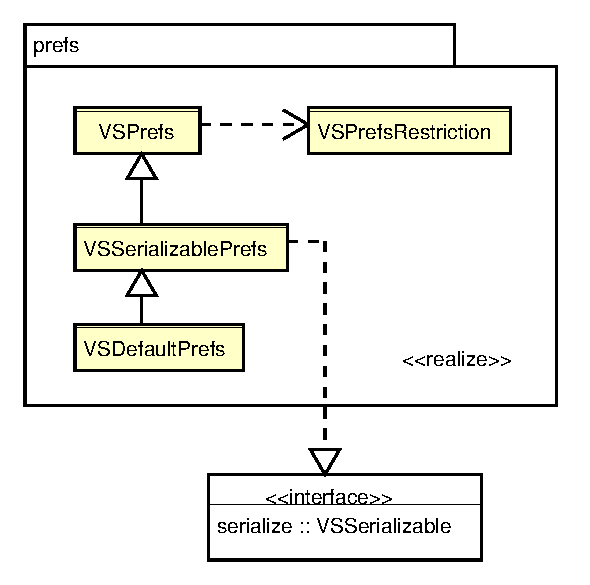
\includegraphics[width=7cm]{images/prefs}
	\caption{Das Paket \textit{prefs}}
	\label{fig:PackagePrefs}
\end{figure}

Jede Variable besteht aus einen Datentypen, einen Variablennamen und einer optionalen Beschreibung sowie einen Wert. Einige Datentypen unterst�tzen auch die Angabe von Minimal- und Maximalwerten (zum Beispiel besteht eine Prozentangabe aus einen Integerwert zwischen \textit{0} und \textit{100}), was mithilfe der \textit{VSPrefsRestriction}-Klasse implementiert wird. Da man beispielsweise bei Prozent ein \textit{\%} und bei Millisekunden ein \textit{ms} hinter der Variable sehen m�chte, kann f�r jede Variable auch ein optionaler Einheiten-String abgespeichert werden. 

Eine Variablenbeschreibung wird f�r die Darstellung im GUI verwendet, w�hrend der Variablenname eher f�r die interne Verwendung vom Simulator verwendet wird. Zum Beispiel hat die Variable \textit{message.prob.outage} (Verlustwahrscheinlichkeit einer Nachricht) die Variablenbeschreibung ``Nachrichtenverlustw'keit''. Wenn f�r eine Variable keine Beschreibung existiert so wird, wie auf Abbildung \ref{fig:SimulationseinstellungenExperten} anhand der Farbvariablen schon gesehen wurde, f�r die Anzeige einer Variable der Datentyp und der Variablenname verwendet. Variablennamen verwenden die auf Tabelle \ref{tb:VariablenPrefixe} angegebenen Prefixkonventionen. Alle verf�gbaren Typen wurden bereits in Tabelle \ref{tb:VariablenDatentypen} aufgelistet. \textit{VSPrefs} stellt f�r alle Variablentypen entsprechende Zugriffsmethoden zur Verf�gung.  

Im Folgenden werden nicht alle existierenden Methoden aufgelistet, da diese auch in der Quelltext-Dokumentation eingesehen werden k�nnen. Die Methoden werden nun nur anhand des Integer-Datentyps verdeutlicht. F�r alle anderen Typen gilt fast alles analog. F�r Integer stehen in \textit{VSPrefs} folgende Methoden zur Verf�gung:

\begin{itemize}
	\setlength{\itemsep}{-2mm}
	\item \textit{void setInteger(String key, Integer val)}
	\item \textit{void setInteger(String key, Integer val, String descr)}
	\item \textit{void setInteger(String key, int val)}
	\item \textit{void setInteger(String key, int val, String descr)}
	\item \textit{Integer getIntegerObj(String key)}
	\item \textit{int getInteger(String key)}
	\item \textit{java.util.Set<String> getIntegerKeySet()}
	\item \textit{void initInteger(String key, int val) }
	\item \textit{void initInteger(String key, int val, String descr) }
	\item \textit{void initInteger(String key, int val, String descr, int minValue, int maxValue) }
	\item \textit{void initInteger(String key, int val, String descr, int minValue, int maxValue, String unit) }
	\item \textit{void initInteger(String key, int val, String descr, VSPrefsRestriction.VSIntegerPrefsRestriction r) }
	\item \textit{void initInteger(String key, int val, String descr, VSPrefsRestriction.VSIntegerPrefsRestriction r, String unit) }
\end{itemize}

\begin{table}
	\fbox{
	\begin{tabular}{c|l|l}
		\textbf{Variablen-Prefix} & \textbf{Beschreibung}  & \textbf{Beispiel}\\
		\hline 
		\textit{col} & Farbvariablen & \textit{Color: col.background = Color-Objekt}\\
		\textit{div} & Diverse versteckte Variablen & \textit{Integer: div.window.loggsize = 300} \\
		\textit{keyevent} & Variablen, die Tastaturk�rzel definieren & \textit{Integer: keyevent.close = KeyEvent.VK\_C} \\
		\textit{lang} & Variablen, die Text beinhalten & \textit{String: lang.activate = aktivieren}\\
		\textit{message} & Variablen, die Nachrichten betreffen & \textit{Integer: message.prob.outage = 0}\\
		\textit{process} & Variablen, die Prozesse betreffen & \textit{Integer: process.prob.crash = 0}\\
		\textit{sim} & Allgemeine Simulationsvariablen & \textit{Integer: sim.process.num = 3}\\
	\end{tabular}
	}
	\caption{Konventionen f�r Variablennamen-Pr�fixe in \textit{VSDefautPrefs}}
	\label{tb:VariablenPrefixe}
\end{table}

Hierbei stellt \textit{key} den Variablennamen- und \textit{val} den Variablenwert dar. \textit{descr} ist eine optionale Variablenbeschreibung. Es k�nnen sowohl Java's Integer-Objekte, als auch Java's primitiver Integer-Typ \textit{int} verwendet werden. Ein \textit{int}-Wert wird intern allerdings als Integer-Objekt abgespeichert (f�r eine sp�tere Serialisierung, mehr dazu aber sp�ter) und macht somit keinen gro�en Unterschied. Die Methode \textit{getIntegerKeySet} gibt alle vorhandenen Integer-Variablennamen (\textit{key}s) als \textit{Set} zur�ck.

\textit{VSPrefs} bietet auch eine Reihe von \textit{initInteger}-Methoden an, welche sich von den \textit{setInteger}-Methoden dadurch unterscheiden, dass sie eine Variable nur einen Wert zuweisen, wenn sie vorher noch nicht initialisiert wurde, was durch \textit{setInteger} oder \textit{initInteger} selbst geschehen sein kann. Eine komplette �bersicht aller Methoden (auch f�r andere Datentypen) gibt es in der Quelltext-Dokumentation.

\textit{VSPrefs} speichert alle Integervariablen in einem \textit{HashMap<String,Integer>}-Objekt ab, wobei der String-Wert den Variablennamen \textit{key} angibt. F�r die Beschreibung \textit{descr}, den Einheiten-String \textit{unit} sowie m�glichen Minimal- und Maximalwerte werden separate Instanzen von \textit{HashMap} verwendet. Da alle \textit{HashMap}-Objekte synchronisiert sind, k�nnen alle Methoden von verschiednenen Threads gleichzeitig verwendet werden. 

\textit{VSSerializablePrefs} implementiert das Interface \textit{VSSerializable} und kann somit alle enthaltenen Daten in eine Datei abspeichern beziehungsweise laden. Auf die Serialisierung und Deserialisierung von Simulationen wird sp�ter genauer eingegangen.

Die Klasse \textit{VSDefaultPrefs} erweitert \textit{VSSerializablePrefs} und initialisiert bei Instantiierung automatisch alle verf�gbaren Simulationsvariablen mit ihren Standardwerten. Dort sind auch alle Spracheinstellungen abgelegt. Sollte jemand den Simulator in eine andere Sprache, zum Beispiel ins Englische, �bersetzen wollen, so mu� er lediglich diese Datei und die Protokoll-Klassen (mehr dazu sp�ter) editieren. Die Spracheinstellungen sind n�mlich in einem \textit{VSPrefs}--Objekt als versteckte String-Variablen abgespeichert. Spracheinstellungen f�r Protokolle wurden in den Protokollklassen direkt angegeben, da dies mehr Komfort f�r den Protokollentwickler bietet und f�r jede neue Textausgabe nicht st�ndig \textit{VSDefaultPrefs.java} editiert werden muss. 

Alle Variablen die als Prefix \textit{lang}, \textit{keyevent}, \textit{div} oder \textit{col} im Namen tragen, sind versteckte Variablen und werden in einem Editor nicht angezeigt. Im Expertenmodus sind hingegen nur Variablen die mit \textit{lang} und \textit{keyevent} beginnen versteckt. Somit lassen sich im Expertenmodus weitere Variablen vom Anwender editieren.

\subsection{Editorobjekte}

Wie Variablen intern abgespeichert werden ist bereits bekannt. F�r das Editieren der Variablen werden Editor-Objekte verwendet. Auf Abbildung \ref{fig:PackagePrefsEditors} ist die Klassenstruktur des dazugeh�rigen Paketes \textit{prefs.editors} angegeben. 

Die Basis eines Editors stellt die abstrakte Klasse \textit{VSAbstractEditor} dar, dem ein \textit{VSPrefs} Objekt zum Editieren �bergeben wird. Ein Editor stellt alle verf�gbaren nicht-versteckten Variablen des \textit{VSPrefs}-Objektes im GUI dar und bietet gleichzeitig die M�glichkeit alle Variablen dar�ber zu editieren an. F�r das Editieren von Farbwerten wird auf \textit{VSColorChooser} zur�ckgegriffen. Die Klasse \textit{VSEditorTable} ist f�r das \textit{JTable}-Objekt aus Java's Swing-Bibliothek zust�ndig, welches bei der graphischen Darstellung aller Variablen eingesetzt wird. Die abstrakte Klasse \textit{VSAbstractBetterEditor} wurde, wegen der �bersicht, als Zwischenschritt eingef�gt. 

\begin{figure}[h]
	\centering
	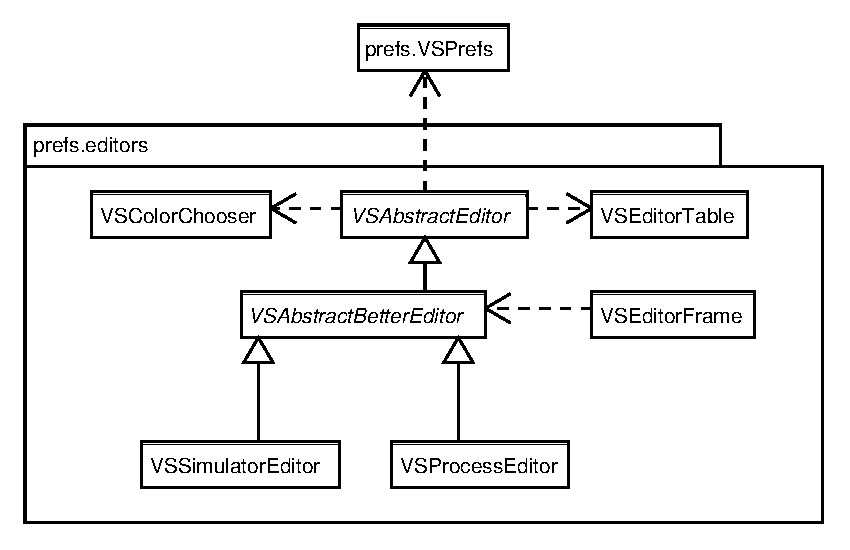
\includegraphics[width=10.5cm]{images/prefs-editors}
	\caption{Das Paket \textit{prefs.editors}}
	\label{fig:PackagePrefsEditors}
\end{figure}

Die Klasse \textit{VSSimulatorEditor} dient f�r das Editieren der globalen Simulationseinstellungen und \textit{VSProcessEditor} f�r das Editieren der Prozesseinstellungen sowie der dazugeh�rigen Protokollvariablen. Da diese beiden Klassen von \textit{VSAbstractBetterEditor} erben, k�nnen sie mithilfe von \textit{VSEditorFrame} in einem separaten Fenster angezeigt werden. Alternativ k�nnen die Editoren auch in der Sidebar im Tab ``Variablen'' angezeigt werden. Auf Abbildung \ref{fig:Simulationseinstellungen} wurde bereits ein \textit{VSEditorFrame} in Aktion gesehen. Auf Abbildung \ref{fig:NeueSimulationVariablen} wurde hingegen ein Prozesseditor in der Sidebar ge�ffnet. F�r Protokolle gibt es keine separate Editor-Klasse, da sie bereits vom Prozesseditor aus editiert werden k�nnen. Dabei iteriert der Prozesseditor �ber alle f�r den jeweiligen Prozess verf�gbaren Protokollobjekte und f�gt deren Variablen zus�tzlich in den Prozesseditor ein. Somit erscheinen die Prozess- und die dazugeh�rigen Protokollvariablen im selben Editor und bieten dem Benutzer so eine bessere �bersicht.

\section{Ereignisse}

\subsection{Funktionsweise von Ereignissen}

F�r jedes Ereignis existiert eine dazugeh�rige Klasse, welche die auszuf�hrenden Aktionen implementiert. Eine Instanz davon wird f�r eine sp�tere Ausf�hrung dem Task-Manager �bergeben. Auf den Task-Manager wird sp�ter noch genauer eingegangen. 
\begin{figure}[h]
	\centering
	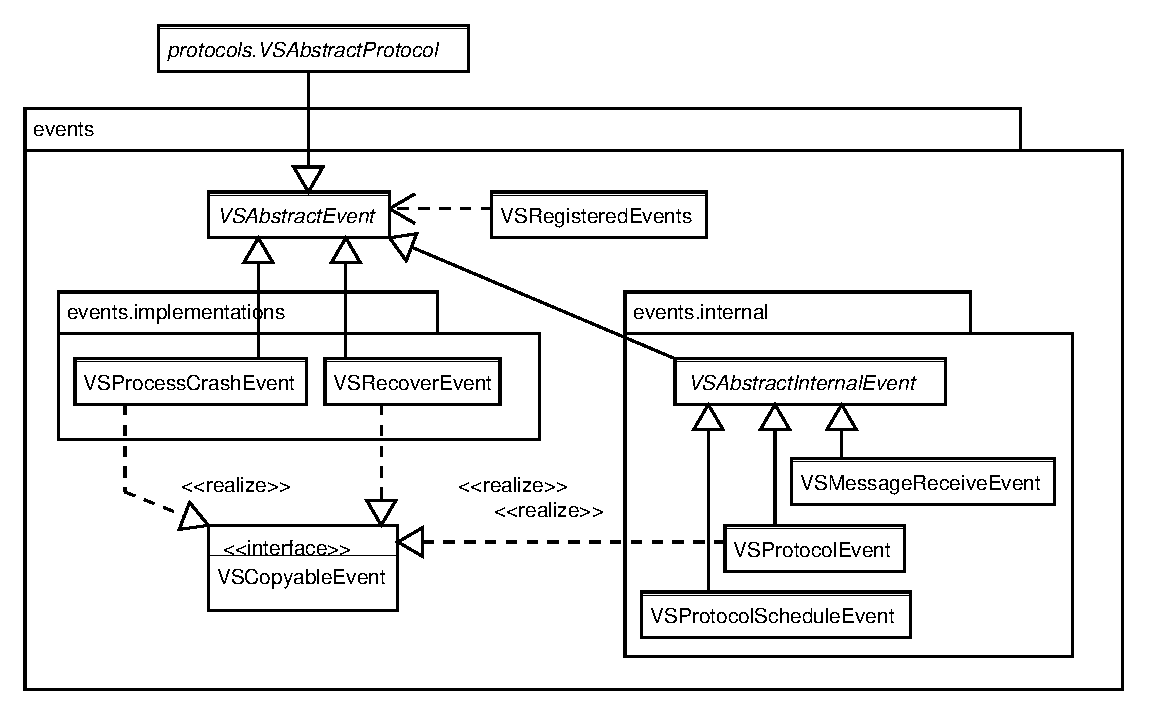
\includegraphics[width=13.5cm]{images/events}
	\caption{Die Pakete \textit{events} und \textit{events.*}}
	\label{fig:PackageEvents}
\end{figure}

Jedes programmierbare Ereignis mu�, bevor es vom Simulator verwendet werden kann, in der statischen Klasse \textit{VSRegisteredEvents} registriert werden. Da sich die Anzahl der verf�gbaren Ereignisklassen des Simulators bei Laufzeit nicht �ndert, gibt es keine Instanzen von \textit{VSRegisteredEvents}. Alle Methoden und Klassenattribute sind hier statisch. Wenn beispielsweise eigene Ereignisse implementiert werden, dann m�ssen alle neuen Ereignisse per Hand in die Datei \textit{VSRegisteredEvents.java} �bernommen- und der Simulator neu kompiliert werden.

In der Implementierung wird zwischen drei Haupttypen von Ereignissen unterschieden, die jeweils in verschiedenen Paketen liegen (Abbildung \ref{fig:PackageEvents}):

\begin{enumerate}
	\item \textit{events.implementations}: In diesem Paket befinden sich alle Ereignisse, die ohne weitere Spezialbehandlung vom Simulator eingesetzt werden k�nnen und vom Benutzer direkt im Ereigniseditor programmierbar sind. 
		\begin{itemize}
			\item \textit{VSProcessCrashEvent}: Dieses Ereignis l�sst den dazugeh�rigen Prozess abst�rzen.
			\item \textit{VSProcessRecoverEvent}: Dieses Ereignis l�sst den dazugeh�rigen Prozess wiederbeleben.
		\end{itemize}

	\item \textit{events.internal}: In diesem Paket befinden sich alle Ereignisse, die vom Simulator intern verwendet werden. Bevor der Simulator von diesen Ereignissen Gebrauch machen kann, muss er vorher einige Spezialbehandlungen durchf�hren.
		\begin{itemize}
			\item \textit{VSAbstractInternalEvent}: Diese Klasse stellt weitere Methoden zur Verf�gung, die von allen internen Ereignissen ben�tigt werden. Derzeit betrifft dies nur Methoden zur Serialisierung der gegebenen Objekte. Auf die Serialisierung (Abspeichern/Laden) von Simulationen wird sp�ter noch genauer eingegangen.
			\item \textit{VSMessageReceiveEvent}: Diese Klasse wird f�r die Ankunft einer Nachricht bei einem Empf�ngerprozess ben�tigt. Sie kapselt die eigentliche Nachricht und �berpr�ft, ob der Empf�ngerprozess das zur Nachricht dazugeh�rige Protokoll versteht. Diese Klasse �berpr�ft auch die Simulationseinstellung ``Nur relevante Nachrichten anzeigen'' und entscheidet, ob die Nachricht nach Eintreffen in der Visualisierung und im Loggfenster ber�cksichtigt werden soll oder nicht.
			\item \textit{VSProtocolEvent}: Diese Klasse implementiert gleichzeitig vier verschiedene Ereignisse: Das Aktivieren/Deaktivieren eines Servers/Clients eines gegebenen Protokolls. Der Ereigniseditor berechnet anhand der verf�gbaren Protokolle automatisch alle m�glichen Kombinationen und bietet sie dem Anwender in seiner Auswahl an. F�r alle dieser vier Ereignisse wird jeweils ein Objekt von \textit{VSProtocolEvent} verwendet, jedoch mit jeweils anderen Attributwerten.  
			\item \textit{VSProtocolScheduleEvent}: Diese Klasse wird f�r die Wecker-Ereignisse ben�tigt. Wecker-Ereignisse k�nnen nur von Protokollen (mehr dazu sp�ter) erstellt werden. \textit{VSProtocolScheduleEvent} besitzt eine Referenz auf das gegebene Protokoll und ruft bei Ereigniseintrittszeit entweder die Methode \textit{onServerScheduleStart} bei einem Server- oder \textit{onClientScheduleStart} bei einem Clientprotokoll auf. 
		\end{itemize}
	\item \textit{protocols.implementations}: In diesem Paket befinden sich alle Protokollimplementierung. Jedes Protokoll besitzt hier seine eigene Klasse. Alle Protokolle erben hierbei von der auf Abbildung \ref{fig:PackageEvents} zu sehenden Klasse \textit{protocols.VSAbstractProtocol}. Da \textit{protocols.VSAbstractProtocol} von \textit{events.VSAbstractEvent} erbt, kann ein Protokollobjekt auch als Ereignis eingesetzt werden. Ein solches Ereignis ruft bei Eintritt entweder die Methode \textit{onServerStart} oder die Methode \textit{onClientStart} des Protokolls auf, was einer Server- beziehungsweise einer Clientanfrage entspricht. Die Implementierung von Protokollen wird sp�ter genauer behandelt. 
\end{enumerate}

Alle Ereignisse, die das Interface \textit{VSCopyableEvent} implementieren, k�nnen vom Anwender im Ereigniseditor mit einem Rechtsklick kopiert werden und m�ssen die Methode \textit{initCopy(VSAbstractEvent copy)} implementieren. Dort werden dann alle relevanten Attribute in das neue Ereignis \textit{copy} kopiert. 

Alle Ereignisklassen erweitern die abstrakte Klasse \textit{VSAbstractEvent} und m�ssen folgende abstrakten Methoden implementieren:

\begin{itemize}
	\item \textit{abstract public void onInit()}: Bevor ein Ereignisobjekt vom Simulator verwendet werden kann, mu� es initialisiert werden. Je nach Ereignis k�nnen hier verschiedene Werte initialisiert werden. Diese Methode wird pro Ereignisobjekt nach Erstellung nur ein einziges Mal ausgef�hrt. 
	\item \textit{abstract public void onStart()}: Diese Methode wird jedes Mal ausgef�hrt, wenn das Ereignis eintritt. Sie stellt somit das Kernst�ck eines Ereignisses dar. 
\end{itemize}

Des Weiteren werden folgende nicht-abstrakte Methoden von \textit{VSAbstractEvent} vererbt:

\begin{itemize}
	\item \textit{public void logg(String message)}: Diese Methode schreibt eine Loggnachricht in das Simulationsloggfenster.
	\item \textit{public VSAbstractEvent getCopy()}: Diese Methode erstellt vom aktuellen Ereignis eine Kopie, worauf eine Referenz zur�ckgegeben wird. Alle Ereignisse die kopiert werden k�nnen m�ssen ebenso das Interface \textit{VSCopyableEvent} implementieren. Wenn ein Ereignis dies nicht tut und \textit{getCopy()} aufgerufen wird, dann wird von Java die Ausnahme \textit{exceptions.VSEventNotCopyable} geworfen.
	\item \textit{public VSAbstractEvent getCopy(VSInternalProcess process)}: Diese Methode erstellt vom aktuellen Ereignis ebenfalls eine Kopie, jedoch mit dem Unterschied, dass das Ereignis einem anderen Prozess zugewiesen wird. 
\end{itemize}

Jede Ereignisklasse hat au�erdem Zugriff auf folgende Attribute, die von \textit{VSAbstractEvent} vererbt werden:

\begin{itemize}
	\item \textit{protected VSPrefs prefs}: Eine Referenz auf das Simulationseinstellungsobjekt. Hier�ber lassen sich alle Simulationseinstellungen beziehen. 
	\item \textit{protected VSAbstractProcess process}: Eine Referenz auf das Prozessobjekt des jeweiligen Prozesses, auf welches das Ereignis angewendet wird.
\end{itemize}

Da \textit{VSAbstractEvent} die Klasse \textit{VSSerializablePrefs} erweitert, k�nnen alle Ereignisse mit allen ihren Variablen serialisiert werden. Hierauf wird sp�ter nochmal eingegangen.

\subsection{Beispielimplementierung eines Ereignisses}

Im Folgenden wird als Beispiel die Implementierung des Prozessabsturzereignisses \textit{VSProcessCrashEvent} behandelt. Da die dazugeh�rige Klasse keine Attribute besitzt, verbleibt hier auch die \textit{initCopy}-Methode mit leerem Rumpf. Jede Ereignisklasse muss in \textit{onInit()} mit \textit{setClassname} den eigenen Klassennamen mitteilen. In \textit{onStart()} wird das eigentliche Ereignis ausgef�hrt. Hier wird obligatorisch �berpr�ft, ob der Prozess bereits abgest�rzt (hier eigentlich nicht Notwendig, verbessert aber die Lesbarkeit der Logik) ist und gegebenenfalls wird der Prozess dann zum Absturz bewegt. 

Der Task-Manager �berpr�ft bereits, ob der Prozess abgest�rzt ist oder nicht, d.h. ein Ereignis wird bei einem abgest�rztem Prozess gar nicht erst ausgef�hrt. Die einzige Ausnahme bildet ein Wiederbelebungsereignis (\text{VSProcessRecover}), welches vom Task-Manager ausgef�hrt wird, auch wenn der Prozess abgest�rzt ist. Mit \textit{logg} wird eine Nachricht (die �ber \textit{prefs} bezogen wird) in das Loggfenster geschrieben.
\begin{code}
package events.implementations;

import events.*;

public class VSProcessCrashEvent 
extends VSAbstractEvent implements VSCopyableEvent {
    public void initCopy(VSAbstractEvent copy) {
    }

    public void onInit() {
        super.setClassname(super.getClass().toString());
    }

    public void onStart() {
        if (!process.isCrashed()) {
            process.isCrashed(true);
            super.logg(prefs.getString("lang.crashed"));
        }
    }
}
\end{code}

In der Datei \textit{events/VSRegisteredEvents.java} muss in der \textit{init}-Methode f�r jedes programmierbare Ereignis ein Eintrag existieren. Die \textit{init}-Methode wird einmal beim Starten des Simulators ausgef�hrt:

\begin{code}
public static void init(VSPrefs prefs_) {
    .
    .
    .
    registerEvent("events.implementations.VSProcessCrashEvent",
                  "Prozessabsturz");
    .
    .
    .
}
\end{code}

Als Resultat kann das Prozessabsturzereignis nach Belieben via GUI programmieren- und eingesetzt werden.

\section{Zeitformate, Prozesse, Nachrichten sowie Task-Manager}

\subsection{Funktionsweise}

Das Paket \textit{core.time} auf Abbildung \ref{fig:PackageCoreTime} stellt lediglich die Klassen f�r die Vektor- und Lamportzeitstempel zur Verf�gung. F�r die normale lokale Prozesszeit wird aus Performancegr�nden keine eigene Klasse, sondern ein einfaches \textit{long}-Attribut des Prozessobjektes verwendet.

\begin{figure}[h]
	\centering
	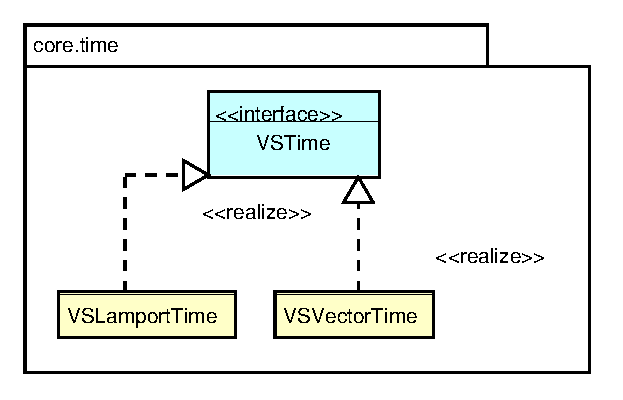
\includegraphics[width=7cm]{images/core-time}
	\caption{Das Paket \textit{core.time}}
	\label{fig:PackageCoreTime}
\end{figure}

Auf Abbildung \ref{fig:PackageCore} ist stark vereinfacht das Paket \textit{core} dargestellt. F�r jedes auszuf�hrendes Ereignis wird eine Instanz von \textit{VSTask} ben�tigt, welche die Ereigniseintrittszeit als Attribut abgespeichert hat sowie eine Referenz auf das Objekt des auszuf�hrenden Ereignisses (\textit{VSAbstractEvent}) und dem Prozessobjekt besitzt. Geplante \textit{VSTask}-Instanzen werden f�r eine sp�tere Ausf�hrung dem Task-Manager �bergeben.

Die Kapselung eines \textit{VSAbstractEvent}-Objektes in einem \textit{VSTask}-Objekt erlaubt es, dass die selbe \textit{VSAbstractEvent}-Instanz mehrmals auf einmal im Task-Manager geplant werden kann. Ohne dieser Kapselung g�be es f�r jedes Ereignis lediglich nur eine einzige m�gliche Eintrittszeit. Von dieser M�glichkeit wird zum Beispiel bei den Server- und Clientanfragen eines Protokollobjektes Gebrauch gemacht. F�r jedes Protokoll kann der Anwender in einer Simulation beliebig viele Anfragen programmieren, wobei f�r jede Anfrage stets das selbe Protokollobjekt als Ereignis verwendet wird.

\begin{figure}[h]
	\centering
	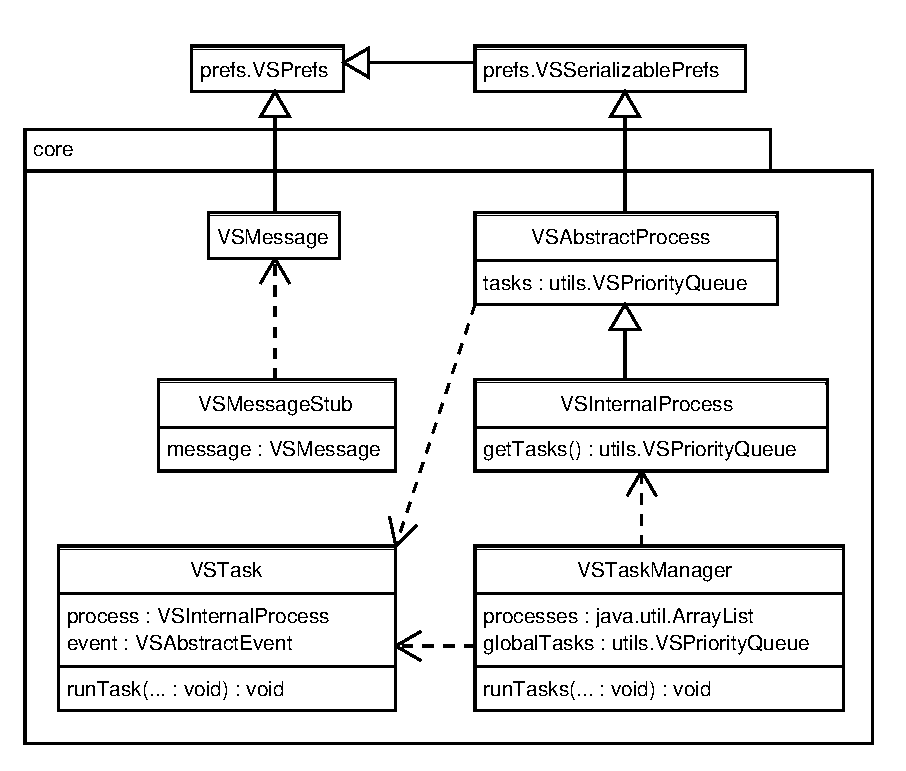
\includegraphics[width=10.0cm]{images/core}
	\caption{Das Paket \textit{core}}
	\label{fig:PackageCore}
\end{figure}

Jede Simulation besitzt genau eine Instanz von \textit{VSTaskManager}. Eine Instanz dieser Klasse stellt den Task-Manager dar. Er verwaltet alle \textit{VSTask}-Instanzen und �berpr�ft periodisch, ob es auszuf�hrende Ereignisse gibt. Der Task-Manager unterscheidet zwischen globalen und lokalen Ereignissen. Hierbei werden alle globalen Ereignisse (gekapselt in einem \textit{VSTask}-Objekt) in einer Priorit�ts-Warteschlange abgelegt. Die Priorit�ts-Warteschlange stellt hierbei die korrekte Ereigniseintrittsreihenfolge sicher. Da sich die lokalen Zeiten aller beteiligten Prozesse voneinander unterscheiden k�nnen, muss f�r jeden Prozess eine separate lokale Priorit�ts-Warteschlange verwendet werden, auf die jedes Prozessobjekt seine eigene Referenz hat. In den lokalen Warteschlangen sind die geplanten lokalen Ereignisse (auch gekapselt in einem \textit{VSTask}-Objekt) abgelegt. Der Task-Manager greift �ber eine \textit{java.util.ArrayList} auf alle Prozessobjekte zu und kann somit auch auf alle lokalen Warteschlangen zugreifen und verwalten.

Eine Instanz von \textit{VSMessage} stellt eine Nachricht dar, die von einem Prozess verschickt wird. F�r jedes Versenden einer Nachricht wird hiervon eine Instanz gebildet, wo der Senderprozess die zu verschickende Daten ablegt. Da \textit{VSMessage} von \textit{VSPrefs} erbt, k�nnen zwischen zwei Prozessen beliebige Datentypen (Tabelle \ref{tb:VariablenDatentypen}) �ber eine Nachricht verschickt werden. Anschlie�end wird f�r jeden Empf�ngerprozess das neues Ereignisobjekt der Klasse \textit{VSMessageReceiveEvent} angelegt, welches eine Referenz der verschickten Nachricht besitzt (Abbildung \ref{fig:Wrapping}). Danach wird ein \textit{VSTask}-Objekt instantiiert, wo die Referenz auf das Ereignisobjekt und das dazugeh�rige Prozessobjekt sowie die Ereigniseintrittszeit als Attribute gespeichert werden. Das \textit{VSTask}-Objekt wird dann dem Task-Manager �bergeben, der das dazugeh�rige Ereignis ausf�hrt, wenn die Ereigniseintrittszeit eingetroffen ist. Via Java-Polymorphie wird das \textit{VSMessageReceiveEvent}-Objekt in ein \textit{VSAbstractEvent} umgewandelt. 

Erw�hnenswert ist auch die Klasse \textit{VSMessageStub}, welche ein \textit{VSMessage} kapselt. Ihr Zweck ist das Verstecken einiger Methoden vor dem Protokoll-API, welches f�r die Erstellung eigener Protokolle dient. Der Protokoll-Entwickler soll m�glichst nichts falsch machen k�nnen und deswegen soll den Protokoll-API ein eingeschr�nkter Funktionsumfang zur Verf�gung gestellt werden. Da sich \textit{VSMessageStub} im selben Paket wie \textit{VSMessage} befindet, kann \textit{VSMessageStub} auf paket-private Methoden von \textit{VSMessage} zugreifen. Protokolle hingegen werden in einem anderen Paket implementiert und haben somit keinen Zugriff auf diese paket-privaten Methoden. Zwar kann der Protokollentwickler ein eigenes \textit{VSMessageStub}-Objekt anlegen, jedoch kann er auf diese Weise besser unterscheiden auf welche Methoden er zugreifen sollte und auf welche nicht. Das Protokoll-API wird sp�ter genauer behandelt. 

\begin{figure}[h]
	\centering
	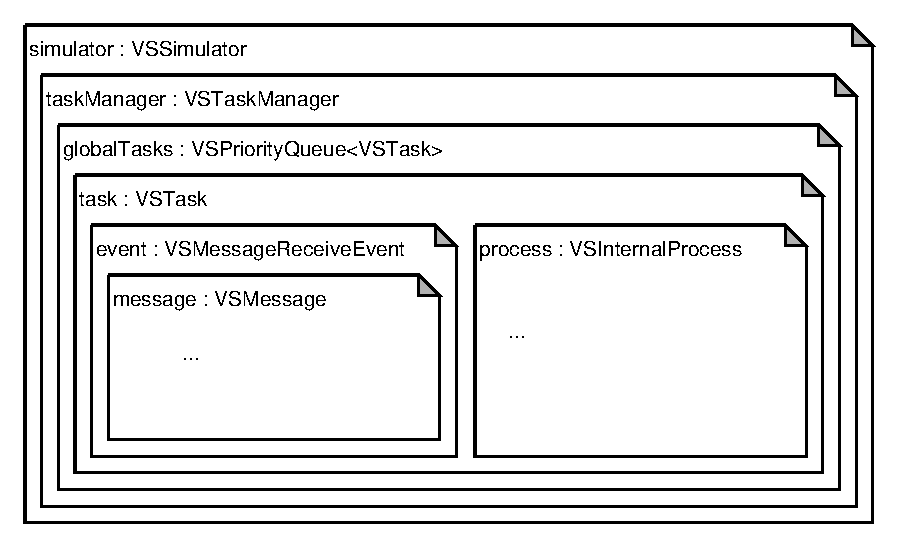
\includegraphics[width=11.0cm]{images/wrapping}
	\caption{Gekapseltes \textit{VSMessage} im \textit{VSMessageReceiveEvent}-Objekt}
	\label{fig:Wrapping}
\end{figure}

Der Task-Manager speichert anschlie�end in der globalen Warteschlange die Nachrichtenempfangsereignisse. Die Nachricht kommt bei einem Empf�ngerprozess an, sobald das Ereignis f�r den Empfang eintritt. F�r die korrekte Implementierung der Lamport- und Vektor-Zeitstempel wird jeder Nachricht automatisch eine Referenz auf die Lamport- sowie auf die Vektorzeit des sendenden Prozesses als Attribut beigef�gt. F�r die �berpr�fung des Protokolls wird in jeder Nachricht auch der Klassenname des jeweiligen Protokolls abgespeichert.

Eine Instanz von \textit{VSInternalProcess} repr�sentiert einen simulierten Prozess. Ein \textit{VSInternalProcess} stellt alle vom Simulator intern verwendeten Methoden zur Verf�gung, w�hrend ein \textit{VSAbstractProcess} lediglich Methoden hat, die der Protokollentwickler f�r die Erstellung eigener Protokolle verwenden darf. Da \textit{VSAbstractProcess} abstrakt ist und hiervon keine Instanz gebildet werden darf, muss f�r einen neuen Prozesses stets ein \textit{VSInternalProcess}-Objekt erstellt werden. Via Polymorphie wird dieses Objekt nach \textit{VSAbstractProcess} umgewandelt und so dem Protokoll-API zur Verf�gung gestellt. Beispielsweise darf mit \textit{getTasks()} nur vom Simulator intern auf die Priorit�ts-Warteschlangen zugegriffen werden, w�hrend man im Protokoll-API selbiges vermeiden sollte und auch gar nicht direkt m�glich ist. Hierf�r h�tte man auch ein Stub-Objekt \textit{VSProcessStub} implementieren k�nnen. Da aber so gut wie alle paar Millisekunden auf die Methoden von \textit{VSInternalProcess} zugegriffen wird, wurde hier aus Performancegr�nden der Weg �ber eine Vererbungungsstufe preferiert. 

Alle einstellbaren Prozessvariablen werden von der Klasse \textit{VSPrefs} vererbt. Damit bei Neuberechnungen die Variablen nicht dauernd �ber eine \textit{HashMap} von \textit{VSPrefs} zugegriffen werden mu�, speichert \textit{VSInternalProcess} aus Performancegr�nden einige Variablen als lokale Kopie ab. Zum Beispiel wird f�r die lokale Prozesszeit nicht auf das \textit{HashMap<String,Long>}-Objekt von \textit{VSPrefs}, sondern auf das Klassenattribut \textit{private long localTime} zugegriffen. Vor- und nach dem Editieren �ber den Prozesseditor werden die \textit{VSPrefs} beziehungsweise die lokalen Kopien auf den neusten Stand gebracht. Selbiges gilt f�r weitere Variablen wie zum Beispiel der Uhrabweichung eines Prozesses.

\subsection{Beispiel f�r die Erstellung von Prozessereignissen}

Anhand der Prozessabsturz- und Wiederbelebungsereignisse l��t sich wie folgt sehr gut demonstrieren, wie intern Ereignisse angelegt werden k�nnen:
\begin{code}
void createCrashAndRecoverExample(VSTaskManager taskManager,
                                  VSInternalProcess process) {
    VSAbstractEvent crashEvent = new VSProcessCrashEvent();
    VSTask localTask = new VSTask(process.getTime()+500, process, 
                                  crashEvent, VSTask.LOCAL);
    taksManager.addTask(localTask);

    VSAbstractEvent recoverEvent = new VSProcessRecoverEvent();
    VSTask globalTask = new VSTask(2000, process, 
                                   recoverEvent, VSTask.GLOBAL);
    taksManager.addTask(globalTask);
}
\end{code}

In diesem Beispiel wurden zwei Ereignisse (Absturz- und Wiederbelebung eines gegebenen Prozesses) angelegt. Das Absturzereignis tritt bei der aktuellen lokalen Prozesszeit plus \textit{500ms} ein, w�hrend das Wiederbelebungsereignis bei einer globalen Zeit von \textit{2000ms} stattfindet. F�r den Fall, dass das Wiederbelebungsereignis vor dem Absturzereignis eintritt wird es nicht ausgef�hrt, da der Prozess noch nicht abgest�rzt ist. 

\section{Protokolle}

\subsection{Funktionsweise des Protokoll-APIs}

\begin{figure}[h]
	\centering
	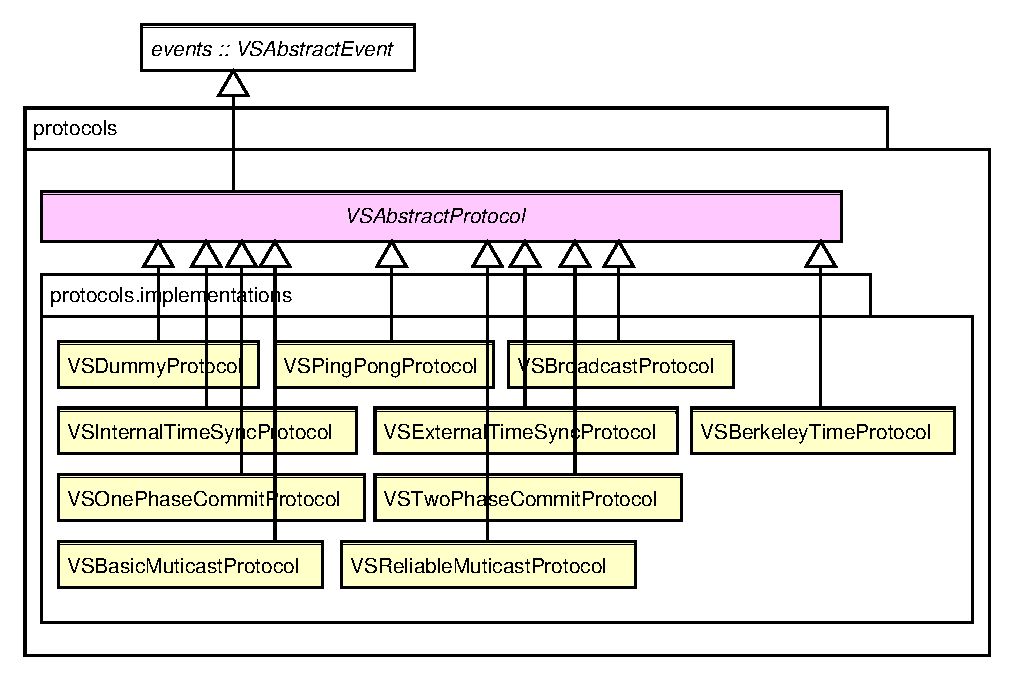
\includegraphics[width=12cm]{images/protocols}
	\caption{Die Pakete \textit{protocols} und \textit{protocols.*}}
	\label{fig:PackageProtocols}
\end{figure}

In diesem Abschnitt wird auf die Implementierung der Protokolle und das Protokoll-API eingegangen. Im Protokoll-API wird in der Regel nicht direkt auf den Task-Manager und auf die explizite Instantiierung von Ereignisobjekten zur�ckgegriffen. Das wird alles vom API automatisch gemacht.

Auf Abbildung \ref{fig:PackageProtocols} sind die Pakete \textit{protocols} und \textit{protocols.implementations} dargestellt, welche f�r die Protokollimplementierungen zust�ndig sind. \textit{VSAbstractProtocol} stellt lediglich gemeinsame Methoden und Attribute zur Verf�gung, die von allen Protokollen verwendet werden k�nnen. Jedes Protokoll hat im Paket \textit{protocols.implementations} seine eigene Klasse, die von \textit{VSAbstractProtocol} erbt. Im Prinzip besitzt jedes Prozessobjekt von jedem Protokoll seine eigene Instanz. Bei \textit{10} Protokollen und \textit{3} beteiligten Prozessen werden also \textit{30} Protokollobjekte verwendet. Jedes Protokollobjekt verwaltet sowohl die Server- als auch die Clientseite eines Protokolls auf einmal. Dabei merkt sich \textit{VSAbstractProtocol} anhand eines Flags ob der aktuelle Kontext server- oder clientbezogen ist und f�hrt dementsprechend beim Eintreffen von Ereignissen die Server- beziehungsweise Clientmethoden des Protokolls auf. \textit{VSAbstractProtocol} �berpr�ft auch, ob ein Client oder ein Server �berhaupt aktiviert ist. 

\begin{figure}[h]
	\centering
	\includegraphics[width=10cm]{images/ss-protokollvariablen}
	\caption{Protokollvariablen im Prozesseditor}
	\label{fig:Protokollvariablen}
\end{figure}

Es ist bereits bekannt, dass Protokolle im Prozesseditor editierbare Variablen haben k�nnen. Da \textit{VSAbstractProtocol} von \textit{VSAbstractEvent} erbt, was wiederum von \textit{VSPrefs} erbt, werden alle Protokollvariablen einfach in die Mutterklasse \textit{VSPrefs} abgelegt. Zum Beispiel kann mit \textit{super.setBoolean(``test'', true);} eine neue Protokollvariable \textit{test} mit dem Standardwert \textit{true} angelegt werden. Diese Variable erscheint dann automatisch im Prozesseditor. 

Da der Simulator daf�r ausgelegt wurde eigene Protokolle zu implementieren, werden im Folgenden alle verf�gbaren Protokoll-API-Methoden etwas ausf�hrlicher als gewohnt beschrieben. Jede Protokollklasse mu� die folgenden Methoden implementieren:

\begin{itemize}
	\setlength{\itemsep}{-2mm}
	\item Einen �ffentlichen (\textit{public}) Konstruktor. Der Konstruktor mu� angeben, ob bei dem gegebene Protokoll der Client oder der Server die Anfragen startet. 
	\item \textit{abstract public void onClientInit()}: Bevor das Protokollobjekt benutzt werden kann, mu� es initialisiert werden. Diese Methode wird vor dem ersten Verwenden des Protokolls innerhalb einer Simulation ausgef�hrt. In der Regel werden hier Protokollvariablen unter Verwendung von \textit{VSPrefs} und Attribute der Protokollklasse initialisiert. Die hier initialisierten Protokollvariablen lassen sich vom Benutzer im Prozesseditor des jeweiligen Prozesses editieren.
	\item \textit{abstract public void onClientReset()}: Diese Methode wird jedes Mal ausgef�hrt, wenn die Simulation zur�ckgesetzt wird.
	\item \textit{abstract public void onClientStart()}: Diese Methode wird nur ben�tigt, wenn der Client immer die Anfragen startet. Diese Methode generiert in der Regel immer eine Clientanfrage, die via \textit{VSMessage}-Objekt an alle anderen beteiligten Prozesse verschickt wird.
	\item \textit{abstract public void onClientRecv(VSMessage message)}: Diese Methode wird jedes Mal Ausgef�hrt, wenn eine Servernachricht \textit{message} bei dem Client eintrifft. 
	\item \textit{abstract public void onClientSchedule()}: Diese Methode wird jedes Mal ausgef�hrt, wenn ein Weckerereignis eintritt. 
	\item \textit{public String toString()}: Diese Methode ist nur optional. Hiermit lassen sich die Loggnachrichten eines Protokolls anpassen. Wenn diese Methode in einer Protokollimplementierung ausgelassen wird, so wird stets die \textit{toString}-Methode der Mutterklasse \textit{VSAbstractProtocol} verwendet.
\end{itemize}

F�r alle hier aufgelisteten Client-Methoden sind auch die korrespondierenden Server-Methoden anzugeben. Die Server-Methoden sind analog zu den Client-Methoden aufgebaut, wobei lediglich \textit{Client} durch \textit{Server} ausgetauscht werden mu�. 

Jede Protokollklasse bekommt folgende Methoden von \textit{VSAbstractProtocol} vererbt, welche allesamt vom Protokollentwickler verwendet werden k�nnen:

\begin{itemize}
	\setlength{\itemsep}{-2mm}
	\item \textit{pubic void sendMessage(VSMessage message)}: Hiermit verschickt das Protokoll eine Nachricht.
	\item \textit{pubic final boolean hasOnServerStart()}: Hiermit l��t sich bestimmen, ob der Server- oder der Client bei dem aktuellen Protokoll die Anfragen startet.
	\item \textit{pubic final boolean isServer()}: Hiermit l��t sich bestimmen, ob der aktuelle Prozess das aktuelle Protokoll serverseitig aktiviert hat. 
	\item \textit{pubic final boolean isClient()}: Hiermit l��t sich bestimmen, ob der aktuelle Prozess das aktuelle Protokoll clientseitig aktiviert hat. 
	\item \textit{pubic final void scheduleAt(long time)}: Diese Methode stellt einen Wecker, der zur angegebenen lokalen Prozesszeit eintritt. Nach Ablauf des Weckers wird, abh�ngig ob der aktuelle Kontext Client- oder Serverseitig ist, \textit{onClientSchedue} beziehungsweise \textit{onServerSchedule} ausgef�hrt. 
	\item \textit{pubic final void removeSchedules()}: Entfernt alle gesetzten Wecker des aktuellen Kontextes (Server oder Client).
	\item \textit{pubic final int getNumProcesses()}: Gibt die Anzahl an der Simulation beteiligten Prozesse zur�ck.
\end{itemize}

Bei der Implementierung von Protokollen k�nnen zus�tzlich auf die vererbten Attribute \textit{VSAbstractProcess process} und \textit{VSPrefs prefs} zugegriffen werden. Verf�gbare Methoden von \textit{VSPrefs} wurden bereits behandelt. �ber \textit{prefs} lassen sich alle globalen Simulationseinstellungen abrufen (zum Beispiel die Simulationsvariable die Angibt, ob Prozesse eigene Nachrichten empfangen: \textit{bool recvOwn = prefs.getBoolean(``sim.message.own.recv'')}). Folgende Prozessmethoden d�rfen auf \textit{process} aus dem Protokoll-API verwendet werden:

\begin{itemize}
	\setlength{\itemsep}{-2mm}
	\item \textit{public float getClockVariance()}: Gibt die Uhrabweichung zur�ck. 
	\item \textit{public void setClockVariance(float clockVariance)}: Setzt die Uhrabweichung des Prozesses.
	\item \textit{public long getGlobalTime()}: Gibt die aktuelle globale Simulationszeit zur�ck.
	\item \textit{public long getTime()}: Gibt die aktuelle lokale Prozesszeit zur�ck.
	\item \textit{public void setTime(long time)}: Setzt die aktuelle lokale Prozesszeit.
	\item \textit{public long getLamportTime()}: Gibt die aktuelle Lamportzeit des Prozesses zur�ck.
	\item \textit{public void setLamportTime(long lamportTime)}: Setzt die aktuelle Lamportzeit des Prozesses.
	\item \textit{public void increaseLamportTime()}: Inkrementiert die Lamportzeit um eins.
	\item \textit{public void updateLamportTime(long lamportTime)}: Erneuert die Lamportzeit. Siehe Kapitel 2.6.1 wie die Lamportzeiten erneuert werden.
	\item \textit{public VSVectorTime getVectorTime()}: Gibt die aktuelle Vektor-Zeit des Prozesses zur�ck.
	\item \textit{public VSTime[] getLamportTimeArray()}: Gibt die gesamte Lamportzeitstempelhistorie des Prozesses zur�ck. Kann jeweils nach VSLamportTime umgewandelt werden.
	\item \textit{public VSTime getVectorTimeArray()}: Gibt die gesamte Vektor-Zeitstempel-Historie des Prozesses zur�ck. Kann jeweils nach VSVectorTime umgewandelt werden.
	\item \textit{public void updateVectorTime(VSVectorTime vectorTimeUpdate)}: Erneuert die Vektorzeit. Siehe Kapitel 2.6.1 wie die Vektorzeiten erneuert werden.
	\item \textit{public void increaseVectorTime()}: Inkrementiert die Vektorzeit an lokalem Index um eins.
	\item \textit{public int getProcessID()}: Gibt die PID zur�ck.
	\item \textit{public void setProcessID(int processID)}: Setzt die PID.
	\item \textit{public int getProcessNum()}: Gibt die Prozessnummer zur�ck. Dieser Wert unterscheidet sich von der PID. Die Prozessnummer gibt an, um den wievielten Prozess, beginnend bei 0, es sich handelt. 
	\item \textit{public int getRandomPercentage()}: Gibt einen Zufallswert zwischen \textit{0} und \textit{100} zur�ck.
	\item \textit{public boolean hasCrashed()}: Gibt \textit{true} zur�ck, wenn der Prozess w�hrend der aktuellen Simulation schon mal abgest�rzt ist.
	\item \textit{public boolean isCrashed()}: Gibt \textit{true} zur�ck, wenn der Prozess aktuell abgest�rzt ist.
	\item \textit{public void isCrashed(boolean isCrashed)}: Hiermit kann man den Prozess abst�rzen (\textit{isCrashed = true}) und wiederbeleben (\textit{isCrashed = false}) lassen.
\end{itemize}

In der Regel werden in Protokollen auch Nachrichten (\textit{VSMessage}) verschickt. Folgende Methoden d�rfen davon im Protokoll-API verwendet werden:

\begin{itemize}
	\setlength{\itemsep}{-2mm}
	\item \textit{public VSMessage()}: Der Standardkonstruktor f�r die Erstellung einer neuen Nachricht.
	\item \textit{public int getmessageID()}: Gibt die Nachrichten-ID zur�ck.
	\item \textit{public boolean equals(VSMessage message)}: Hiermit l��t sich �berpr�fen, ob eine weitere Nachricht die selbe NID besitzt (wobei es sich dann um die selbe Nachricht handeln w�rde).
\end{itemize}

Folgende weitere Methoden von \textit{VSMessage} k�nnen bei Erhalt einer Nachricht verwendet werden:

\begin{itemize}
	\setlength{\itemsep}{-2mm}
	\item \textit{public String getName()}: Gibt den Namen des zur Nachricht dazugeh�rigen Protokolls zur�ck. Diese Methode funktioniert nur bei empfangenen Nachrichten richtig.
	\item \textit{public String getProtocolClassname()}: Gibt den Klassennamen des zur Nachricht dazugeh�rigen Protokolls zur�ck. Diese Methode funktioniert nur bei empfangenen Nachrichten richtig.
	\item \textit{public VSAbstractProcess getSendingProcess()}: Gibt eine Referenz auf den Senderprozess zur�ck. Diese Methode funktioniert nur bei empfangenen Nachrichten richtig.
	\item \textit{public long getLamportTime()}: Gibt die Lamportzeit des Senderprozesses zur�ck. Diese Methode funktioniert nur bei empfangenen Nachrichten richtig.
	\item \textit{public VSVectorTime getLamportTime()}: Gibt die Vektorzeit des Senderprozesses zur�ck. Diese Methode funktioniert nur bei empfangenen Nachrichten richtig.
	\item \textit{public boolean isServerMessage()}: Hiermit l��t sich entscheiden, ob es sich um eine Server- oder eine Clientnachricht handelt. Diese Methode funktioniert nur bei empfangenen Nachrichten richtig.
\end{itemize}

Wenn �ber eine Nachricht Daten verschickt werden sollen, so werden die von \textit{VSPrefs} vererben Methoden verwendet. 

\subsection{Beispielimplementierung eines Protokolls}

Im Folgenden wird die Implementierung des zuverl�ssigen Multicast-Protokolls \textit{VSReliableMulticastProtocol.java} als Beispiel aufgef�hrt. Die Funktionsweise des Protokolls wurde bereits in Kapitel 2.5.10 beschrieben. Client- und Serverseite werden in der selben Klasse implementiert.

Im Konstruktor mu� stets angegeben werden, ob beim gegebenen Protokoll der Client oder der Server die Anfragen startet. Mit \textit{HAS\_ON\_CLIENT\_START} wird dem API mitgeteilt, dass der Client die Anfragen startet. F�r \textit{HAS\_ON\_SERVER\_START} und Serveranfragen gilt Selbiges analog. Da ein Protokoll auch ein \textit{VSAbstractEvent} ist, muss auch hier im Konstruktor mit \textit{setClassname} der Klassenname des aktuellen Protokolls angegeben werden:
	
\begin{code}
package protocols.implementations;

import java.util.ArrayList;
import java.util.Vector;
import protocols.VSAbstractProtocol;
import core.VSMessage;

public class VSReliableMulticastProtocol 
	extends VSAbstractProtocol {
    public VSReliableMulticastProtocol() {
        super(VSAbstractProtocol.HAS_ON_CLIENT_START);
        super.setClassname(super.getClass().toString());
    }
\end{code}

\subsubsection{Clientseite des Protokolls}

Das private Klassenattribut \textit{pids} wird f�r die Zwischenspeicherung beteiligter PIDs ben�tigt. Hier sind alle PIDs abgelegt, von denen noch Best�tigungsnachrichten erwartet werden. Hier werden als Standard-PIDs \textit{1} und \textit{3} verwendet. Die Methoden \textit{initVector} und \textit{initLong} wurden von \textit{VSPrefs} vererbt und initialisieren die Protokollvariablen \textit{pids} und \textit{timeout}, welche vom Benutzer im Prozesseditor editiert werden k�nnen (siehe Abbildung \ref{fig:Protokollvariablen} unter ``Reliable Multicast Client'' ganz unten):
\begin{code}
    private ArrayList<Integer> pids;

    public void onClientInit() {
        Vector<Integer> vec = new Vector<Integer>();
        vec.add(1); vec.add(3);
        super.initVector("pids", vec,
                         "PIDs beteiligter Prozesse");
        super.initLong("timeout", 2500, 
                       "Zeit bis erneute Anfrage", "ms");
    }
\end{code}

Wenn die Simulation zur�ckgesetzt wird, dann wird auch \textit{pids} reinitialisiert:
\begin{code}
    public void onClientReset() {
       	pids.clear();
        pids.addAll(super.getVector("pids"));
    }
\end{code}

In \textit{onClientStart} wird gepr�ft, ob eine Clientanfrage gestartet werden soll. Wenn dies der Fall ist (wenn von mindestens einem beteiligten Prozess noch keine Best�tigung erhalten wurde), wird ein neues Nachrichtenobjekt erstellt, und mit dem Inhalt \textit{Boolean: isMulticast=true} verschickt (intern wird hier f�r jeden Empf�ngerprozess ein \textit{VSMessageReceiveEvent} erzeugt). Mit \textit{scheduleAt} wird ein Wecker festgelegt, zur welchen lokalen Prozesszeit die Methode \textit{onClientSchedule} aufgerufen werden soll (intern wird hier ein \textit{VSProtocolScheduleEvent} erzeugt): 
\begin{code}
    public void onClientStart() {
        if (pids.size() != 0) {
            long timeout = super.getLong("timeout") 
                         + process.getTime();
            super.scheduleAt(timeout);

            VSMessage message = new VSMessage();
            message.setBoolean("isMulticast", true);
            super.sendMessage(message);
        }
    }
\end{code}

Wenn eine Serverantwort eintrifft, dann wird \textit{onClientRecv} aufgerufen. Hier wird �berpr�ft, ob �berhaupt noch Multicast-Best�tigungen ben�tigt werden. Wenn dies der Fall ist, dann wird geschaut, ob es sich bei der Antwort um eine noch nicht eingetroffene Best�tigung handelt. Gegebenenfalls wird die jeweilige PID aus \textit{pids} entfernt. Wenn \textit{pids} leer ist, dann wurde von allen beteiligten Prozessen eine Best�tigung erhalten und der Client entfernt mit \textit{removeSchedules} alle seine derzeit programmierten Wecker.

\begin{code}
    public void onClientRecv(VSMessage recvMessage) {
        if (pids.size() != 0 && recvMessage.getBoolean("isAck")) {
            Integer pid = recvMessage.getIntegerObj("pid");

            if (pids.contains(pid)) 
                pids.remove(pid);
            else 
                return;

            super.logg("ACK von Prozess " + pid + " erhalten!");

            if (pids.size() == 0) {
                super.logg("ACKs von allen beteiligten " +
                           " Prozessen erhalten!");

                super.removeSchedules();
            }
        }
    }
\end{code}

F�r das erneute Verschicken einer Clientanfrage ruft \textit{onClientSchedule} lediglich die Methode \textit{onClientStart} auf, die wiederum einen neuen Wecker planen kann:
\begin{code}
    public void onClientSchedule() {
        onClientStart();
    }
\end{code}

\subsubsection{Serverseite des Protokolls}

Die Serverseite des Protokolls speichert im Attribut \textit{ackSent} ab, ob es bereits eine Best�tigung des Multicasts verschickt hat oder nicht. In diesem Protokoll werden in \textit{onServerInit} keine Initialisierungen vorgenommen. Demnach gibt es f�r den Benutzer auch keine serverseitigen Protokollvariablen zu editieren. Beim Zur�cksetzen der Simulation wird lediglich \textit{ackSent} auf den Ursprungswert \textit{false} gesetzt:
\begin{code}
    private boolean ackSent = false;

    public void onServerInit() { }

    public void onServerReset() {
        ackSent = false;
    }
\end{code}

Wenn der Server eine Clientanfrage erhalten hat, so �berpr�ft der Server, ob es sich um eine Multicast-Nachricht handelte. Anschlie�end wird gegebenenfalls die Best�tigungsnachricht mit \textit{Boolean: isAck=true} und der Server-PID verschickt. Je nachdem ob bereits eine Best�tigung verschickt wurde oder nicht wird eine andere Nachricht geloggt: 
\begin{code}
    public void onServerRecv(VSMessage recvMessage) {
        if (recvMessage.getBoolean("isMulticast")) {
            VSMessage message = new VSMessage();
            message.setBoolean("isAck", true);
            message.setInteger("pid", process.getProcessID());
            super.sendMessage(message);

            if (ackSent) {
                super.logg("ACK erneut versendet");
            } else {
                super.logg("ACK versendet");
                ackSent = true;
            }
        }
    }
\end{code}

Der Server benutzt in diesem Beispiel keinen Wecker. Dementsprechend hat die Methode \textit{onServerSchedule} auch einen leeren Rumpf:
\begin{code}
    public void onServerSchedule() { }
}
\end{code}

\subsection{Erstellung eigener Protokolle (Schnelldurchlauf)}

Hier werden alle Schritte zusammengefasst, die f�r die Erstellung eines eigenen Protokolls \textit{VSMyProtocol} durchgef�hrt werden m�ssen.

\begin{enumerate}
	\item VS-Simulator Quelltext beziehen und in das Verzeichnis \textit{vs/sources/protocols/implementations} wechseln.
	\item Das Template-Protokoll \textit{VSDummyProtocol.java} nach \textit{VSMyProtocol.java} kopieren.
	\item \textit{VSDummyProtocol.java} editieren und den Klassennamen dort anpassen (\textit{VSDummyProtocol} $\rightarrow$ \textit{VSMyProtocol}).
	\item In das oberste Verzeichnis \textit{vs/} wechseln.
	\item Die Datei \textit{sources/events/VSRegisteredEvents.java} editieren, und in der \textit{init}-Methode folgende Zeile hinzuf�gen:
	\begin{code}
registerEvent("protocols.implementations.VSMyProtocol", 
              "Langer Name des Protokolls", // Langer Name
              "Neues Protokoll"); // Kurzer Name
	\end{code}
	\item Mit dem Befehl \textit{ant compile} die �nderungen �bernehmen und mit \textit{ant test} testen, ob der Simulator das Protokoll �bernommen hat. Hierbei wird der Simulator direkt aus dem Quellverzeichnis gestartet. ``Neues Protokoll'' sollte nun im Ereigniseditor programmiert werden k�nnen.
	\item Mit dem Befehl \textit{ant dist} das Archiv \textit{dist/lib/VS-Sim-Latest.jar} erstellen und verwenden.
\end{enumerate}

\section{GUI sowie Simulationsvisualisierung}

\subsection{Funktionsweise}

Das Paket \textit{simulator} (vereinfacht auf Abbildung \ref{fig:PackageProtocols} dargestellt) implementiert die eigentliche graphische Benutzeroberfl�che des Simulators. Ausnahmen sind die Editorklassen in \textit{prefs.editors} sowie \textit{utils.VSFrame}. 

Beim Starten des Simulators wird auf die Main-Methode, welche sich in \textit{VSMain} befindet, aufgerufen. Sie instantiiert ein \textit{VSDefaultPrefs}-Objekt, wo alle Standardeinstellungen des Simulators abgelegt sind. Anschlie�end wird ein \textit{VSSimulatorFrame} erzeugt, welches ein Simulatorfenster (wie bereits schon auf Abbildung \ref{fig:NeuesFenster} zu sehen war) implementiert. Das Simulatorfenster erstellt f�r jede neue Simulation jeweils ein Objekt von \textit{VSSimulator}. Jede Simulation hat im Simulationsfenster einen eigenen Tab. Auf Abbildung \ref{fig:NeuErstellteSimulation} wurde bereits eine neue Simulation erstellt, wo auch unten links der dazugeh�rige Tab mit der Beschriftung ``Simulator 1'' zu sehen ist. Jede Simulation besitzt dabei eine eigene Simulationsnummer, die bei jeder neuen Simulation um eins inkrementiert wird. Jedes \textit{VSSimulator}-Objekt greift auf \textit{VSSimulatorVisualization} zur�ck, was die Simulationsvisualisierung (Abbildung \ref{fig:Visualisierung}) implementiert. 

\textit{VSSimulatorVisualization} greift auf Java's Grafikbibliothek Java2D zur�ck und ist aus Performancegr�nden mit dem Simulationsverlauf stark verzahnt \cite{Games}. Klassenattribute, dessen Wert sich nie �ndert, wurden stets als \textit{final} deklariert. Attribute, die von Konfigurationen oder Einstellungen abh�ngig sind, die sich nur nach Konfigurations�nderung oder Vergr��ern beziehungsweise Verkleinern des Simulationsfensters �ndern (Werte, die f�r die Berechnung des Sekunden-Gatters notwendig sind), werden nur wenn es n�tig ist neu berechnet. 

\begin{figure}[h]
	\centering
	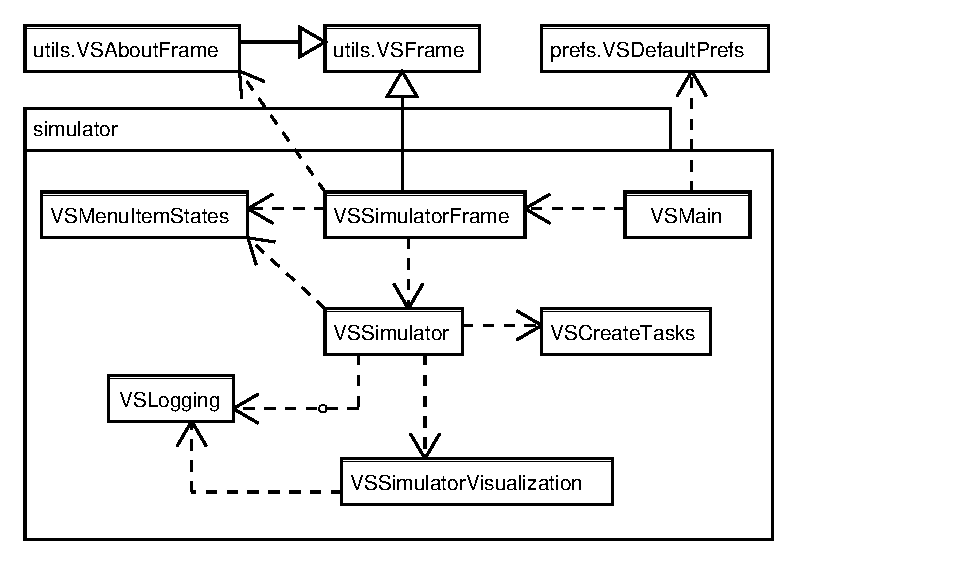
\includegraphics[width=11.0cm]{images/simulator}
	\caption{Das Paket \textit{simulator}}
	\label{fig:PackageProtocols}
\end{figure}

Die Klasse \textit{VSMenuItemStates} wird f�r die Synchronisierung des Simulationsstatusses, der Toolbar und des Simulations-Men�s (beide Letztere auf Abbildung \ref{fig:Toolbar} zu sehen) verwendet. Abh�ngig davon kann der Benutzer bestimmte Aktionen durchf�hren oder nicht (beispielsweise kann eine Simulation nur pausiert werden, wenn sie aktuell abgespielt wird). Alle hier m�glichen Aktionen wurden bereits in Kapitel 2.1 im Abschnitt ``Die Toolbar'' behandelt. 

Die Klasse \textit{VSCreateTask} wird vom Ereigniseditor verwendet. Der Ereigniseditor (Abbildung \ref{fig:SidebarMitEreignissen}) wird in der Klasse \textit{VSSimulator} implementiert. Hinter jeder Ereignisauswahl verbirgt sich intern ein \textit{VSCreateTask}-Objekt, welches definiert wie das jeweilige Ereignis anzulegen ist.

\textit{VSLogging} kapselt ein \textit{javax.swing.JTextArea}-Objekt, wo alle Nachrichten geloggt werden. Hier werden alle Loggfunktionen (inklusive Loggfilter sowie tempor�re Deaktivierung des Loggen) implementiert. Die \textit{JTextArea} wird dem \textit{VSSimulator}-Objekt �bergeben und dort dargestellt. F�r den Loggfilter wird intern auf das Java-Standardpaket \textit{java.util.regex} zugegriffen, womit anhand von regul�ren Ausdr�cken in Java-Syntax die Loggs gefiltert werden k�nnen.

\subsection{Threads und Zeitsynchronisierung}

Ziel vom Simulator ist es bis auf jede Millisekunde genau simulieren zu k�nnen. Jede simulierte Sekunde soll relativ zur echten Zeit fortschreiten. Die Simulationsabspielgeschwindigkeit l��t sich bei den Simulationseinstellungen unter ``Abspielgeschwindigkeit der Simulation'' (Float: \textit{sim.clock.speed}) einstellen. Damit dies gew�hrleistet wird, mu� folgendes ber�cksichtigt werden:

\begin{itemize}
	\item Das Zeichnen der Visualisierung ben�tigt pro Aktualisierung einige Millisekunden. Dies ist der rechen-intensivste Teil des Simulators. Hier werden st�ndig mathematische Berechnungen (wie zum Beispiel die Gerade einer Nachrichtenlinie, die automatische Skalierung des Diagramms die sich automatisch an die Fenstergr��e und der Simulationsdauer anpasst und vieles mehr).
	\item Das Neuberechnen der Simulation ben�tigt pro Aktualisierung einige Millisekunden. Hier wird insbesondere der Task-Manager beansprucht, der �berpr�ft, ob Ereignisse auszuf�hren sind und sie gegebenenfalls dann auch ausf�hrt.
	\item Jeder simulierte Prozess sollte mit selber Geschwindigkeit fortschreiten, und dies auf jedem Rechner wo der Simulator ausgef�hrt wird. Da Java-Threads nicht komplett plattformunabh�ngig sind (Threads sind im Betriebssystem implementiert), kann das Verhalten auf verschiedenen Rechnern minimal variieren. Au�erdem �bernimmt das Betriebssystem die Entscheidung, wann welcher Thread arbeiten darf. Au�er man synchronisiert Threads manuell so, dass sie den eigenen Anspr�chen entsprechen. Letzteres bedeutet aber auch mehr Programmieraufwand.
	\item Die Simulationszeit ist stets in Millisekunden angegeben, welche in einer \textit{long}-Variable abgespeichert wird. Somit kann eine Simulationszeit immer nur eine ganze Zahl sein. Berechnungsrundungsfehler wegen \textit{sim.clock.speed} m�ssen ber�cksichtigt werden.
	\item Der Simulator soll nicht st�ndig die komplette CPU des Anwender-Computers voll beanspruchen.
\end{itemize}

Es wurde folgende relativ einfache L�sung gew�hlt, bei der lediglich ein einziger Thread f�r die Visualisierung und die Berechnung der Simulation zust�ndig ist (alle Zeitangaben sind in Millisekunden). Der Algorithmus verl�uft leicht vereinfacht in folgender Form ab:

\begin{enumerate}
	\item Die simulierte globale Startzeit sei $s$ und die globale Zeit wo die Simulation aufh�rt sei $e$.
	\item Wenn $s > e$, dann $s := e$ setzen. 
	\item Neuberechnen und Zeichnen der Visualisierung zum Zeitpunkt $s$. Die dabei verstrichene Zeit sei $v$. 
	\item Wenn $s = e$, dann Simulation beenden.
	\item F�r einige Millisekunden den Thread pausieren (schlafen lassen). Hierbei sei $p$ die beim Schlafen verstrichene Zeit.
	\item 
		\begin{verbatim}
for (i = s; i < s + v + p && i < e; i++)
    Alle Ereignisse des Zeitpunktes i hintereinander ausf�hren
		\end{verbatim}
	\item Bei Punkt 2 mit neuer Startzeit $s := s + v + p$ weitermachen.
\end{enumerate}

Hinzu kommt noch die Ber�cksichtigung der Simulationsvariable \textit{sim.clock.speed}, die wegen der �bersicht im Algorithmus nicht dargestellt wurde. Intern hat der Simulator die echte Zeit und die Simulationszeit abgespeichert. Es werden st�ndig die verstrichenen echten Zeiten gemessen und anschlie�end anhand von \textit{sim.clock.speed} die neuen tats�chlichen Simulationszeiten berechnet. Rundungsfehler werden pro Durchgang in eine \textit{double}-Variable (Flie�kommazahl doppelter Genauigkeit) abgespeichert und wenn der Betrag der Rundungsfehler $>= 1$ ist, dann werden davon die ganzen Wertanteile in der Simulationszeit ber�cksichtigt. F\"{u}r jede lokale Prozesszeit sowie der dazugeh\"{o}rigen lokalen Uhrabweichung und den lokale Ereignisse wird \"{a}hnlich verfahren.

Jede Simulation besitzt somit seinen eigenen Simulationsthread. Bei mehreren parallel laufenden Simulationen laufen auch mehrere parallele voneinander unabh�ngige Threads. Des Weiteren gibt es noch den Java Swing-Thread, der f�r die GUI und der Anwenderinteraktion zust�ndig ist. Der Anwender kann zu jedem Zeitpunkt in die Simulation eingreifen. Anwendereingriffe werden deswegen synchronisiert, da es ansonsten zu zeitgleichen Zugriffen/�nderungen gleicher Objekte kommen kann und somit eine Java-Ausnahme geworfen wird die das Stoppen eines Threads verursacht.

\section{Serialisierung und Deserialisierung von Simulationen}

\subsection{Funktionsweise}

Der Anwender kann eine erstellte Simulation im Datei-Men� speichern und/oder eine bereits abgespeicherte Simulation laden. Hierbei wird von den aus Java angebotenen M�glichkeit Objekte zu Serialisieren Gebrauch gemacht. Im Paket \textit{serialize} (Abbildung \ref{fig:PackageSerialize}) befinden sich Helfer, die bei einer Serialisierung und einer Deserialisierung einer Simulation unter die Arme greifen. 

Der Simulator serialisiert nur notwendige Daten, und nicht jedes existierende Objekt. Alle Serialisierbaren Klassen implementieren das Interface \textit{VSSerializable} mit folgenden zwei Methoden:

\begin{itemize}
	\item \textit{public void serialize(VSSerialize serialize, ObjectOutputStream oos)}: Diese Methode wird bei jedem Serialisierungsvorgang aufgerufen (beim Speichern einer Simulation).
	\item \textit{public void deserialize(VSSerialize serialize, ObjectInputStream ois)}: Diese Methode wird bei jedem Deserialisierungsvorgang aufgerufen (beim Laden einer Simulation).
\end{itemize}

Die Methoden \textit{serialize} und \textit{deserialize} erhalten neben einen Dateistream auch ein \textit{VSSerialize}-Objekt. F�r jeden (De)serialisierungsvorgang wird ein \textit{VSSerialize}-Objekt erzeugt, welches dabei Hilft die ben�tigten Aktionen durchzuf�hren. Eine zu serialisierende Simulation besteht aus vielen voneinander abh�ngigen Objekten. Jedes Objekt kann dabei Referenzen auf andere Objekte besitzen. W�rde jedes Objekt komplett serialisiert werden, so w�rden Objekte, auf denen mehrere Referenzen existieren, in mehrfacher Ausf�hrung behandelt (in eine Datei abgespeichert) werden. Bei Kreissverweisen (Objekt A hat eine Referenz auf Objekt B und Objekt B hat eine Referenz auf Objekt A als Attribut gespeichert) w�rde die Serialisierung sogar in einer Endlosschleife enden. \textit{VSSerialize} hilft hierbei dies zu vermeiden und merkt sich Informationen von allen bereits serialisierten Objekten, sodass jedes Objekt nur genau einmal serialisiert wird. Bei der Deserialisierung werden alle Objekte wieder automatisch mit den richtigen Referenzen ausgestattet, wobei kein Objekt doppelt deserialisiert wird.

\begin{figure}[h]
	\centering
	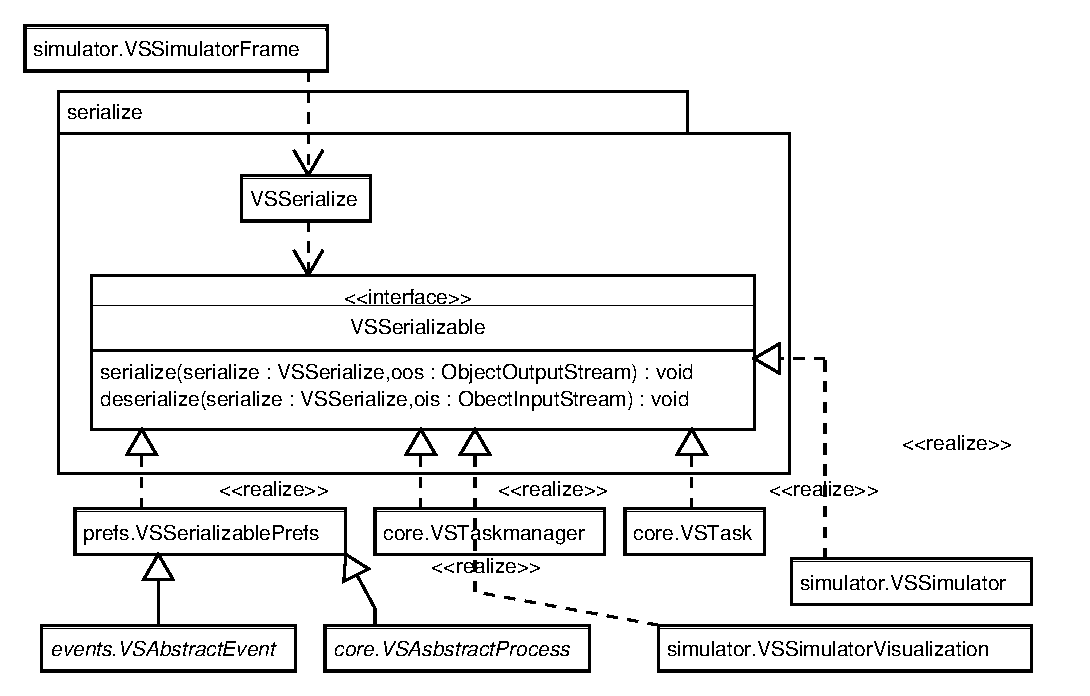
\includegraphics[width=13cm]{images/serialize}
	\caption{Das Paket \textit{serialize} und serialisierbare Klassen}
	\label{fig:PackageSerialize}
\end{figure}

Alle Klassen, die \textit{VSSerializePrefs} erweitern, k�nnen automatisch s�mtliche Einstellungen komfortabel serialisieren und deserialiseren. Beispielsweise speichert ein Simulator (\textit{VSSimulator}) alle seine globalen Simulationseinstellungen bei einer Serialisierung automatisch ab. Bei den Prozessen und den Ereignissen (und somit auch Protokollen) gilt selbiges analog. 

Abgespeicherte Simulationen sollen auch mit zuk�nftigen Versionen des Simulators kompatibel bleiben. Deshalb werden alle Objekte derjenigen Klassen, die \textit{VSSerializable} implementieren, nicht komplett serialisiert. Bei der Serialisierung werden nur relevante Klassenattribute, die der Simulationsprogrammierung- und nicht beispielsweise GUI-Komponenten angeh�ren, serialisiert. 

\subsection{Beispielimplementierung einer \textit{serialize}-Methode}

Der folgende Quelltext-Ausschnitt zeigt eine Beispielimplementierung von \textit{serialize}:

\begin{code}
    public synchronized void serialize(VSSerialize serialize,
                                       ObjectOutputStream oos)
    throws IOException {
        oss.writeObject(new Boolean(false)); // flag
        oss.writeObject(attributeOne);
        oss.writeObject(ottributeTwo);
        serialize.setObject("sampleObject", this);
        prefs.serialize(serialize, oos);
        someOtherSerializableObject.serialize(serialize, oos);
        oss.writeObject(new Boolean(false)); // flag
    }
\end{code}

Vor- und nach der eigentlichen Objektserialisierung wird jeweils ein boolesches Flag serialisiert, welches auf \textit{true} gesetzt wird, sobald in sp�teren Simulator-Versionen (was relativ unwahrscheinlich, aber m�glich ist) weitere zu serialisierende Klassenattribute hinzukommen. Eine Deserialisierung kann die Flags dann abfragen und separat behandeln. Somit bleiben �ltere bereits abgespeicherte Simulationen stets zur neusten Version des Simulators kompatibel. Wenn ein Flag auf \textit{true} gesetzt wird, dann kann unter den neuen Attributserialisierungen ein weiteres Flag gesetzt werden. Somit k�nnen beliebig viele Erweiterungen in die Serialisierung Einzug halten.

Das zu serialisierende Objekt besitzt hier lediglich zwei Attribute, die serialisiert werden sollen. Alle anderen Klassenattribute k�nnen vernachl�ssigt werden. Mit \textit{serialize.setObject} speichert \textit{serialize} eine Referenz auf das aktuelle Objekt ab, worauf andere Objektserialisierungen zur�ckgreifen k�nnen. Danach wird ein \textit{prefs} und \textit{someOtherSerializableObject} serialisiert. Die Deserialisierung folgt genau den Umgekehrten weg. Wobei hier zuerst die Instanzen der Klassen auf normalen Weg erstellt werden und dann nachtr�glich die relevanten Attribute deserialisiert und den Objekten zugewiesen werden. Hierbei werden auch mithilfe von \textit{VSSerialize} mehrere Referenzen auf das selbe Objekt korrekt behandelt.

Wenn der Anwender \textit{Datei $\rightarrow$ Simulation speichern} w�hlt, dann wird zun�chst ein \textit{VSSerialize}-Objekt erstellt. Ausgehend davon wird \textit{serialize} auf \textit{VSSimulator} ausgef�hrt (siehe Serialisierungssequenz auf Abbildung \ref{fig:SequenceSerialize}). Das Simulator-Objekt f�hrt \textit{serialize} wiederum auf das \textit{VSSimulatorVisualization}-Objekt aus. Dort wird jeder Prozess inklusive alle Protokollobjekte serialisiert. Anschlie�end folgt der Task-Manager inklusive allen programmierten Ereignissen. 


\section{Helferklassen und Klassen f�r Ausnahmebehandlungen}

\begin{figure}[h]
	\centering
	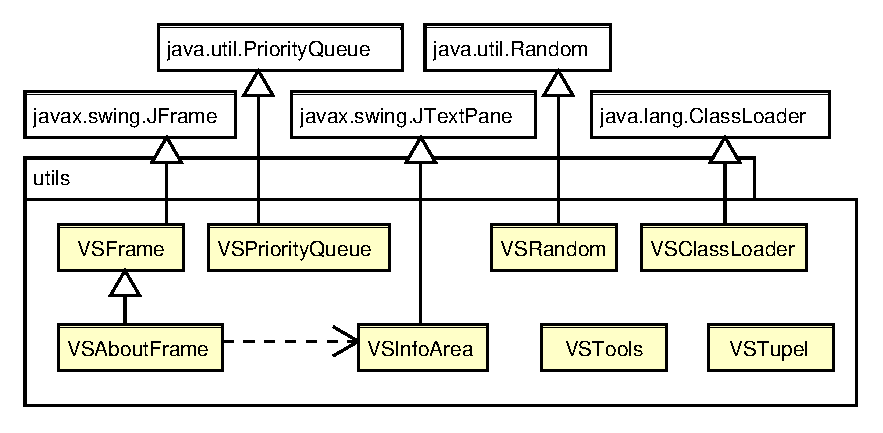
\includegraphics[width=11cm]{images/utils}
	\caption{Das Paket \textit{utils}}
	\label{fig:PackageUtils}
\end{figure}

Es wurden noch nicht die Klassen der Pakete \textit{utils} (Abbildung \ref{fig:PackageUtils}) sowie \textit{exceptions} (Abbildung \ref{fig:PackageExceptions}) vorgestellt. \textit{utils} fasst lediglich einige Helferklassen zusammen, die vom restlichen Quelltext verwendet werden.

\begin{itemize}
	\item \textit{VSFrame}: Alle Objekte, die ein eigenes Swing-Fenster besitzen, erben von der Klasse \textit{VSFrame}. Sie stellt sicher, dass neue Fenster an der richtigen Position der Bildfl�che platziert werden und dass Unterfenster (Fenster, die aus einem anderen Fenster aus ge�ffnet wurden) automatisch mit-geschlossen werden, sobald ihre ``Erzeugerfenster'' geschlossen werden. 
	\item \textit{VSAboutFrame}: Dieses Fenster implementiert die ``About-Anzeige'' die im Simulator �ber das Datei-Men� aufgerufen werden kann.
	\item \textit{VSInfoArea}: Ist f�r die Textanzeige in \textit{VSAboutFrame} zust�ndig.
	\item \textit{VSClassLoader}: Diese Klasse wird f�r die automatische Instantiierung von Ereignisobjekten ben�tigt, wenn dem Simulator lediglich die Klassennamen (aus \textit{events.VSRegisteredEvents}) bekannt sind.
	\item \textit{VSHelper}: In dieser Klasse befinden sich statische Helfermethoden, die in keine andere Klasse passen.
	\item \textit{VSPriorityQueue}: Diese Klasse wird f�r das Verwalten von \textit{core.VSTask}-Objekte im Task-Manager ben�tigt. \textit{VSPriorityQueue} passt die Priorit�ts-Warteschlange aus der Java-Standardbibliothek den Anforderungen des Simulators an.
	\item \textit{VSRandom}: Wird f�r Zufallsereignisse ben�tigt. Jedes Prozessobjekt besitzt einen solchen eigenen Pseudozufallsgenerator. Diese Klasse setzt gleichzeitig einen eigenen Seed basierend auf der lokalen Systemzeit und anderer Berechnungen fest. 
	\item \textit{VSTupel}: Diese Klasse ist eine Implementierung eines sehr einfach aufgebauten 3-Tupel Datentyps. Alle 3 Elemente k�nnen von einem anderen Typ sein, was mithilfe der Java-Generics verwirklicht wurde. \textit{VSTupel} wird von den Editorklassen f�r die Generierung von GUI-Elementen ben�tigt.
\end{itemize}

\begin{figure}[h]
	\centering
	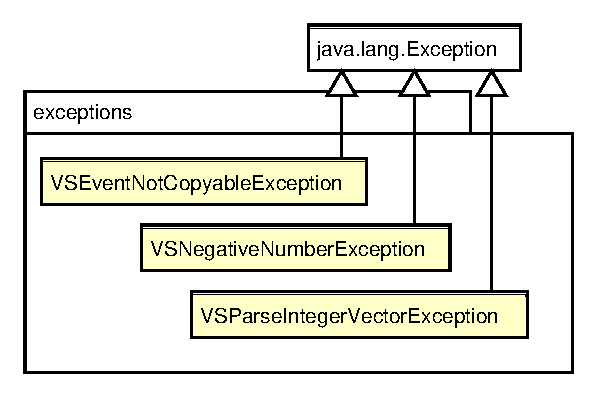
\includegraphics[width=7.5cm]{images/exceptions}
	\caption{Das Paket \textit{exceptions}}
	\label{fig:PackageExceptions}
\end{figure}

Im Paket \textit{exceptions} befinden sich lediglich einige Objekte die f�r Ausnahmebehandlungen verwendet werden. \textit{VSNotCopyableException} wird w�hrend einem Kopierversuch eines nicht-kopierbaren Ereignis geworfen. \textit{VSNegatieNumberException} wird geworfen, wenn intern negative Zahlen dort auftreten wo sie es nicht sollten. Wenn ein Editorobjekt die Benutzereingabe einer Integer-Vektor-Variable nicht parsen kann, so greifen es auf \textit{VSParseIntegerVectorException} zur�ck.

\begin{figure}
	\centering
	\rotatebox{90}{%
		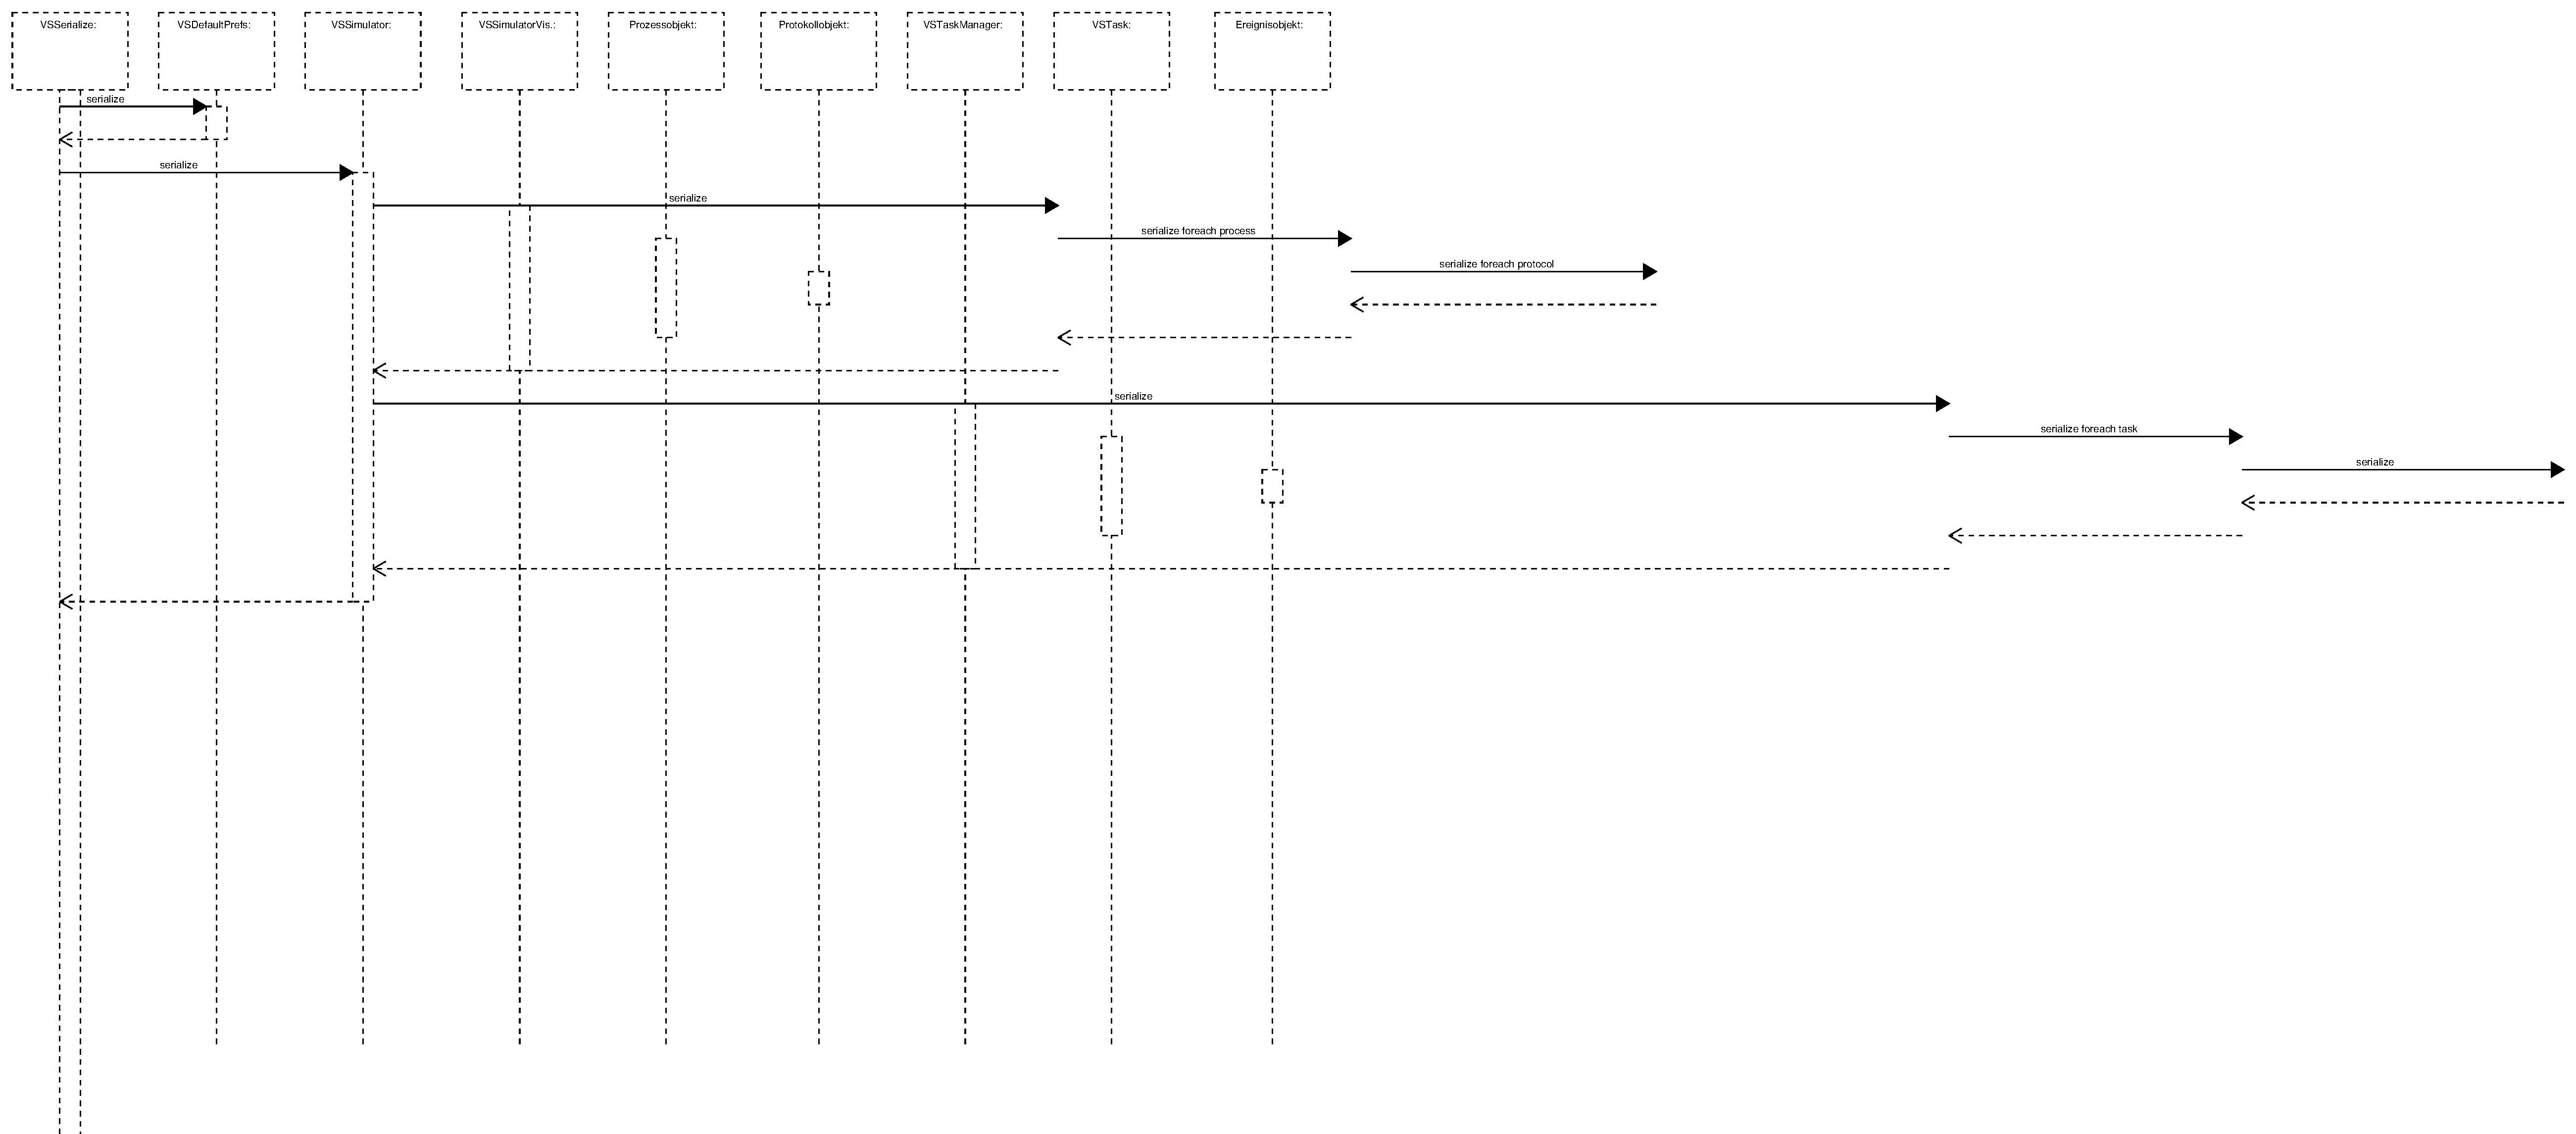
\includegraphics[width=22cm]{images/sequence-serialize}
	}
	\caption{Serialisierungssequenz}
	\label{fig:SequenceSerialize}
\end{figure}

\section{Programmierrichtlinien}

Die Programmierrichtlinien \cite{Richtlinien} entsprechen in den meisten F�llen denen aus der Vorlesung \cite{OOS}. Die Main-Methode befindet sich in der Klasse \textit{simulator.VSMain}. 

\begin{itemize}
	\item Alle Klassen- und Interfacenamen beginnen mit gro�en Buchstaben, w�hrend alle Variablen-, Methoden- und Attributnamen mit kleinen Buchstaben beginnen. Namen finaler Variablen und Attribute sind komplett in Gro�buchstaben gehalten.
	\item Alle Quelltext-Dateien besitzen einen Header, der Informationen der verwendeten Lizenz angibt.
	\item Alle Quelltext-Dateien sind vollst�ndig mit Javadoc dokumentiert worden. 
	\item Der komplette Quelltext inklusive Dokumentation werden in englischer Sprache verfasst. 
	\item Eine Quelltext-Datei hat eine maximale Zeilenl�nge von 80 Zeichen. Eine Ausnahme stellt die Klasse \textit{prefs.VSDefaultPrefs} dar, denn hier befinden sich auch l�ngere Texte die in Strings abgespeichert werden, wo manuelle Zeilenumbr�che wenig Sinn ergeben. 
	\item Es werden zuerst Klassen aus der Java-Standardbibliothek importiert, bevor Klassen aus dem VS-Simulator selbst importiert werden.
	\item F�r die Einr�ckung des Quelltextes wird das Tool \textit{astyle} mit den Aufrufparametern \textit{--style=java --mode=java} verwendet. Hierbei wird eine Einr�ckungsl�nge von 4 Zeichen verwendet.
	\item Namen abstrakter Klassen tragen stets das Prefix \textit{VSAbstract}.
	\item Namen aller Klassen und Interfaces tragen als Prefix stets \textit{VS}, was f�r Verteilte Systeme steht. 
	\item Namen aller Protokollklassen tragen als Postfix \textit{Protocol} (zum Beispiel \textit{VSPingPongProtocol}).
	\item �berall wo es Sinn ergibt werden Java-Generic-Datentypen verwendet (z.B. \textit{java.util.Vector<Integer>} anstelle von \textit{java.util.Vector}.
\end{itemize}

\section{Entwicklungsumgebung}

In diesem Teilkapitel soll ein kleiner Einblick in die Umgebung, in der der Simulator entwickelt wurde, gew�hrt werden. F�r diese Diplomarbeit wurde ausschlie�lich Open Source Software verwendet. Die einzige Ausnahme stellt Microsoft Windows XP dar, worauf der Simulator zus�tzlich getestet wurde. Der Simulator wurde jedoch haupts�chlich unter dem Betriebssystem FreeBSD 7.0, was ein open source Unix-Derivat ist, programmiert. 

Wie bereits bekannt ist, wurde Sun's Java, was mittlerweile auch Open Source Software ist, in der Version 6 (1.6) als die Implementierungssprache gew�hlt und f�r die Quelltextdokumentation kam Javadoc- und f�r die automatische Quelltexteinr�ckung astyle zum Einsatz. Als Built-Tool wurde hier auf Apache Ant gesetzt. F�r die Erstellung dieses PDF-Dokumentes wurde LaTeX in Verbindung mit dem Built-Tool GNU Make und Rubber verwendet. Eine Rechtschreib�berpr�fung wurde mit aspell sowie OpenOffice.org durchgef�hrt. xPDF diente als PDF-Anzeigeprogramm.

Als Versionierungssystem wurde SVN (Subversion) verwendet. F�r den Zugriff auf das SVN-Repository mittels HTTPS (Hypertext Transfer Protocol Secure) wurde der Apache-Webserver mit WebDAV-Plugin verwendet. Zudem kam WebSVN als Webschnittstelle des SVN-Repository zum Einsatz. Mozilla Firefox diente f�r das Betrachten der Javadocs und der WebSVN-Oberfl�che.

F�r schreiben von Java-Quelltext wurde GVim (Graphical Vi IMproved) sowie Eclipse verwendet. Eclipse unterst�tzt bessere Code-Refactoring-Methoden, w�hrend GVim mit seiner Flexibilit�t und schnelleren Editierm�glichkeiten und mit Vim-Script, der eigenen Script-Engine, gl�nzt. Es wurden au�erdem das JAutoDoc- (f�r die Erstellung von Javadoc-Kommentare) und das Subversion-Eclipse-Plugin verwendet. Je nach Zweck wurde zwischen diesen beiden Umgebungen gewechselt. F�r das Verfassen des LaTeX-Dokumentes wurde GVim verwendet.

S�mtliche UML-Diagramme wurden mit ArgoUML angefertigt und die Screenshots mit The GIMP (GNU Image Manipulation Program) sowie ImageMagick nachbearbeitet. Mit dem zip-Programm wurden alle VS-Simulator Distributionen verpackt.

\subsubsection{Linkliste der verwendeten Software}

\begin{itemize}
	\setlength{\itemsep}{-2mm}
	\item Apache Webserver - \url{http://httpd.apache.org}	
	\item ArgoUML - \url{http://argouml.tigris.org}
	\item Eclipse - \url{http://www.eclipse.org}
	\item FreeBSD - \url{http://www.FreeBSD.org}
	\item GNU Make - \url{http://www.gnu.org/software/make}
	\item GVim - \url{http://www.vim.org}
	\item ImageMagick - \url{http://www.imagemagick.org}
	\item Javadoc - \url{http://java.sun.com/j2s2/javadoc}
	\item Mozilla Firefox - \url{http://www.mozilla.com}
	\item OpenOffice.org - \url{http://www.OpenOffice.org}
	\item Rubber - \url{http://www.pps.jussieu.fr/~beffara/soft/rubber}
	\item Sun Java - \url{http://java.sun.com}
	\item The GIMP - \url{http://www.gimp.org}
	\item WebDAV - \url{http://httpd.apache.org/docs/2.0/mod/mod\_dav.html}	
	\item WebSVN - \url{http://websvn.tigris.org}
	\item aspell - \url{http://aspell.sourceforge.net}
	\item astyle - \url{http://astyle.sourceforge.net}
	\item xPDF - \url{http://www.foolabs.com/xpdf}
	\item zip - \url{http://www.info-zip.org/Zip.html}
\end{itemize}


\input{chapters/ausblick}

\appendix

\input{chapters/anhang-a}

\bibliographystyle{alpha}
\bibliography{bib/referenzen}
%\printindex
\end{document}

%
% EOF
%

